\chapter{Implementation}\label{cha:implementation}

This chapters describes the implementation done in PyTorch for this thesis. The first part details the methods evaluated in depth and ego motion prediction, the second part describes the implementation of unsupervised keypoint prediction, and the last part describes how the consensus maximization network was implemented.



\subsection{Architectures for depth and ego motion CNNs}

In order to predict depth and motion from monocular images two different CNN architectures are examined. Both are encoder-decoder type architectures, and their general layout is illustrated in Figure \ref{fig:net}.

The first architecture is referred to as SfMlearner\cite{sfmlearner}, and uses a DispNet\cite{dispnet} architecture is used to predict depth maps at four different scales.

The second architecture is referred to as Monodepth2\cite{monodepth2}, and uses a ResNet18 architecture instead of a DispNet architecture to predict depth estimates. This architecture is a smaller resulting in faster training and evaluation.

Both SfMlearner and Monodepth2 uses a separate network to predict poses between frames. The pose network has a ResNet18\cite{resnet} architecture, but the decoder is modified to predict pose updates in an euler angle axis representation.

\begin{figure}[H]
	\centering
	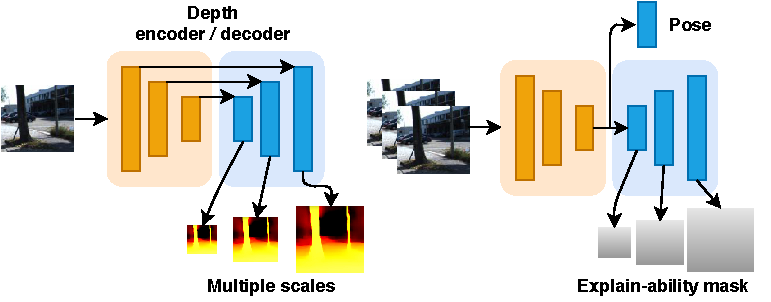
\includegraphics[width=1.0\textwidth]{net}
	\caption{High level diagram of the network architectures used for depth and ego motion prediction. The layers from the depth encoder are concatenated into the layers of the decoder. Depth maps are computed at multiple scales in the decoder and are all used in the loss function. A separate network that takes as input 3 subsequent frames predicts the poses $\textbf{T}_{t\rightarrow t-1}$ and $\textbf{T}_{t\rightarrow t+1}$ between the target and nearby reference frames. The pose network shares encoder with the explain-ability mask predicting network (section \ref{sec:modellimit}).}
	\label{fig:net}
\end{figure}

\subsection{Differentiable depth image warping}
\label{sec:diffwarp}

The core component of unsupervised depth learning is the differentiable depth image warp operation in the loss function of the CNN networks. Given the intrinsic camera matrix:

\begin{equation}
\textbf{K} = 
\begin{pmatrix}
f_\mathrm{x} & s & x_0 \\
0 & f_\mathrm{y} & y_0 \\
0 & 0   & 1
\end{pmatrix}
\end{equation}

And the predicted depth $ D_t(p_t) $ of pixel $ p_t $ of the target (current) frame. And the transform $ T_{t \rightarrow s} $ from the target to source (next/previous) frame:

\begin{equation}
\textbf{T}_{t \rightarrow s} =
\begin{pmatrix}
\textbf{R} & \textbf{t} \\
0 & 1
\end{pmatrix}
\end{equation}

The position of the target pixel $ p_t $ in the source image $ p_s $ can be calculated in homogeneous coordinates as:

\begin{equation}
\textbf{p}_s \sim 
\begin{pmatrix}
\textbf{K}  & \textbf{0} \\
\end{pmatrix}
\textbf{T}_{t \rightarrow s} \textbf{D}_t(\textbf{p}_t) \textbf{K}^{-1} \textbf{p}_t 
\end{equation}

The pixel position $ p_s $ is however continuous and in order to sample the discrete source image $ \textbf{I}_s $ a differentiable bilinear sampling method is used. The method is described in \textit{spatial transformer networks}\cite{spatialtransformernetworks} and works by interpolating the neighbouring 4 pixels values (top-left, bottom-right) by the distance to the the continuous sampling point $ p_t $. This process is illustrated in Figure \ref{fig:warp}.


\begin{figure}[H]
	\centering
	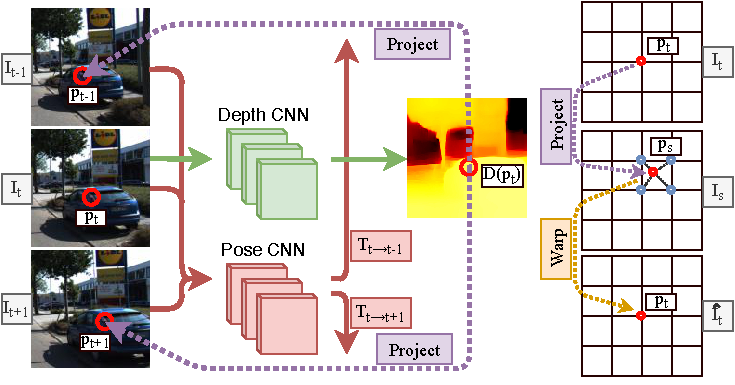
\includegraphics[width=1.0\textwidth]{warp}
	\caption{The \abbrCNN predicts the depth map $\textbf{D}$ of the target image $\textbf{I}_t$, and also the relative movement, $\textbf{T}_{t\rightarrow t-1}, \textbf{T}_{t\rightarrow t+1}$ between the target image and the source images. Each pixel $p_t$ in the target image is projected onto a position in the source images which are sampled using bilinear interpolation. This should recreate the appearance of the target image but with pixels sampled from the source image. An appearance similarity metric between the original target image and the recreated target images can be used as the loss function for the \abbrCNN to learn to accurately predict correct depth and movement.}
	\label{fig:warp}
\end{figure}

%TODO: Insert examples of warped/recreated and diff images between target and recreated images.....


\subsection{Loss functions}
\label{sec:loss}

In order to learn the objective of depth and ego motion prediction, different combinations of the following loss terms where evaluated.

To measure the similarity of the target image $\textbf{I}_t$ and the reconstructed image $\hat{\textbf{I}}_t$ a photometric loss term defined as the mean of the absolute value of the difference of pixel intensities of the two images was used.

\begin{equation}
\mathcal{L}_p(\textbf{I}_t, \hat{\textbf{I}}_t)=\mean(|\textbf{I}_t - \hat{\textbf{I}}_t|)
\end{equation}

Another photometric loss term evaluated in this thesis is based on structured similarity, referred to as SSIM\cite{ssim}. It was originally developed to measure the quality of digital television, comparing a compressed digital image to the original distortion-free image.

\begin{equation}
\mathcal{L}_{ssim}(\textbf{I}_t, \hat{\textbf{I}}_t)=\mean(\clamp(\textbf{0},\textbf{1},\dfrac{\textbf{1}-\SSIM(\textbf{I}_t, \hat{\textbf{I}}_t)}{2}))
\end{equation}
\begin{equation}
\SSIM(x,y)=\frac{(2\mu_x\mu_y+C_1)(2\sigma_{xy}+C_2)}{(\mu_x^2+\mu_y^2+C_1)(\sigma_x^2+\sigma_y^2+C_2)}
\end{equation}

with $C_1=1e-4$ and $C_2=9e-4$. To compute the per-patch mean $\mu_x$ and standard deviation $\sigma_x$, a 1 pixel reflection padding was first used on the edges of the input images and then a $3\times3$ average pool filter with stride 1 was used to get the mean. Then $ \sigma_x=\mu_{x^2}-\mu_x^2 $.

The two above mentioned photometric loss terms can also be combined and balanced using $ \mathcal{L}_{ps}(\textbf{I}_t, \hat{\textbf{I}}_s) = \alpha \mathcal{L}_{ssim} + (1-\alpha) \mathcal{L}_p $. In the experiments of this thesis $\alpha=0.85$ was used, which is the same value used in the original Monodepth2 paper. As the network learns over time to predict more accurate depth and ego motion, the reconstruction loss will decrease. The loss per individual pixel is illustrated in Figure \ref{fig:diff}, which shows the loss from the same sample but after 1 and 30 epochs of training respectively.

\begin{figure}[H]
	\centering
	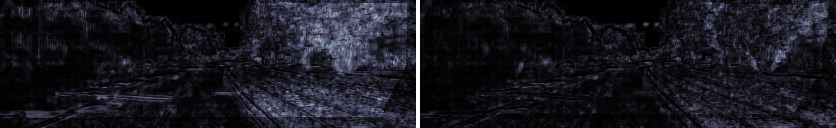
\includegraphics[width=1.0\textwidth]{diff}
	\caption{The images illustrates the photometric reconstruction loss $ \mathcal{L}_{ps} $ for each pixel in a reconstructed image for the same frame but after different length of training. The left image shows the loss after 1 epoch of training and the right image shows the loss after 30 epochs. The reconstruction loss should decrease during training as the network learns to predict better depth maps, which is what we see.}
	\label{fig:diff}
\end{figure}

To propagate the depth from textured regions to regions of uniform color a depth smoothness loss term is used. The first alternative is a loss on the second derivative of the depth intensities. This loss term will discourage the network to predict fluctuating depth values in regions of uniform color such as the pavement, that should be smooth. The drawback of this technique is that changes in depth values are penalized equally in regions where there are a lot of detail that therefore could be lost in the depth map.

\begin{equation}
\mathcal{L}_{smooth}(\textbf{D}_t)=\mean(|\delta_x^2 \textbf{D}_t|+|\delta_y^2 \textbf{D}_t|)
\end{equation}

The second alternative investigated was an edge aware smoothness loss that weights the first order derivative of the depth map with the exponential of the first derivative of the pixel intensities. This method allows large changes in depth near sharp features in the image but penelizes changes in depth in smooth regions, see Figure \ref{fig:edge}. The method showed great promise, resulting in sharper edges because the smoothness term is weighted to mostly affect areas with small photometric derivative.

\begin{equation}
\mathcal{L}_{edge}(\textbf{D}_t)=\mean(|\delta_x \textbf{D}_t|e^{-|\delta_x \textbf{I}_t|} + |\delta_y \textbf{D}_t|e^{-|\delta_y \textbf{I}_t|})
\end{equation}

\begin{figure}[H]
	\centering
	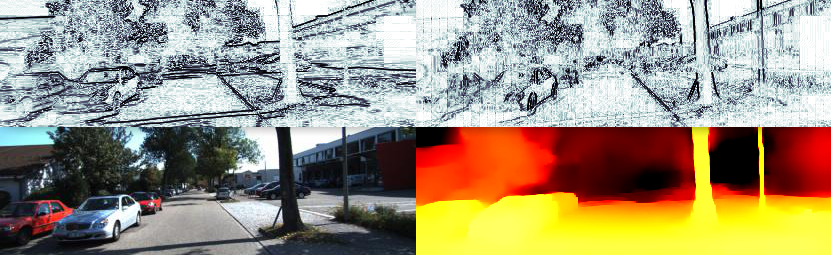
\includegraphics[width=0.9\textwidth]{edge}
	\caption{The top row of images illustrates the edge weighting terms $e^{-|\delta_y \textbf{I}_t|}$ and $e^{-|\delta_x \textbf{I}_t|}$ respectively. The weight is near 0 at the edges of tree trunks and near 1 on the pavement. This will preserve the details in the depth map around trees but keep the pavement smooth.}
	\label{fig:edge}
\end{figure}

\subsection{Depth map normalization}\label{sec:normalization}

The predicted depth is scale invariant which can make it difficult to balance the loss terms with the correct weights. To alleviate this is issue the depth map can be normalized before it is used in the loss.

\begin{equation}
\hat{\textbf{D}_t} = \frac{\textbf{D}_t}{\median(\textbf{D}_t)} 
\end{equation}

\subsection{Depth map up-scaling}\label{sec:upscale}

The smaller depth maps in the depth decoder of the network are all used in the loss. Early work in this area down-scaled the target image to fit the size of the smaller depth maps when used in the loss function. But in MonoDepth2\cite{monodepth2} it was proposed to instead up-scale the depth maps to the original target image size, see Figure \ref{fig:upscale}.

\begin{figure}[H]
	\centering
	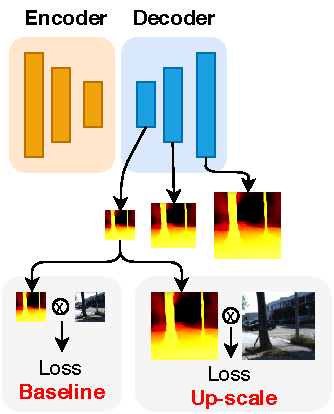
\includegraphics[width=0.3\textwidth]{upscale}
	\caption{The depth maps can optionally be up-scaled in the loss function.}
	\label{fig:upscale}
\end{figure}

\subsection{Handling occlusions}
\label{sec:occlusion}

\iffalse
\paragraph{Disparity loss} To encourage background depths (low disparities) in shadows of the depth map where occlusion has occurred a penalty on the disparity can be added $ \mathcal{L}_{o} =|d_t|. $
\fi

In the SfMLearner paper the photometric loss is calculated for the previous and next frames compared to the current in the sequence. The pixel wise average across the frames are then used. This causes problems if a pixel is for example occluded in the previous frame, but visible in the current and next frame. In this situation the average loss will be large even though a correct depth and transformation has been predicted, because of the occluded pixel. Instead Monodepth2 suggests to pick the minimum per pixel error over the frames which alleviates this issue, see Figure \ref{fig:min}. Both techniques where implemented in this thesis and compared in the experiments.

\begin{figure}[H]
	\centering
	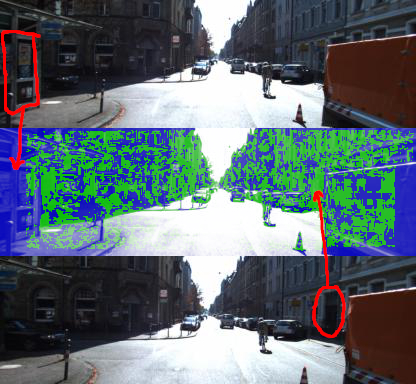
\includegraphics[width=0.5\textwidth]{min}
	\caption{By picking the per pixel minimum reprojection error the issue created by occluded pixels can be alleviated. The top image is the previous frame, the middle image is the current target frame and the bottom image is the next frame in the sequence. If the minimum reprojection error can be found in the previous frame then it is colored blue, if its from the next frame it is green. Because the door to the right is occluded by the orange truck in the previous frame, the reprojection loss from the next frame is used instead where the door is visible. The wall to the left is outside the boundaries of the next image, so the reprojection error from the previous frame is used instead.}
	\label{fig:min}
\end{figure}

\subsection{Handling model limitations}
\label{sec:modellimit}

In order to optimize using the photometric reprojecton error as the loss function two assumptions must hold. Firstly the scene must be static, meaning all objects in the scene must be still except the moving camera. Dynamic objects will cause problems. Secondly there must be photometric consistency between frames for the photometric error to make sense. This means that non lambertian surfaces, change in lighting, and change in exposure between frames will cause problems. Two different methods of dealing with this issue was implemented and evaluated in this thesis.

\paragraph{Explainability mask} The authors of \cite{sfmlearner} tackle this problem by having a CNN predict what pixels are valid to use in the photometric loss function, see Figure~\ref{fig:exp}. It shares the encoder of the pose predicting network but branches of into a different decoders which estimates a mask of the valid/explainable pixels. The loss function for the mask is the cross entropy loss compared to a mask filled with ones. The photometric loss function is augmented to include the explainability mask removing pixels that cannot be explained by the predicted depth and transformation. This encourages the mask to be filled with ones, but allows some slack due to pixels that can not be explained by the photometric loss.

\begin{figure}[H]
	\centering
	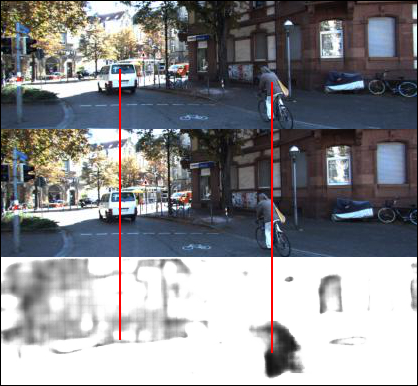
\includegraphics[width=0.5\textwidth]{exp}
	\caption{This is an image extracted from the experiments in this thesis. The top image is frame $\textbf{I}_t$ the middle image is frame $\textbf{I}_{t-1}$ and the last image is the explain-ability mask. It is visible that the network correctly predicts that the bicycle is not moving in relation to the camera, but it does not remove pixels from the white van as it should.}
	\label{fig:exp}
\end{figure}

\paragraph{Stationary pixels mask} The authors of \cite{monodepth2} introduced a mask to remove stationary pixels from the set of previous, current and next frame. This is done by creating a mask where the photometric error is smaller before applying the projection than after. This works because pixels from objects that have not moved in relation to the camera will of course have a small photometric loss without reprojection. This will remove pixels from the car dashboard and also nearby vehicles that are traveling at the same speed, see Figure \ref{fig:stat}.

\begin{figure}[H]
	\centering
	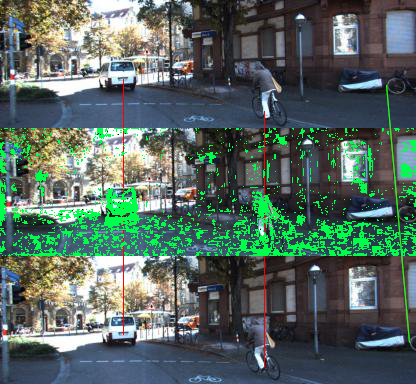
\includegraphics[width=0.5\textwidth]{stat}
	\caption{The black pixels in the image are the ones removed because their photometric error is smaller before warping the image using the depth map compared to after warping. The red horizontal lines on the van and bicyclist illustrates that they do not move with respect to the camera, and the green slanted line illustrates that the bike leaning on the wall is moving with respect to the camera. The mask successfully removes pixels on the van and bicyclist, but also removes some pixels on the pavement that should not be removed.}
	\label{fig:stat}
\end{figure}

\newpage
\section{Unsupervised keypoint learning}

In order to build a map it is useful to extract features, or keypoints, from images. Every keypoints should have a unique descriptor which can be used to identify it in the map which makes it possible to expand the map and also localize the camera. How to build a map and localize in it is out of scope for this thesis. This section will describe the usnupervised learning method implemented in this thesis, to extract keypoints from images.

The method evaluated in this thesis is based on the UnsuperPoint paper\cite{unsuperpoint}. The network architecture is illustrated in Figure \ref{fig:unsuperpoint}. The input image is fed into a shared backbone. The features from the backbone are then split into three different encoders that estimate the score, position and a descriptor for each keypoint. The network will estimate a keypoint in every $8\times 8$ patch of the image, but only the top $N$ keypoints sorted by score are used in the evaluation.

\begin{figure}[H]
	\centering
	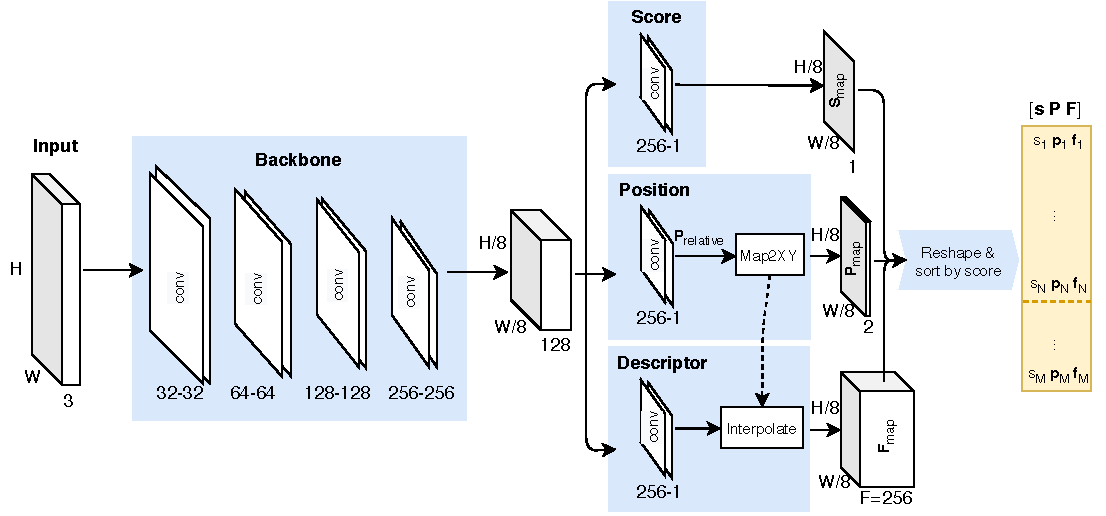
\includegraphics[width=1.0\textwidth]{unsuperpoint}
	\caption{The network has a common backbone and then splits into separate score, position and descriptor encoders. The output is reshaped and sorted by descending score.}
	\label{fig:unsuperpoint}
\end{figure}

The score encoder is terminated by a sigmoid function and outputs $S_{map}$, containing scores between 0 and 1 for each keypoint. The purpose of the scores are to rank the quality of the keypoints in all $8\times 8$px patches of the image and only pick the best ones. Typically patches in the sky and other non-textured areas will have keypoints with low scores.

The position encoder is also terminated by a sigmoid function and outputs $P_{relative}$ which is the relative position of the keypoint in each patch. In the Map2XY block in Figure \ref{fig:unsuperpoint} the relative positions are converted to absolute pixel positions to form $P_{map}$.

\[
P_{map,x}(r,c) = 8 * (c + P_{relative,x}(r,c))
\]
\[
P_{map,y}(r,c) = 8 * (r + P_{relative,y}(r,c))
\]

The descriptor encoder predicts a descriptor vector of length $256$ for each keypoint. The purpose of the descriptor is to find corresponding keypoints in different images. The encoder produces 1 descriptor vector for each $8\times 8$ patch in the image. This vector can be used directly as the keypoint descriptor and it works pretty well. Even better results can be achieved using the absolute keypoint positions to sample the values in the descriptor map with the same interpolation method used to do the warping in Figure \ref{fig:warp}.

$S_{map}$, $P_{map}$ and $F_{map}$ are reshaped into a vector $s$ of $M$ elements, an $M\times 2$ matrix $P$ and an $M\times 255$ matrix $F$, where $M=\frac{W}{8}*\frac{H}{8}=832$.

The network is trained in a siamese twin setup, where two duplicate networks that share weights are fed different inputs and the loss is formulated by comparing the output scores, positions and descriptors.

\begin{figure}[H]
	\centering
	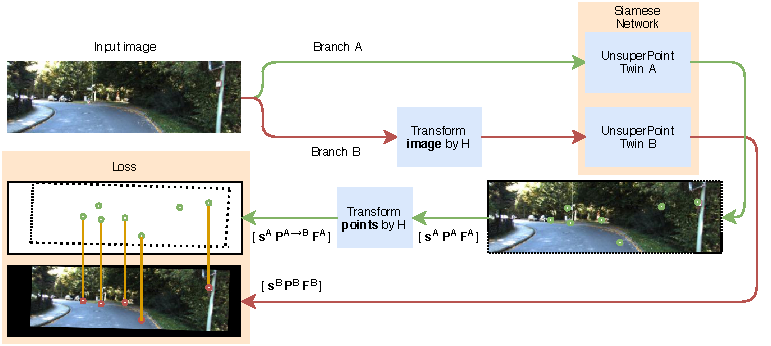
\includegraphics[width=1.0\textwidth]{unsuperpointloss}
	\caption{This figure illustrates the flow from input image to loss function. The image from branch A is fed directly into the UnsuperPoint network, while in branch B the image is first transformed by a random homography $H$. The keypoint positions from twin A are transformed by the same homography $H$ and the output from the two branches are compared in order to formulate the loss function.}
	\label{fig:unsuperpointloss}
\end{figure}

For each branch $b\in\{A,B\}$ the siamese networks output the reshaped matrices $s^b$, $P^b$ and $F^b$ which contain the scores, positions and descriptors of the $M$ points in each image.

\subsection{Loss function for keypoint learning}\label{sec:keypointloss}

To formulate the loss function the point correspondences between branch A and B need to be determined. The points in branch A are transformed such that $p_i^{A\rightarrow B}=Hp_i^A$. Then an $M^A\times M^B$ distance matrix $G$ is calculated from the pairwise distances between all points in each branch.

\[
G=[g_{ij}]_{M^A\times M^B}=\left[||p_i^{A\rightarrow B}-p_j^B||\right]_{M^A\times M^B}
\]

We define a point pair if point $i$ in branch A has a point $j$ as its closest neightbor in branch B, and if the distance $g_{ij}$ is less than 8px. With the point pairs defined the output matrices $s^b$, $P^b$ and $F^b$ can be redefined as \textit{corresponding matrices} $\hat{s}^b$, $\hat{P}^b$ and $\hat{F}^b$ with $K\le M$ entries, such that entry $k$ in the new matrices maps to corresponding points in the input images.

Define $d_k$ as the distance between each point pair.

\[
d_k=||\hat{p}_k^{A\rightarrow B}-\hat{p}_k^B||
\]

The distance between point pairs should be minimized, this is achieved by the $\mathcal{L}^{position}$ loss term.

\[
\mathcal{L}_k^{position} = d_k
\]

The scores of point pairs in branch A and B should be similar, this is achieved by the $\mathcal{L}^{sim}$ loss term.

\[
\mathcal{L}_k^{sim} = \left(\hat{s}_k^{A}-\hat{s}_k^B\right)^2
\]

To teach the network to predict sensible scores for the points, the distance $d_k$ between point pairs is used.

\[
\mathcal{L}_k^{score}=\frac{\hat{s}_k^A+\hat{s}_k^B}{2}\left(d_k-\bar{d}\right)
\]

If $d_k$ is less than the mean distance $\bar{d}$ the score should be large in order to minimize the loss. If the $d_k$ is greater than the mean distance $\bar{d}$ the score should be small in order to minimize the loss.

\begin{figure}[H]
	\begin{center}
		%% Creator: Matplotlib, PGF backend
%%
%% To include the figure in your LaTeX document, write
%%   \input{<filename>.pgf}
%%
%% Make sure the required packages are loaded in your preamble
%%   \usepackage{pgf}
%%
%% Figures using additional raster images can only be included by \input if
%% they are in the same directory as the main LaTeX file. For loading figures
%% from other directories you can use the `import` package
%%   \usepackage{import}
%% and then include the figures with
%%   \import{<path to file>}{<filename>.pgf}
%%
%% Matplotlib used the following preamble
%%
\begingroup%
\makeatletter%
\begin{pgfpicture}%
\pgfpathrectangle{\pgfpointorigin}{\pgfqpoint{2.864820in}{2.100000in}}%
\pgfusepath{use as bounding box, clip}%
\begin{pgfscope}%
\pgfsetbuttcap%
\pgfsetmiterjoin%
\definecolor{currentfill}{rgb}{1.000000,1.000000,1.000000}%
\pgfsetfillcolor{currentfill}%
\pgfsetlinewidth{0.000000pt}%
\definecolor{currentstroke}{rgb}{1.000000,1.000000,1.000000}%
\pgfsetstrokecolor{currentstroke}%
\pgfsetdash{}{0pt}%
\pgfpathmoveto{\pgfqpoint{0.000000in}{0.000000in}}%
\pgfpathlineto{\pgfqpoint{2.864820in}{0.000000in}}%
\pgfpathlineto{\pgfqpoint{2.864820in}{2.100000in}}%
\pgfpathlineto{\pgfqpoint{0.000000in}{2.100000in}}%
\pgfpathclose%
\pgfusepath{fill}%
\end{pgfscope}%
\begin{pgfscope}%
\pgfsetbuttcap%
\pgfsetmiterjoin%
\definecolor{currentfill}{rgb}{1.000000,1.000000,1.000000}%
\pgfsetfillcolor{currentfill}%
\pgfsetlinewidth{0.000000pt}%
\definecolor{currentstroke}{rgb}{0.000000,0.000000,0.000000}%
\pgfsetstrokecolor{currentstroke}%
\pgfsetstrokeopacity{0.000000}%
\pgfsetdash{}{0pt}%
\pgfpathmoveto{\pgfqpoint{0.358102in}{0.231000in}}%
\pgfpathlineto{\pgfqpoint{2.578338in}{0.231000in}}%
\pgfpathlineto{\pgfqpoint{2.578338in}{1.848000in}}%
\pgfpathlineto{\pgfqpoint{0.358102in}{1.848000in}}%
\pgfpathclose%
\pgfusepath{fill}%
\end{pgfscope}%
\begin{pgfscope}%
\pgfpathrectangle{\pgfqpoint{0.358102in}{0.231000in}}{\pgfqpoint{2.220236in}{1.617000in}}%
\pgfusepath{clip}%
\pgfsetbuttcap%
\pgfsetmiterjoin%
\definecolor{currentfill}{rgb}{0.000000,0.000000,1.000000}%
\pgfsetfillcolor{currentfill}%
\pgfsetlinewidth{0.000000pt}%
\definecolor{currentstroke}{rgb}{0.000000,0.000000,0.000000}%
\pgfsetstrokecolor{currentstroke}%
\pgfsetstrokeopacity{0.000000}%
\pgfsetdash{}{0pt}%
\pgfpathmoveto{\pgfqpoint{0.459022in}{0.231000in}}%
\pgfpathlineto{\pgfqpoint{0.499390in}{0.231000in}}%
\pgfpathlineto{\pgfqpoint{0.499390in}{0.956146in}}%
\pgfpathlineto{\pgfqpoint{0.459022in}{0.956146in}}%
\pgfpathclose%
\pgfusepath{fill}%
\end{pgfscope}%
\begin{pgfscope}%
\pgfpathrectangle{\pgfqpoint{0.358102in}{0.231000in}}{\pgfqpoint{2.220236in}{1.617000in}}%
\pgfusepath{clip}%
\pgfsetbuttcap%
\pgfsetmiterjoin%
\definecolor{currentfill}{rgb}{0.000000,0.000000,1.000000}%
\pgfsetfillcolor{currentfill}%
\pgfsetlinewidth{0.000000pt}%
\definecolor{currentstroke}{rgb}{0.000000,0.000000,0.000000}%
\pgfsetstrokecolor{currentstroke}%
\pgfsetstrokeopacity{0.000000}%
\pgfsetdash{}{0pt}%
\pgfpathmoveto{\pgfqpoint{0.499390in}{0.231000in}}%
\pgfpathlineto{\pgfqpoint{0.539758in}{0.231000in}}%
\pgfpathlineto{\pgfqpoint{0.539758in}{0.515078in}}%
\pgfpathlineto{\pgfqpoint{0.499390in}{0.515078in}}%
\pgfpathclose%
\pgfusepath{fill}%
\end{pgfscope}%
\begin{pgfscope}%
\pgfpathrectangle{\pgfqpoint{0.358102in}{0.231000in}}{\pgfqpoint{2.220236in}{1.617000in}}%
\pgfusepath{clip}%
\pgfsetbuttcap%
\pgfsetmiterjoin%
\definecolor{currentfill}{rgb}{0.000000,0.000000,1.000000}%
\pgfsetfillcolor{currentfill}%
\pgfsetlinewidth{0.000000pt}%
\definecolor{currentstroke}{rgb}{0.000000,0.000000,0.000000}%
\pgfsetstrokecolor{currentstroke}%
\pgfsetstrokeopacity{0.000000}%
\pgfsetdash{}{0pt}%
\pgfpathmoveto{\pgfqpoint{0.539758in}{0.231000in}}%
\pgfpathlineto{\pgfqpoint{0.580126in}{0.231000in}}%
\pgfpathlineto{\pgfqpoint{0.580126in}{0.395466in}}%
\pgfpathlineto{\pgfqpoint{0.539758in}{0.395466in}}%
\pgfpathclose%
\pgfusepath{fill}%
\end{pgfscope}%
\begin{pgfscope}%
\pgfpathrectangle{\pgfqpoint{0.358102in}{0.231000in}}{\pgfqpoint{2.220236in}{1.617000in}}%
\pgfusepath{clip}%
\pgfsetbuttcap%
\pgfsetmiterjoin%
\definecolor{currentfill}{rgb}{0.000000,0.000000,1.000000}%
\pgfsetfillcolor{currentfill}%
\pgfsetlinewidth{0.000000pt}%
\definecolor{currentstroke}{rgb}{0.000000,0.000000,0.000000}%
\pgfsetstrokecolor{currentstroke}%
\pgfsetstrokeopacity{0.000000}%
\pgfsetdash{}{0pt}%
\pgfpathmoveto{\pgfqpoint{0.580126in}{0.231000in}}%
\pgfpathlineto{\pgfqpoint{0.620494in}{0.231000in}}%
\pgfpathlineto{\pgfqpoint{0.620494in}{0.380515in}}%
\pgfpathlineto{\pgfqpoint{0.580126in}{0.380515in}}%
\pgfpathclose%
\pgfusepath{fill}%
\end{pgfscope}%
\begin{pgfscope}%
\pgfpathrectangle{\pgfqpoint{0.358102in}{0.231000in}}{\pgfqpoint{2.220236in}{1.617000in}}%
\pgfusepath{clip}%
\pgfsetbuttcap%
\pgfsetmiterjoin%
\definecolor{currentfill}{rgb}{0.000000,0.000000,1.000000}%
\pgfsetfillcolor{currentfill}%
\pgfsetlinewidth{0.000000pt}%
\definecolor{currentstroke}{rgb}{0.000000,0.000000,0.000000}%
\pgfsetstrokecolor{currentstroke}%
\pgfsetstrokeopacity{0.000000}%
\pgfsetdash{}{0pt}%
\pgfpathmoveto{\pgfqpoint{0.620494in}{0.231000in}}%
\pgfpathlineto{\pgfqpoint{0.660862in}{0.231000in}}%
\pgfpathlineto{\pgfqpoint{0.660862in}{0.350612in}}%
\pgfpathlineto{\pgfqpoint{0.620494in}{0.350612in}}%
\pgfpathclose%
\pgfusepath{fill}%
\end{pgfscope}%
\begin{pgfscope}%
\pgfpathrectangle{\pgfqpoint{0.358102in}{0.231000in}}{\pgfqpoint{2.220236in}{1.617000in}}%
\pgfusepath{clip}%
\pgfsetbuttcap%
\pgfsetmiterjoin%
\definecolor{currentfill}{rgb}{0.000000,0.000000,1.000000}%
\pgfsetfillcolor{currentfill}%
\pgfsetlinewidth{0.000000pt}%
\definecolor{currentstroke}{rgb}{0.000000,0.000000,0.000000}%
\pgfsetstrokecolor{currentstroke}%
\pgfsetstrokeopacity{0.000000}%
\pgfsetdash{}{0pt}%
\pgfpathmoveto{\pgfqpoint{0.660862in}{0.231000in}}%
\pgfpathlineto{\pgfqpoint{0.701230in}{0.231000in}}%
\pgfpathlineto{\pgfqpoint{0.701230in}{0.350612in}}%
\pgfpathlineto{\pgfqpoint{0.660862in}{0.350612in}}%
\pgfpathclose%
\pgfusepath{fill}%
\end{pgfscope}%
\begin{pgfscope}%
\pgfpathrectangle{\pgfqpoint{0.358102in}{0.231000in}}{\pgfqpoint{2.220236in}{1.617000in}}%
\pgfusepath{clip}%
\pgfsetbuttcap%
\pgfsetmiterjoin%
\definecolor{currentfill}{rgb}{0.000000,0.000000,1.000000}%
\pgfsetfillcolor{currentfill}%
\pgfsetlinewidth{0.000000pt}%
\definecolor{currentstroke}{rgb}{0.000000,0.000000,0.000000}%
\pgfsetstrokecolor{currentstroke}%
\pgfsetstrokeopacity{0.000000}%
\pgfsetdash{}{0pt}%
\pgfpathmoveto{\pgfqpoint{0.701230in}{0.231000in}}%
\pgfpathlineto{\pgfqpoint{0.741598in}{0.231000in}}%
\pgfpathlineto{\pgfqpoint{0.741598in}{0.313233in}}%
\pgfpathlineto{\pgfqpoint{0.701230in}{0.313233in}}%
\pgfpathclose%
\pgfusepath{fill}%
\end{pgfscope}%
\begin{pgfscope}%
\pgfpathrectangle{\pgfqpoint{0.358102in}{0.231000in}}{\pgfqpoint{2.220236in}{1.617000in}}%
\pgfusepath{clip}%
\pgfsetbuttcap%
\pgfsetmiterjoin%
\definecolor{currentfill}{rgb}{0.000000,0.000000,1.000000}%
\pgfsetfillcolor{currentfill}%
\pgfsetlinewidth{0.000000pt}%
\definecolor{currentstroke}{rgb}{0.000000,0.000000,0.000000}%
\pgfsetstrokecolor{currentstroke}%
\pgfsetstrokeopacity{0.000000}%
\pgfsetdash{}{0pt}%
\pgfpathmoveto{\pgfqpoint{0.741598in}{0.231000in}}%
\pgfpathlineto{\pgfqpoint{0.781966in}{0.231000in}}%
\pgfpathlineto{\pgfqpoint{0.781966in}{0.313233in}}%
\pgfpathlineto{\pgfqpoint{0.741598in}{0.313233in}}%
\pgfpathclose%
\pgfusepath{fill}%
\end{pgfscope}%
\begin{pgfscope}%
\pgfpathrectangle{\pgfqpoint{0.358102in}{0.231000in}}{\pgfqpoint{2.220236in}{1.617000in}}%
\pgfusepath{clip}%
\pgfsetbuttcap%
\pgfsetmiterjoin%
\definecolor{currentfill}{rgb}{0.000000,0.000000,1.000000}%
\pgfsetfillcolor{currentfill}%
\pgfsetlinewidth{0.000000pt}%
\definecolor{currentstroke}{rgb}{0.000000,0.000000,0.000000}%
\pgfsetstrokecolor{currentstroke}%
\pgfsetstrokeopacity{0.000000}%
\pgfsetdash{}{0pt}%
\pgfpathmoveto{\pgfqpoint{0.781966in}{0.231000in}}%
\pgfpathlineto{\pgfqpoint{0.822334in}{0.231000in}}%
\pgfpathlineto{\pgfqpoint{0.822334in}{0.358087in}}%
\pgfpathlineto{\pgfqpoint{0.781966in}{0.358087in}}%
\pgfpathclose%
\pgfusepath{fill}%
\end{pgfscope}%
\begin{pgfscope}%
\pgfpathrectangle{\pgfqpoint{0.358102in}{0.231000in}}{\pgfqpoint{2.220236in}{1.617000in}}%
\pgfusepath{clip}%
\pgfsetbuttcap%
\pgfsetmiterjoin%
\definecolor{currentfill}{rgb}{0.000000,0.000000,1.000000}%
\pgfsetfillcolor{currentfill}%
\pgfsetlinewidth{0.000000pt}%
\definecolor{currentstroke}{rgb}{0.000000,0.000000,0.000000}%
\pgfsetstrokecolor{currentstroke}%
\pgfsetstrokeopacity{0.000000}%
\pgfsetdash{}{0pt}%
\pgfpathmoveto{\pgfqpoint{0.822334in}{0.231000in}}%
\pgfpathlineto{\pgfqpoint{0.862701in}{0.231000in}}%
\pgfpathlineto{\pgfqpoint{0.862701in}{0.290806in}}%
\pgfpathlineto{\pgfqpoint{0.822334in}{0.290806in}}%
\pgfpathclose%
\pgfusepath{fill}%
\end{pgfscope}%
\begin{pgfscope}%
\pgfpathrectangle{\pgfqpoint{0.358102in}{0.231000in}}{\pgfqpoint{2.220236in}{1.617000in}}%
\pgfusepath{clip}%
\pgfsetbuttcap%
\pgfsetmiterjoin%
\definecolor{currentfill}{rgb}{0.000000,0.000000,1.000000}%
\pgfsetfillcolor{currentfill}%
\pgfsetlinewidth{0.000000pt}%
\definecolor{currentstroke}{rgb}{0.000000,0.000000,0.000000}%
\pgfsetstrokecolor{currentstroke}%
\pgfsetstrokeopacity{0.000000}%
\pgfsetdash{}{0pt}%
\pgfpathmoveto{\pgfqpoint{0.862702in}{0.231000in}}%
\pgfpathlineto{\pgfqpoint{0.903069in}{0.231000in}}%
\pgfpathlineto{\pgfqpoint{0.903069in}{0.313233in}}%
\pgfpathlineto{\pgfqpoint{0.862702in}{0.313233in}}%
\pgfpathclose%
\pgfusepath{fill}%
\end{pgfscope}%
\begin{pgfscope}%
\pgfpathrectangle{\pgfqpoint{0.358102in}{0.231000in}}{\pgfqpoint{2.220236in}{1.617000in}}%
\pgfusepath{clip}%
\pgfsetbuttcap%
\pgfsetmiterjoin%
\definecolor{currentfill}{rgb}{0.000000,0.000000,1.000000}%
\pgfsetfillcolor{currentfill}%
\pgfsetlinewidth{0.000000pt}%
\definecolor{currentstroke}{rgb}{0.000000,0.000000,0.000000}%
\pgfsetstrokecolor{currentstroke}%
\pgfsetstrokeopacity{0.000000}%
\pgfsetdash{}{0pt}%
\pgfpathmoveto{\pgfqpoint{0.903069in}{0.231000in}}%
\pgfpathlineto{\pgfqpoint{0.943437in}{0.231000in}}%
\pgfpathlineto{\pgfqpoint{0.943437in}{0.290806in}}%
\pgfpathlineto{\pgfqpoint{0.903069in}{0.290806in}}%
\pgfpathclose%
\pgfusepath{fill}%
\end{pgfscope}%
\begin{pgfscope}%
\pgfpathrectangle{\pgfqpoint{0.358102in}{0.231000in}}{\pgfqpoint{2.220236in}{1.617000in}}%
\pgfusepath{clip}%
\pgfsetbuttcap%
\pgfsetmiterjoin%
\definecolor{currentfill}{rgb}{0.000000,0.000000,1.000000}%
\pgfsetfillcolor{currentfill}%
\pgfsetlinewidth{0.000000pt}%
\definecolor{currentstroke}{rgb}{0.000000,0.000000,0.000000}%
\pgfsetstrokecolor{currentstroke}%
\pgfsetstrokeopacity{0.000000}%
\pgfsetdash{}{0pt}%
\pgfpathmoveto{\pgfqpoint{0.943437in}{0.231000in}}%
\pgfpathlineto{\pgfqpoint{0.983805in}{0.231000in}}%
\pgfpathlineto{\pgfqpoint{0.983805in}{0.320709in}}%
\pgfpathlineto{\pgfqpoint{0.943437in}{0.320709in}}%
\pgfpathclose%
\pgfusepath{fill}%
\end{pgfscope}%
\begin{pgfscope}%
\pgfpathrectangle{\pgfqpoint{0.358102in}{0.231000in}}{\pgfqpoint{2.220236in}{1.617000in}}%
\pgfusepath{clip}%
\pgfsetbuttcap%
\pgfsetmiterjoin%
\definecolor{currentfill}{rgb}{0.000000,0.000000,1.000000}%
\pgfsetfillcolor{currentfill}%
\pgfsetlinewidth{0.000000pt}%
\definecolor{currentstroke}{rgb}{0.000000,0.000000,0.000000}%
\pgfsetstrokecolor{currentstroke}%
\pgfsetstrokeopacity{0.000000}%
\pgfsetdash{}{0pt}%
\pgfpathmoveto{\pgfqpoint{0.983805in}{0.231000in}}%
\pgfpathlineto{\pgfqpoint{1.024173in}{0.231000in}}%
\pgfpathlineto{\pgfqpoint{1.024173in}{0.283330in}}%
\pgfpathlineto{\pgfqpoint{0.983805in}{0.283330in}}%
\pgfpathclose%
\pgfusepath{fill}%
\end{pgfscope}%
\begin{pgfscope}%
\pgfpathrectangle{\pgfqpoint{0.358102in}{0.231000in}}{\pgfqpoint{2.220236in}{1.617000in}}%
\pgfusepath{clip}%
\pgfsetbuttcap%
\pgfsetmiterjoin%
\definecolor{currentfill}{rgb}{0.000000,0.000000,1.000000}%
\pgfsetfillcolor{currentfill}%
\pgfsetlinewidth{0.000000pt}%
\definecolor{currentstroke}{rgb}{0.000000,0.000000,0.000000}%
\pgfsetstrokecolor{currentstroke}%
\pgfsetstrokeopacity{0.000000}%
\pgfsetdash{}{0pt}%
\pgfpathmoveto{\pgfqpoint{1.024173in}{0.231000in}}%
\pgfpathlineto{\pgfqpoint{1.064541in}{0.231000in}}%
\pgfpathlineto{\pgfqpoint{1.064541in}{0.328184in}}%
\pgfpathlineto{\pgfqpoint{1.024173in}{0.328184in}}%
\pgfpathclose%
\pgfusepath{fill}%
\end{pgfscope}%
\begin{pgfscope}%
\pgfpathrectangle{\pgfqpoint{0.358102in}{0.231000in}}{\pgfqpoint{2.220236in}{1.617000in}}%
\pgfusepath{clip}%
\pgfsetbuttcap%
\pgfsetmiterjoin%
\definecolor{currentfill}{rgb}{0.000000,0.000000,1.000000}%
\pgfsetfillcolor{currentfill}%
\pgfsetlinewidth{0.000000pt}%
\definecolor{currentstroke}{rgb}{0.000000,0.000000,0.000000}%
\pgfsetstrokecolor{currentstroke}%
\pgfsetstrokeopacity{0.000000}%
\pgfsetdash{}{0pt}%
\pgfpathmoveto{\pgfqpoint{1.064541in}{0.231000in}}%
\pgfpathlineto{\pgfqpoint{1.104909in}{0.231000in}}%
\pgfpathlineto{\pgfqpoint{1.104909in}{0.350612in}}%
\pgfpathlineto{\pgfqpoint{1.064541in}{0.350612in}}%
\pgfpathclose%
\pgfusepath{fill}%
\end{pgfscope}%
\begin{pgfscope}%
\pgfpathrectangle{\pgfqpoint{0.358102in}{0.231000in}}{\pgfqpoint{2.220236in}{1.617000in}}%
\pgfusepath{clip}%
\pgfsetbuttcap%
\pgfsetmiterjoin%
\definecolor{currentfill}{rgb}{0.000000,0.000000,1.000000}%
\pgfsetfillcolor{currentfill}%
\pgfsetlinewidth{0.000000pt}%
\definecolor{currentstroke}{rgb}{0.000000,0.000000,0.000000}%
\pgfsetstrokecolor{currentstroke}%
\pgfsetstrokeopacity{0.000000}%
\pgfsetdash{}{0pt}%
\pgfpathmoveto{\pgfqpoint{1.104909in}{0.231000in}}%
\pgfpathlineto{\pgfqpoint{1.145277in}{0.231000in}}%
\pgfpathlineto{\pgfqpoint{1.145277in}{0.358087in}}%
\pgfpathlineto{\pgfqpoint{1.104909in}{0.358087in}}%
\pgfpathclose%
\pgfusepath{fill}%
\end{pgfscope}%
\begin{pgfscope}%
\pgfpathrectangle{\pgfqpoint{0.358102in}{0.231000in}}{\pgfqpoint{2.220236in}{1.617000in}}%
\pgfusepath{clip}%
\pgfsetbuttcap%
\pgfsetmiterjoin%
\definecolor{currentfill}{rgb}{0.000000,0.000000,1.000000}%
\pgfsetfillcolor{currentfill}%
\pgfsetlinewidth{0.000000pt}%
\definecolor{currentstroke}{rgb}{0.000000,0.000000,0.000000}%
\pgfsetstrokecolor{currentstroke}%
\pgfsetstrokeopacity{0.000000}%
\pgfsetdash{}{0pt}%
\pgfpathmoveto{\pgfqpoint{1.145277in}{0.231000in}}%
\pgfpathlineto{\pgfqpoint{1.185645in}{0.231000in}}%
\pgfpathlineto{\pgfqpoint{1.185645in}{0.462748in}}%
\pgfpathlineto{\pgfqpoint{1.145277in}{0.462748in}}%
\pgfpathclose%
\pgfusepath{fill}%
\end{pgfscope}%
\begin{pgfscope}%
\pgfpathrectangle{\pgfqpoint{0.358102in}{0.231000in}}{\pgfqpoint{2.220236in}{1.617000in}}%
\pgfusepath{clip}%
\pgfsetbuttcap%
\pgfsetmiterjoin%
\definecolor{currentfill}{rgb}{0.000000,0.000000,1.000000}%
\pgfsetfillcolor{currentfill}%
\pgfsetlinewidth{0.000000pt}%
\definecolor{currentstroke}{rgb}{0.000000,0.000000,0.000000}%
\pgfsetstrokecolor{currentstroke}%
\pgfsetstrokeopacity{0.000000}%
\pgfsetdash{}{0pt}%
\pgfpathmoveto{\pgfqpoint{1.185645in}{0.231000in}}%
\pgfpathlineto{\pgfqpoint{1.226013in}{0.231000in}}%
\pgfpathlineto{\pgfqpoint{1.226013in}{0.470223in}}%
\pgfpathlineto{\pgfqpoint{1.185645in}{0.470223in}}%
\pgfpathclose%
\pgfusepath{fill}%
\end{pgfscope}%
\begin{pgfscope}%
\pgfpathrectangle{\pgfqpoint{0.358102in}{0.231000in}}{\pgfqpoint{2.220236in}{1.617000in}}%
\pgfusepath{clip}%
\pgfsetbuttcap%
\pgfsetmiterjoin%
\definecolor{currentfill}{rgb}{0.000000,0.000000,1.000000}%
\pgfsetfillcolor{currentfill}%
\pgfsetlinewidth{0.000000pt}%
\definecolor{currentstroke}{rgb}{0.000000,0.000000,0.000000}%
\pgfsetstrokecolor{currentstroke}%
\pgfsetstrokeopacity{0.000000}%
\pgfsetdash{}{0pt}%
\pgfpathmoveto{\pgfqpoint{1.226013in}{0.231000in}}%
\pgfpathlineto{\pgfqpoint{1.266381in}{0.231000in}}%
\pgfpathlineto{\pgfqpoint{1.266381in}{0.373039in}}%
\pgfpathlineto{\pgfqpoint{1.226013in}{0.373039in}}%
\pgfpathclose%
\pgfusepath{fill}%
\end{pgfscope}%
\begin{pgfscope}%
\pgfpathrectangle{\pgfqpoint{0.358102in}{0.231000in}}{\pgfqpoint{2.220236in}{1.617000in}}%
\pgfusepath{clip}%
\pgfsetbuttcap%
\pgfsetmiterjoin%
\definecolor{currentfill}{rgb}{0.000000,0.000000,1.000000}%
\pgfsetfillcolor{currentfill}%
\pgfsetlinewidth{0.000000pt}%
\definecolor{currentstroke}{rgb}{0.000000,0.000000,0.000000}%
\pgfsetstrokecolor{currentstroke}%
\pgfsetstrokeopacity{0.000000}%
\pgfsetdash{}{0pt}%
\pgfpathmoveto{\pgfqpoint{1.266381in}{0.231000in}}%
\pgfpathlineto{\pgfqpoint{1.306749in}{0.231000in}}%
\pgfpathlineto{\pgfqpoint{1.306749in}{0.313233in}}%
\pgfpathlineto{\pgfqpoint{1.266381in}{0.313233in}}%
\pgfpathclose%
\pgfusepath{fill}%
\end{pgfscope}%
\begin{pgfscope}%
\pgfpathrectangle{\pgfqpoint{0.358102in}{0.231000in}}{\pgfqpoint{2.220236in}{1.617000in}}%
\pgfusepath{clip}%
\pgfsetbuttcap%
\pgfsetmiterjoin%
\definecolor{currentfill}{rgb}{0.000000,0.000000,1.000000}%
\pgfsetfillcolor{currentfill}%
\pgfsetlinewidth{0.000000pt}%
\definecolor{currentstroke}{rgb}{0.000000,0.000000,0.000000}%
\pgfsetstrokecolor{currentstroke}%
\pgfsetstrokeopacity{0.000000}%
\pgfsetdash{}{0pt}%
\pgfpathmoveto{\pgfqpoint{1.306749in}{0.231000in}}%
\pgfpathlineto{\pgfqpoint{1.347117in}{0.231000in}}%
\pgfpathlineto{\pgfqpoint{1.347117in}{0.343136in}}%
\pgfpathlineto{\pgfqpoint{1.306749in}{0.343136in}}%
\pgfpathclose%
\pgfusepath{fill}%
\end{pgfscope}%
\begin{pgfscope}%
\pgfpathrectangle{\pgfqpoint{0.358102in}{0.231000in}}{\pgfqpoint{2.220236in}{1.617000in}}%
\pgfusepath{clip}%
\pgfsetbuttcap%
\pgfsetmiterjoin%
\definecolor{currentfill}{rgb}{0.000000,0.000000,1.000000}%
\pgfsetfillcolor{currentfill}%
\pgfsetlinewidth{0.000000pt}%
\definecolor{currentstroke}{rgb}{0.000000,0.000000,0.000000}%
\pgfsetstrokecolor{currentstroke}%
\pgfsetstrokeopacity{0.000000}%
\pgfsetdash{}{0pt}%
\pgfpathmoveto{\pgfqpoint{1.347116in}{0.231000in}}%
\pgfpathlineto{\pgfqpoint{1.387484in}{0.231000in}}%
\pgfpathlineto{\pgfqpoint{1.387484in}{0.358087in}}%
\pgfpathlineto{\pgfqpoint{1.347116in}{0.358087in}}%
\pgfpathclose%
\pgfusepath{fill}%
\end{pgfscope}%
\begin{pgfscope}%
\pgfpathrectangle{\pgfqpoint{0.358102in}{0.231000in}}{\pgfqpoint{2.220236in}{1.617000in}}%
\pgfusepath{clip}%
\pgfsetbuttcap%
\pgfsetmiterjoin%
\definecolor{currentfill}{rgb}{0.000000,0.000000,1.000000}%
\pgfsetfillcolor{currentfill}%
\pgfsetlinewidth{0.000000pt}%
\definecolor{currentstroke}{rgb}{0.000000,0.000000,0.000000}%
\pgfsetstrokecolor{currentstroke}%
\pgfsetstrokeopacity{0.000000}%
\pgfsetdash{}{0pt}%
\pgfpathmoveto{\pgfqpoint{1.387484in}{0.231000in}}%
\pgfpathlineto{\pgfqpoint{1.427852in}{0.231000in}}%
\pgfpathlineto{\pgfqpoint{1.427852in}{0.320709in}}%
\pgfpathlineto{\pgfqpoint{1.387484in}{0.320709in}}%
\pgfpathclose%
\pgfusepath{fill}%
\end{pgfscope}%
\begin{pgfscope}%
\pgfpathrectangle{\pgfqpoint{0.358102in}{0.231000in}}{\pgfqpoint{2.220236in}{1.617000in}}%
\pgfusepath{clip}%
\pgfsetbuttcap%
\pgfsetmiterjoin%
\definecolor{currentfill}{rgb}{0.000000,0.000000,1.000000}%
\pgfsetfillcolor{currentfill}%
\pgfsetlinewidth{0.000000pt}%
\definecolor{currentstroke}{rgb}{0.000000,0.000000,0.000000}%
\pgfsetstrokecolor{currentstroke}%
\pgfsetstrokeopacity{0.000000}%
\pgfsetdash{}{0pt}%
\pgfpathmoveto{\pgfqpoint{1.427852in}{0.231000in}}%
\pgfpathlineto{\pgfqpoint{1.468220in}{0.231000in}}%
\pgfpathlineto{\pgfqpoint{1.468220in}{0.328184in}}%
\pgfpathlineto{\pgfqpoint{1.427852in}{0.328184in}}%
\pgfpathclose%
\pgfusepath{fill}%
\end{pgfscope}%
\begin{pgfscope}%
\pgfpathrectangle{\pgfqpoint{0.358102in}{0.231000in}}{\pgfqpoint{2.220236in}{1.617000in}}%
\pgfusepath{clip}%
\pgfsetbuttcap%
\pgfsetmiterjoin%
\definecolor{currentfill}{rgb}{0.000000,0.000000,1.000000}%
\pgfsetfillcolor{currentfill}%
\pgfsetlinewidth{0.000000pt}%
\definecolor{currentstroke}{rgb}{0.000000,0.000000,0.000000}%
\pgfsetstrokecolor{currentstroke}%
\pgfsetstrokeopacity{0.000000}%
\pgfsetdash{}{0pt}%
\pgfpathmoveto{\pgfqpoint{1.468220in}{0.231000in}}%
\pgfpathlineto{\pgfqpoint{1.508588in}{0.231000in}}%
\pgfpathlineto{\pgfqpoint{1.508588in}{0.328184in}}%
\pgfpathlineto{\pgfqpoint{1.468220in}{0.328184in}}%
\pgfpathclose%
\pgfusepath{fill}%
\end{pgfscope}%
\begin{pgfscope}%
\pgfpathrectangle{\pgfqpoint{0.358102in}{0.231000in}}{\pgfqpoint{2.220236in}{1.617000in}}%
\pgfusepath{clip}%
\pgfsetbuttcap%
\pgfsetmiterjoin%
\definecolor{currentfill}{rgb}{0.000000,0.000000,1.000000}%
\pgfsetfillcolor{currentfill}%
\pgfsetlinewidth{0.000000pt}%
\definecolor{currentstroke}{rgb}{0.000000,0.000000,0.000000}%
\pgfsetstrokecolor{currentstroke}%
\pgfsetstrokeopacity{0.000000}%
\pgfsetdash{}{0pt}%
\pgfpathmoveto{\pgfqpoint{1.508588in}{0.231000in}}%
\pgfpathlineto{\pgfqpoint{1.548956in}{0.231000in}}%
\pgfpathlineto{\pgfqpoint{1.548956in}{0.313233in}}%
\pgfpathlineto{\pgfqpoint{1.508588in}{0.313233in}}%
\pgfpathclose%
\pgfusepath{fill}%
\end{pgfscope}%
\begin{pgfscope}%
\pgfpathrectangle{\pgfqpoint{0.358102in}{0.231000in}}{\pgfqpoint{2.220236in}{1.617000in}}%
\pgfusepath{clip}%
\pgfsetbuttcap%
\pgfsetmiterjoin%
\definecolor{currentfill}{rgb}{0.000000,0.000000,1.000000}%
\pgfsetfillcolor{currentfill}%
\pgfsetlinewidth{0.000000pt}%
\definecolor{currentstroke}{rgb}{0.000000,0.000000,0.000000}%
\pgfsetstrokecolor{currentstroke}%
\pgfsetstrokeopacity{0.000000}%
\pgfsetdash{}{0pt}%
\pgfpathmoveto{\pgfqpoint{1.548956in}{0.231000in}}%
\pgfpathlineto{\pgfqpoint{1.589324in}{0.231000in}}%
\pgfpathlineto{\pgfqpoint{1.589324in}{0.425369in}}%
\pgfpathlineto{\pgfqpoint{1.548956in}{0.425369in}}%
\pgfpathclose%
\pgfusepath{fill}%
\end{pgfscope}%
\begin{pgfscope}%
\pgfpathrectangle{\pgfqpoint{0.358102in}{0.231000in}}{\pgfqpoint{2.220236in}{1.617000in}}%
\pgfusepath{clip}%
\pgfsetbuttcap%
\pgfsetmiterjoin%
\definecolor{currentfill}{rgb}{0.000000,0.000000,1.000000}%
\pgfsetfillcolor{currentfill}%
\pgfsetlinewidth{0.000000pt}%
\definecolor{currentstroke}{rgb}{0.000000,0.000000,0.000000}%
\pgfsetstrokecolor{currentstroke}%
\pgfsetstrokeopacity{0.000000}%
\pgfsetdash{}{0pt}%
\pgfpathmoveto{\pgfqpoint{1.589324in}{0.231000in}}%
\pgfpathlineto{\pgfqpoint{1.629692in}{0.231000in}}%
\pgfpathlineto{\pgfqpoint{1.629692in}{0.447796in}}%
\pgfpathlineto{\pgfqpoint{1.589324in}{0.447796in}}%
\pgfpathclose%
\pgfusepath{fill}%
\end{pgfscope}%
\begin{pgfscope}%
\pgfpathrectangle{\pgfqpoint{0.358102in}{0.231000in}}{\pgfqpoint{2.220236in}{1.617000in}}%
\pgfusepath{clip}%
\pgfsetbuttcap%
\pgfsetmiterjoin%
\definecolor{currentfill}{rgb}{0.000000,0.000000,1.000000}%
\pgfsetfillcolor{currentfill}%
\pgfsetlinewidth{0.000000pt}%
\definecolor{currentstroke}{rgb}{0.000000,0.000000,0.000000}%
\pgfsetstrokecolor{currentstroke}%
\pgfsetstrokeopacity{0.000000}%
\pgfsetdash{}{0pt}%
\pgfpathmoveto{\pgfqpoint{1.629692in}{0.231000in}}%
\pgfpathlineto{\pgfqpoint{1.670060in}{0.231000in}}%
\pgfpathlineto{\pgfqpoint{1.670060in}{0.522553in}}%
\pgfpathlineto{\pgfqpoint{1.629692in}{0.522553in}}%
\pgfpathclose%
\pgfusepath{fill}%
\end{pgfscope}%
\begin{pgfscope}%
\pgfpathrectangle{\pgfqpoint{0.358102in}{0.231000in}}{\pgfqpoint{2.220236in}{1.617000in}}%
\pgfusepath{clip}%
\pgfsetbuttcap%
\pgfsetmiterjoin%
\definecolor{currentfill}{rgb}{0.000000,0.000000,1.000000}%
\pgfsetfillcolor{currentfill}%
\pgfsetlinewidth{0.000000pt}%
\definecolor{currentstroke}{rgb}{0.000000,0.000000,0.000000}%
\pgfsetstrokecolor{currentstroke}%
\pgfsetstrokeopacity{0.000000}%
\pgfsetdash{}{0pt}%
\pgfpathmoveto{\pgfqpoint{1.670060in}{0.231000in}}%
\pgfpathlineto{\pgfqpoint{1.710428in}{0.231000in}}%
\pgfpathlineto{\pgfqpoint{1.710428in}{0.447796in}}%
\pgfpathlineto{\pgfqpoint{1.670060in}{0.447796in}}%
\pgfpathclose%
\pgfusepath{fill}%
\end{pgfscope}%
\begin{pgfscope}%
\pgfpathrectangle{\pgfqpoint{0.358102in}{0.231000in}}{\pgfqpoint{2.220236in}{1.617000in}}%
\pgfusepath{clip}%
\pgfsetbuttcap%
\pgfsetmiterjoin%
\definecolor{currentfill}{rgb}{0.000000,0.000000,1.000000}%
\pgfsetfillcolor{currentfill}%
\pgfsetlinewidth{0.000000pt}%
\definecolor{currentstroke}{rgb}{0.000000,0.000000,0.000000}%
\pgfsetstrokecolor{currentstroke}%
\pgfsetstrokeopacity{0.000000}%
\pgfsetdash{}{0pt}%
\pgfpathmoveto{\pgfqpoint{1.710428in}{0.231000in}}%
\pgfpathlineto{\pgfqpoint{1.750796in}{0.231000in}}%
\pgfpathlineto{\pgfqpoint{1.750796in}{0.477699in}}%
\pgfpathlineto{\pgfqpoint{1.710428in}{0.477699in}}%
\pgfpathclose%
\pgfusepath{fill}%
\end{pgfscope}%
\begin{pgfscope}%
\pgfpathrectangle{\pgfqpoint{0.358102in}{0.231000in}}{\pgfqpoint{2.220236in}{1.617000in}}%
\pgfusepath{clip}%
\pgfsetbuttcap%
\pgfsetmiterjoin%
\definecolor{currentfill}{rgb}{0.000000,0.000000,1.000000}%
\pgfsetfillcolor{currentfill}%
\pgfsetlinewidth{0.000000pt}%
\definecolor{currentstroke}{rgb}{0.000000,0.000000,0.000000}%
\pgfsetstrokecolor{currentstroke}%
\pgfsetstrokeopacity{0.000000}%
\pgfsetdash{}{0pt}%
\pgfpathmoveto{\pgfqpoint{1.750796in}{0.231000in}}%
\pgfpathlineto{\pgfqpoint{1.791164in}{0.231000in}}%
\pgfpathlineto{\pgfqpoint{1.791164in}{0.410417in}}%
\pgfpathlineto{\pgfqpoint{1.750796in}{0.410417in}}%
\pgfpathclose%
\pgfusepath{fill}%
\end{pgfscope}%
\begin{pgfscope}%
\pgfpathrectangle{\pgfqpoint{0.358102in}{0.231000in}}{\pgfqpoint{2.220236in}{1.617000in}}%
\pgfusepath{clip}%
\pgfsetbuttcap%
\pgfsetmiterjoin%
\definecolor{currentfill}{rgb}{0.000000,0.000000,1.000000}%
\pgfsetfillcolor{currentfill}%
\pgfsetlinewidth{0.000000pt}%
\definecolor{currentstroke}{rgb}{0.000000,0.000000,0.000000}%
\pgfsetstrokecolor{currentstroke}%
\pgfsetstrokeopacity{0.000000}%
\pgfsetdash{}{0pt}%
\pgfpathmoveto{\pgfqpoint{1.791164in}{0.231000in}}%
\pgfpathlineto{\pgfqpoint{1.831532in}{0.231000in}}%
\pgfpathlineto{\pgfqpoint{1.831532in}{0.365563in}}%
\pgfpathlineto{\pgfqpoint{1.791164in}{0.365563in}}%
\pgfpathclose%
\pgfusepath{fill}%
\end{pgfscope}%
\begin{pgfscope}%
\pgfpathrectangle{\pgfqpoint{0.358102in}{0.231000in}}{\pgfqpoint{2.220236in}{1.617000in}}%
\pgfusepath{clip}%
\pgfsetbuttcap%
\pgfsetmiterjoin%
\definecolor{currentfill}{rgb}{0.000000,0.000000,1.000000}%
\pgfsetfillcolor{currentfill}%
\pgfsetlinewidth{0.000000pt}%
\definecolor{currentstroke}{rgb}{0.000000,0.000000,0.000000}%
\pgfsetstrokecolor{currentstroke}%
\pgfsetstrokeopacity{0.000000}%
\pgfsetdash{}{0pt}%
\pgfpathmoveto{\pgfqpoint{1.831532in}{0.231000in}}%
\pgfpathlineto{\pgfqpoint{1.871899in}{0.231000in}}%
\pgfpathlineto{\pgfqpoint{1.871899in}{0.335660in}}%
\pgfpathlineto{\pgfqpoint{1.831532in}{0.335660in}}%
\pgfpathclose%
\pgfusepath{fill}%
\end{pgfscope}%
\begin{pgfscope}%
\pgfpathrectangle{\pgfqpoint{0.358102in}{0.231000in}}{\pgfqpoint{2.220236in}{1.617000in}}%
\pgfusepath{clip}%
\pgfsetbuttcap%
\pgfsetmiterjoin%
\definecolor{currentfill}{rgb}{0.000000,0.000000,1.000000}%
\pgfsetfillcolor{currentfill}%
\pgfsetlinewidth{0.000000pt}%
\definecolor{currentstroke}{rgb}{0.000000,0.000000,0.000000}%
\pgfsetstrokecolor{currentstroke}%
\pgfsetstrokeopacity{0.000000}%
\pgfsetdash{}{0pt}%
\pgfpathmoveto{\pgfqpoint{1.871900in}{0.231000in}}%
\pgfpathlineto{\pgfqpoint{1.912268in}{0.231000in}}%
\pgfpathlineto{\pgfqpoint{1.912268in}{0.313233in}}%
\pgfpathlineto{\pgfqpoint{1.871900in}{0.313233in}}%
\pgfpathclose%
\pgfusepath{fill}%
\end{pgfscope}%
\begin{pgfscope}%
\pgfpathrectangle{\pgfqpoint{0.358102in}{0.231000in}}{\pgfqpoint{2.220236in}{1.617000in}}%
\pgfusepath{clip}%
\pgfsetbuttcap%
\pgfsetmiterjoin%
\definecolor{currentfill}{rgb}{0.000000,0.000000,1.000000}%
\pgfsetfillcolor{currentfill}%
\pgfsetlinewidth{0.000000pt}%
\definecolor{currentstroke}{rgb}{0.000000,0.000000,0.000000}%
\pgfsetstrokecolor{currentstroke}%
\pgfsetstrokeopacity{0.000000}%
\pgfsetdash{}{0pt}%
\pgfpathmoveto{\pgfqpoint{1.912267in}{0.231000in}}%
\pgfpathlineto{\pgfqpoint{1.952635in}{0.231000in}}%
\pgfpathlineto{\pgfqpoint{1.952635in}{0.380515in}}%
\pgfpathlineto{\pgfqpoint{1.912267in}{0.380515in}}%
\pgfpathclose%
\pgfusepath{fill}%
\end{pgfscope}%
\begin{pgfscope}%
\pgfpathrectangle{\pgfqpoint{0.358102in}{0.231000in}}{\pgfqpoint{2.220236in}{1.617000in}}%
\pgfusepath{clip}%
\pgfsetbuttcap%
\pgfsetmiterjoin%
\definecolor{currentfill}{rgb}{0.000000,0.000000,1.000000}%
\pgfsetfillcolor{currentfill}%
\pgfsetlinewidth{0.000000pt}%
\definecolor{currentstroke}{rgb}{0.000000,0.000000,0.000000}%
\pgfsetstrokecolor{currentstroke}%
\pgfsetstrokeopacity{0.000000}%
\pgfsetdash{}{0pt}%
\pgfpathmoveto{\pgfqpoint{1.952635in}{0.231000in}}%
\pgfpathlineto{\pgfqpoint{1.993003in}{0.231000in}}%
\pgfpathlineto{\pgfqpoint{1.993003in}{0.567408in}}%
\pgfpathlineto{\pgfqpoint{1.952635in}{0.567408in}}%
\pgfpathclose%
\pgfusepath{fill}%
\end{pgfscope}%
\begin{pgfscope}%
\pgfpathrectangle{\pgfqpoint{0.358102in}{0.231000in}}{\pgfqpoint{2.220236in}{1.617000in}}%
\pgfusepath{clip}%
\pgfsetbuttcap%
\pgfsetmiterjoin%
\definecolor{currentfill}{rgb}{0.000000,0.000000,1.000000}%
\pgfsetfillcolor{currentfill}%
\pgfsetlinewidth{0.000000pt}%
\definecolor{currentstroke}{rgb}{0.000000,0.000000,0.000000}%
\pgfsetstrokecolor{currentstroke}%
\pgfsetstrokeopacity{0.000000}%
\pgfsetdash{}{0pt}%
\pgfpathmoveto{\pgfqpoint{1.993003in}{0.231000in}}%
\pgfpathlineto{\pgfqpoint{2.033371in}{0.231000in}}%
\pgfpathlineto{\pgfqpoint{2.033371in}{0.477699in}}%
\pgfpathlineto{\pgfqpoint{1.993003in}{0.477699in}}%
\pgfpathclose%
\pgfusepath{fill}%
\end{pgfscope}%
\begin{pgfscope}%
\pgfpathrectangle{\pgfqpoint{0.358102in}{0.231000in}}{\pgfqpoint{2.220236in}{1.617000in}}%
\pgfusepath{clip}%
\pgfsetbuttcap%
\pgfsetmiterjoin%
\definecolor{currentfill}{rgb}{0.000000,0.000000,1.000000}%
\pgfsetfillcolor{currentfill}%
\pgfsetlinewidth{0.000000pt}%
\definecolor{currentstroke}{rgb}{0.000000,0.000000,0.000000}%
\pgfsetstrokecolor{currentstroke}%
\pgfsetstrokeopacity{0.000000}%
\pgfsetdash{}{0pt}%
\pgfpathmoveto{\pgfqpoint{2.033371in}{0.231000in}}%
\pgfpathlineto{\pgfqpoint{2.073739in}{0.231000in}}%
\pgfpathlineto{\pgfqpoint{2.073739in}{0.492650in}}%
\pgfpathlineto{\pgfqpoint{2.033371in}{0.492650in}}%
\pgfpathclose%
\pgfusepath{fill}%
\end{pgfscope}%
\begin{pgfscope}%
\pgfpathrectangle{\pgfqpoint{0.358102in}{0.231000in}}{\pgfqpoint{2.220236in}{1.617000in}}%
\pgfusepath{clip}%
\pgfsetbuttcap%
\pgfsetmiterjoin%
\definecolor{currentfill}{rgb}{0.000000,0.000000,1.000000}%
\pgfsetfillcolor{currentfill}%
\pgfsetlinewidth{0.000000pt}%
\definecolor{currentstroke}{rgb}{0.000000,0.000000,0.000000}%
\pgfsetstrokecolor{currentstroke}%
\pgfsetstrokeopacity{0.000000}%
\pgfsetdash{}{0pt}%
\pgfpathmoveto{\pgfqpoint{2.073739in}{0.231000in}}%
\pgfpathlineto{\pgfqpoint{2.114107in}{0.231000in}}%
\pgfpathlineto{\pgfqpoint{2.114107in}{0.544981in}}%
\pgfpathlineto{\pgfqpoint{2.073739in}{0.544981in}}%
\pgfpathclose%
\pgfusepath{fill}%
\end{pgfscope}%
\begin{pgfscope}%
\pgfpathrectangle{\pgfqpoint{0.358102in}{0.231000in}}{\pgfqpoint{2.220236in}{1.617000in}}%
\pgfusepath{clip}%
\pgfsetbuttcap%
\pgfsetmiterjoin%
\definecolor{currentfill}{rgb}{0.000000,0.000000,1.000000}%
\pgfsetfillcolor{currentfill}%
\pgfsetlinewidth{0.000000pt}%
\definecolor{currentstroke}{rgb}{0.000000,0.000000,0.000000}%
\pgfsetstrokecolor{currentstroke}%
\pgfsetstrokeopacity{0.000000}%
\pgfsetdash{}{0pt}%
\pgfpathmoveto{\pgfqpoint{2.114107in}{0.231000in}}%
\pgfpathlineto{\pgfqpoint{2.154475in}{0.231000in}}%
\pgfpathlineto{\pgfqpoint{2.154475in}{0.447796in}}%
\pgfpathlineto{\pgfqpoint{2.114107in}{0.447796in}}%
\pgfpathclose%
\pgfusepath{fill}%
\end{pgfscope}%
\begin{pgfscope}%
\pgfpathrectangle{\pgfqpoint{0.358102in}{0.231000in}}{\pgfqpoint{2.220236in}{1.617000in}}%
\pgfusepath{clip}%
\pgfsetbuttcap%
\pgfsetmiterjoin%
\definecolor{currentfill}{rgb}{0.000000,0.000000,1.000000}%
\pgfsetfillcolor{currentfill}%
\pgfsetlinewidth{0.000000pt}%
\definecolor{currentstroke}{rgb}{0.000000,0.000000,0.000000}%
\pgfsetstrokecolor{currentstroke}%
\pgfsetstrokeopacity{0.000000}%
\pgfsetdash{}{0pt}%
\pgfpathmoveto{\pgfqpoint{2.154475in}{0.231000in}}%
\pgfpathlineto{\pgfqpoint{2.194843in}{0.231000in}}%
\pgfpathlineto{\pgfqpoint{2.194843in}{0.410417in}}%
\pgfpathlineto{\pgfqpoint{2.154475in}{0.410417in}}%
\pgfpathclose%
\pgfusepath{fill}%
\end{pgfscope}%
\begin{pgfscope}%
\pgfpathrectangle{\pgfqpoint{0.358102in}{0.231000in}}{\pgfqpoint{2.220236in}{1.617000in}}%
\pgfusepath{clip}%
\pgfsetbuttcap%
\pgfsetmiterjoin%
\definecolor{currentfill}{rgb}{0.000000,0.000000,1.000000}%
\pgfsetfillcolor{currentfill}%
\pgfsetlinewidth{0.000000pt}%
\definecolor{currentstroke}{rgb}{0.000000,0.000000,0.000000}%
\pgfsetstrokecolor{currentstroke}%
\pgfsetstrokeopacity{0.000000}%
\pgfsetdash{}{0pt}%
\pgfpathmoveto{\pgfqpoint{2.194843in}{0.231000in}}%
\pgfpathlineto{\pgfqpoint{2.235211in}{0.231000in}}%
\pgfpathlineto{\pgfqpoint{2.235211in}{0.500126in}}%
\pgfpathlineto{\pgfqpoint{2.194843in}{0.500126in}}%
\pgfpathclose%
\pgfusepath{fill}%
\end{pgfscope}%
\begin{pgfscope}%
\pgfpathrectangle{\pgfqpoint{0.358102in}{0.231000in}}{\pgfqpoint{2.220236in}{1.617000in}}%
\pgfusepath{clip}%
\pgfsetbuttcap%
\pgfsetmiterjoin%
\definecolor{currentfill}{rgb}{0.000000,0.000000,1.000000}%
\pgfsetfillcolor{currentfill}%
\pgfsetlinewidth{0.000000pt}%
\definecolor{currentstroke}{rgb}{0.000000,0.000000,0.000000}%
\pgfsetstrokecolor{currentstroke}%
\pgfsetstrokeopacity{0.000000}%
\pgfsetdash{}{0pt}%
\pgfpathmoveto{\pgfqpoint{2.235211in}{0.231000in}}%
\pgfpathlineto{\pgfqpoint{2.275579in}{0.231000in}}%
\pgfpathlineto{\pgfqpoint{2.275579in}{0.731874in}}%
\pgfpathlineto{\pgfqpoint{2.235211in}{0.731874in}}%
\pgfpathclose%
\pgfusepath{fill}%
\end{pgfscope}%
\begin{pgfscope}%
\pgfpathrectangle{\pgfqpoint{0.358102in}{0.231000in}}{\pgfqpoint{2.220236in}{1.617000in}}%
\pgfusepath{clip}%
\pgfsetbuttcap%
\pgfsetmiterjoin%
\definecolor{currentfill}{rgb}{0.000000,0.000000,1.000000}%
\pgfsetfillcolor{currentfill}%
\pgfsetlinewidth{0.000000pt}%
\definecolor{currentstroke}{rgb}{0.000000,0.000000,0.000000}%
\pgfsetstrokecolor{currentstroke}%
\pgfsetstrokeopacity{0.000000}%
\pgfsetdash{}{0pt}%
\pgfpathmoveto{\pgfqpoint{2.275579in}{0.231000in}}%
\pgfpathlineto{\pgfqpoint{2.315947in}{0.231000in}}%
\pgfpathlineto{\pgfqpoint{2.315947in}{0.769252in}}%
\pgfpathlineto{\pgfqpoint{2.275579in}{0.769252in}}%
\pgfpathclose%
\pgfusepath{fill}%
\end{pgfscope}%
\begin{pgfscope}%
\pgfpathrectangle{\pgfqpoint{0.358102in}{0.231000in}}{\pgfqpoint{2.220236in}{1.617000in}}%
\pgfusepath{clip}%
\pgfsetbuttcap%
\pgfsetmiterjoin%
\definecolor{currentfill}{rgb}{0.000000,0.000000,1.000000}%
\pgfsetfillcolor{currentfill}%
\pgfsetlinewidth{0.000000pt}%
\definecolor{currentstroke}{rgb}{0.000000,0.000000,0.000000}%
\pgfsetstrokecolor{currentstroke}%
\pgfsetstrokeopacity{0.000000}%
\pgfsetdash{}{0pt}%
\pgfpathmoveto{\pgfqpoint{2.315947in}{0.231000in}}%
\pgfpathlineto{\pgfqpoint{2.356314in}{0.231000in}}%
\pgfpathlineto{\pgfqpoint{2.356314in}{0.559932in}}%
\pgfpathlineto{\pgfqpoint{2.315947in}{0.559932in}}%
\pgfpathclose%
\pgfusepath{fill}%
\end{pgfscope}%
\begin{pgfscope}%
\pgfpathrectangle{\pgfqpoint{0.358102in}{0.231000in}}{\pgfqpoint{2.220236in}{1.617000in}}%
\pgfusepath{clip}%
\pgfsetbuttcap%
\pgfsetmiterjoin%
\definecolor{currentfill}{rgb}{0.000000,0.000000,1.000000}%
\pgfsetfillcolor{currentfill}%
\pgfsetlinewidth{0.000000pt}%
\definecolor{currentstroke}{rgb}{0.000000,0.000000,0.000000}%
\pgfsetstrokecolor{currentstroke}%
\pgfsetstrokeopacity{0.000000}%
\pgfsetdash{}{0pt}%
\pgfpathmoveto{\pgfqpoint{2.356314in}{0.231000in}}%
\pgfpathlineto{\pgfqpoint{2.396682in}{0.231000in}}%
\pgfpathlineto{\pgfqpoint{2.396682in}{0.844010in}}%
\pgfpathlineto{\pgfqpoint{2.356314in}{0.844010in}}%
\pgfpathclose%
\pgfusepath{fill}%
\end{pgfscope}%
\begin{pgfscope}%
\pgfpathrectangle{\pgfqpoint{0.358102in}{0.231000in}}{\pgfqpoint{2.220236in}{1.617000in}}%
\pgfusepath{clip}%
\pgfsetbuttcap%
\pgfsetmiterjoin%
\definecolor{currentfill}{rgb}{0.000000,0.000000,1.000000}%
\pgfsetfillcolor{currentfill}%
\pgfsetlinewidth{0.000000pt}%
\definecolor{currentstroke}{rgb}{0.000000,0.000000,0.000000}%
\pgfsetstrokecolor{currentstroke}%
\pgfsetstrokeopacity{0.000000}%
\pgfsetdash{}{0pt}%
\pgfpathmoveto{\pgfqpoint{2.396682in}{0.231000in}}%
\pgfpathlineto{\pgfqpoint{2.437050in}{0.231000in}}%
\pgfpathlineto{\pgfqpoint{2.437050in}{1.666340in}}%
\pgfpathlineto{\pgfqpoint{2.396682in}{1.666340in}}%
\pgfpathclose%
\pgfusepath{fill}%
\end{pgfscope}%
\begin{pgfscope}%
\pgfpathrectangle{\pgfqpoint{0.358102in}{0.231000in}}{\pgfqpoint{2.220236in}{1.617000in}}%
\pgfusepath{clip}%
\pgfsetbuttcap%
\pgfsetmiterjoin%
\definecolor{currentfill}{rgb}{0.000000,0.000000,1.000000}%
\pgfsetfillcolor{currentfill}%
\pgfsetlinewidth{0.000000pt}%
\definecolor{currentstroke}{rgb}{0.000000,0.000000,0.000000}%
\pgfsetstrokecolor{currentstroke}%
\pgfsetstrokeopacity{0.000000}%
\pgfsetdash{}{0pt}%
\pgfpathmoveto{\pgfqpoint{2.437050in}{0.231000in}}%
\pgfpathlineto{\pgfqpoint{2.477418in}{0.231000in}}%
\pgfpathlineto{\pgfqpoint{2.477418in}{1.771000in}}%
\pgfpathlineto{\pgfqpoint{2.437050in}{1.771000in}}%
\pgfpathclose%
\pgfusepath{fill}%
\end{pgfscope}%
\begin{pgfscope}%
\pgfsetbuttcap%
\pgfsetroundjoin%
\definecolor{currentfill}{rgb}{0.000000,0.000000,0.000000}%
\pgfsetfillcolor{currentfill}%
\pgfsetlinewidth{0.803000pt}%
\definecolor{currentstroke}{rgb}{0.000000,0.000000,0.000000}%
\pgfsetstrokecolor{currentstroke}%
\pgfsetdash{}{0pt}%
\pgfsys@defobject{currentmarker}{\pgfqpoint{0.000000in}{-0.048611in}}{\pgfqpoint{0.000000in}{0.000000in}}{%
\pgfpathmoveto{\pgfqpoint{0.000000in}{0.000000in}}%
\pgfpathlineto{\pgfqpoint{0.000000in}{-0.048611in}}%
\pgfusepath{stroke,fill}%
}%
\begin{pgfscope}%
\pgfsys@transformshift{0.459022in}{0.231000in}%
\pgfsys@useobject{currentmarker}{}%
\end{pgfscope}%
\end{pgfscope}%
\begin{pgfscope}%
\definecolor{textcolor}{rgb}{0.000000,0.000000,0.000000}%
\pgfsetstrokecolor{textcolor}%
\pgfsetfillcolor{textcolor}%
\pgftext[x=0.459022in,y=0.133778in,,top]{\color{textcolor}\rmfamily\fontsize{10.000000}{12.000000}\selectfont \(\displaystyle 0.00\)}%
\end{pgfscope}%
\begin{pgfscope}%
\pgfsetbuttcap%
\pgfsetroundjoin%
\definecolor{currentfill}{rgb}{0.000000,0.000000,0.000000}%
\pgfsetfillcolor{currentfill}%
\pgfsetlinewidth{0.803000pt}%
\definecolor{currentstroke}{rgb}{0.000000,0.000000,0.000000}%
\pgfsetstrokecolor{currentstroke}%
\pgfsetdash{}{0pt}%
\pgfsys@defobject{currentmarker}{\pgfqpoint{0.000000in}{-0.048611in}}{\pgfqpoint{0.000000in}{0.000000in}}{%
\pgfpathmoveto{\pgfqpoint{0.000000in}{0.000000in}}%
\pgfpathlineto{\pgfqpoint{0.000000in}{-0.048611in}}%
\pgfusepath{stroke,fill}%
}%
\begin{pgfscope}%
\pgfsys@transformshift{0.963621in}{0.231000in}%
\pgfsys@useobject{currentmarker}{}%
\end{pgfscope}%
\end{pgfscope}%
\begin{pgfscope}%
\definecolor{textcolor}{rgb}{0.000000,0.000000,0.000000}%
\pgfsetstrokecolor{textcolor}%
\pgfsetfillcolor{textcolor}%
\pgftext[x=0.963621in,y=0.133778in,,top]{\color{textcolor}\rmfamily\fontsize{10.000000}{12.000000}\selectfont \(\displaystyle 0.25\)}%
\end{pgfscope}%
\begin{pgfscope}%
\pgfsetbuttcap%
\pgfsetroundjoin%
\definecolor{currentfill}{rgb}{0.000000,0.000000,0.000000}%
\pgfsetfillcolor{currentfill}%
\pgfsetlinewidth{0.803000pt}%
\definecolor{currentstroke}{rgb}{0.000000,0.000000,0.000000}%
\pgfsetstrokecolor{currentstroke}%
\pgfsetdash{}{0pt}%
\pgfsys@defobject{currentmarker}{\pgfqpoint{0.000000in}{-0.048611in}}{\pgfqpoint{0.000000in}{0.000000in}}{%
\pgfpathmoveto{\pgfqpoint{0.000000in}{0.000000in}}%
\pgfpathlineto{\pgfqpoint{0.000000in}{-0.048611in}}%
\pgfusepath{stroke,fill}%
}%
\begin{pgfscope}%
\pgfsys@transformshift{1.468220in}{0.231000in}%
\pgfsys@useobject{currentmarker}{}%
\end{pgfscope}%
\end{pgfscope}%
\begin{pgfscope}%
\definecolor{textcolor}{rgb}{0.000000,0.000000,0.000000}%
\pgfsetstrokecolor{textcolor}%
\pgfsetfillcolor{textcolor}%
\pgftext[x=1.468220in,y=0.133778in,,top]{\color{textcolor}\rmfamily\fontsize{10.000000}{12.000000}\selectfont \(\displaystyle 0.50\)}%
\end{pgfscope}%
\begin{pgfscope}%
\pgfsetbuttcap%
\pgfsetroundjoin%
\definecolor{currentfill}{rgb}{0.000000,0.000000,0.000000}%
\pgfsetfillcolor{currentfill}%
\pgfsetlinewidth{0.803000pt}%
\definecolor{currentstroke}{rgb}{0.000000,0.000000,0.000000}%
\pgfsetstrokecolor{currentstroke}%
\pgfsetdash{}{0pt}%
\pgfsys@defobject{currentmarker}{\pgfqpoint{0.000000in}{-0.048611in}}{\pgfqpoint{0.000000in}{0.000000in}}{%
\pgfpathmoveto{\pgfqpoint{0.000000in}{0.000000in}}%
\pgfpathlineto{\pgfqpoint{0.000000in}{-0.048611in}}%
\pgfusepath{stroke,fill}%
}%
\begin{pgfscope}%
\pgfsys@transformshift{1.972819in}{0.231000in}%
\pgfsys@useobject{currentmarker}{}%
\end{pgfscope}%
\end{pgfscope}%
\begin{pgfscope}%
\definecolor{textcolor}{rgb}{0.000000,0.000000,0.000000}%
\pgfsetstrokecolor{textcolor}%
\pgfsetfillcolor{textcolor}%
\pgftext[x=1.972819in,y=0.133778in,,top]{\color{textcolor}\rmfamily\fontsize{10.000000}{12.000000}\selectfont \(\displaystyle 0.75\)}%
\end{pgfscope}%
\begin{pgfscope}%
\pgfsetbuttcap%
\pgfsetroundjoin%
\definecolor{currentfill}{rgb}{0.000000,0.000000,0.000000}%
\pgfsetfillcolor{currentfill}%
\pgfsetlinewidth{0.803000pt}%
\definecolor{currentstroke}{rgb}{0.000000,0.000000,0.000000}%
\pgfsetstrokecolor{currentstroke}%
\pgfsetdash{}{0pt}%
\pgfsys@defobject{currentmarker}{\pgfqpoint{0.000000in}{-0.048611in}}{\pgfqpoint{0.000000in}{0.000000in}}{%
\pgfpathmoveto{\pgfqpoint{0.000000in}{0.000000in}}%
\pgfpathlineto{\pgfqpoint{0.000000in}{-0.048611in}}%
\pgfusepath{stroke,fill}%
}%
\begin{pgfscope}%
\pgfsys@transformshift{2.477418in}{0.231000in}%
\pgfsys@useobject{currentmarker}{}%
\end{pgfscope}%
\end{pgfscope}%
\begin{pgfscope}%
\definecolor{textcolor}{rgb}{0.000000,0.000000,0.000000}%
\pgfsetstrokecolor{textcolor}%
\pgfsetfillcolor{textcolor}%
\pgftext[x=2.477418in,y=0.133778in,,top]{\color{textcolor}\rmfamily\fontsize{10.000000}{12.000000}\selectfont \(\displaystyle 1.00\)}%
\end{pgfscope}%
\begin{pgfscope}%
\pgfsetbuttcap%
\pgfsetroundjoin%
\definecolor{currentfill}{rgb}{0.000000,0.000000,0.000000}%
\pgfsetfillcolor{currentfill}%
\pgfsetlinewidth{0.803000pt}%
\definecolor{currentstroke}{rgb}{0.000000,0.000000,0.000000}%
\pgfsetstrokecolor{currentstroke}%
\pgfsetdash{}{0pt}%
\pgfsys@defobject{currentmarker}{\pgfqpoint{-0.048611in}{0.000000in}}{\pgfqpoint{0.000000in}{0.000000in}}{%
\pgfpathmoveto{\pgfqpoint{0.000000in}{0.000000in}}%
\pgfpathlineto{\pgfqpoint{-0.048611in}{0.000000in}}%
\pgfusepath{stroke,fill}%
}%
\begin{pgfscope}%
\pgfsys@transformshift{0.358102in}{0.231000in}%
\pgfsys@useobject{currentmarker}{}%
\end{pgfscope}%
\end{pgfscope}%
\begin{pgfscope}%
\definecolor{textcolor}{rgb}{0.000000,0.000000,0.000000}%
\pgfsetstrokecolor{textcolor}%
\pgfsetfillcolor{textcolor}%
\pgftext[x=0.191436in,y=0.182775in,left,base]{\color{textcolor}\rmfamily\fontsize{10.000000}{12.000000}\selectfont \(\displaystyle 0\)}%
\end{pgfscope}%
\begin{pgfscope}%
\pgfsetbuttcap%
\pgfsetroundjoin%
\definecolor{currentfill}{rgb}{0.000000,0.000000,0.000000}%
\pgfsetfillcolor{currentfill}%
\pgfsetlinewidth{0.803000pt}%
\definecolor{currentstroke}{rgb}{0.000000,0.000000,0.000000}%
\pgfsetstrokecolor{currentstroke}%
\pgfsetdash{}{0pt}%
\pgfsys@defobject{currentmarker}{\pgfqpoint{-0.048611in}{0.000000in}}{\pgfqpoint{0.000000in}{0.000000in}}{%
\pgfpathmoveto{\pgfqpoint{0.000000in}{0.000000in}}%
\pgfpathlineto{\pgfqpoint{-0.048611in}{0.000000in}}%
\pgfusepath{stroke,fill}%
}%
\begin{pgfscope}%
\pgfsys@transformshift{0.358102in}{0.604786in}%
\pgfsys@useobject{currentmarker}{}%
\end{pgfscope}%
\end{pgfscope}%
\begin{pgfscope}%
\definecolor{textcolor}{rgb}{0.000000,0.000000,0.000000}%
\pgfsetstrokecolor{textcolor}%
\pgfsetfillcolor{textcolor}%
\pgftext[x=0.121991in,y=0.556561in,left,base]{\color{textcolor}\rmfamily\fontsize{10.000000}{12.000000}\selectfont \(\displaystyle 50\)}%
\end{pgfscope}%
\begin{pgfscope}%
\pgfsetbuttcap%
\pgfsetroundjoin%
\definecolor{currentfill}{rgb}{0.000000,0.000000,0.000000}%
\pgfsetfillcolor{currentfill}%
\pgfsetlinewidth{0.803000pt}%
\definecolor{currentstroke}{rgb}{0.000000,0.000000,0.000000}%
\pgfsetstrokecolor{currentstroke}%
\pgfsetdash{}{0pt}%
\pgfsys@defobject{currentmarker}{\pgfqpoint{-0.048611in}{0.000000in}}{\pgfqpoint{0.000000in}{0.000000in}}{%
\pgfpathmoveto{\pgfqpoint{0.000000in}{0.000000in}}%
\pgfpathlineto{\pgfqpoint{-0.048611in}{0.000000in}}%
\pgfusepath{stroke,fill}%
}%
\begin{pgfscope}%
\pgfsys@transformshift{0.358102in}{0.978573in}%
\pgfsys@useobject{currentmarker}{}%
\end{pgfscope}%
\end{pgfscope}%
\begin{pgfscope}%
\definecolor{textcolor}{rgb}{0.000000,0.000000,0.000000}%
\pgfsetstrokecolor{textcolor}%
\pgfsetfillcolor{textcolor}%
\pgftext[x=0.052546in,y=0.930348in,left,base]{\color{textcolor}\rmfamily\fontsize{10.000000}{12.000000}\selectfont \(\displaystyle 100\)}%
\end{pgfscope}%
\begin{pgfscope}%
\pgfsetbuttcap%
\pgfsetroundjoin%
\definecolor{currentfill}{rgb}{0.000000,0.000000,0.000000}%
\pgfsetfillcolor{currentfill}%
\pgfsetlinewidth{0.803000pt}%
\definecolor{currentstroke}{rgb}{0.000000,0.000000,0.000000}%
\pgfsetstrokecolor{currentstroke}%
\pgfsetdash{}{0pt}%
\pgfsys@defobject{currentmarker}{\pgfqpoint{-0.048611in}{0.000000in}}{\pgfqpoint{0.000000in}{0.000000in}}{%
\pgfpathmoveto{\pgfqpoint{0.000000in}{0.000000in}}%
\pgfpathlineto{\pgfqpoint{-0.048611in}{0.000000in}}%
\pgfusepath{stroke,fill}%
}%
\begin{pgfscope}%
\pgfsys@transformshift{0.358102in}{1.352359in}%
\pgfsys@useobject{currentmarker}{}%
\end{pgfscope}%
\end{pgfscope}%
\begin{pgfscope}%
\definecolor{textcolor}{rgb}{0.000000,0.000000,0.000000}%
\pgfsetstrokecolor{textcolor}%
\pgfsetfillcolor{textcolor}%
\pgftext[x=0.052546in,y=1.304134in,left,base]{\color{textcolor}\rmfamily\fontsize{10.000000}{12.000000}\selectfont \(\displaystyle 150\)}%
\end{pgfscope}%
\begin{pgfscope}%
\pgfsetbuttcap%
\pgfsetroundjoin%
\definecolor{currentfill}{rgb}{0.000000,0.000000,0.000000}%
\pgfsetfillcolor{currentfill}%
\pgfsetlinewidth{0.803000pt}%
\definecolor{currentstroke}{rgb}{0.000000,0.000000,0.000000}%
\pgfsetstrokecolor{currentstroke}%
\pgfsetdash{}{0pt}%
\pgfsys@defobject{currentmarker}{\pgfqpoint{-0.048611in}{0.000000in}}{\pgfqpoint{0.000000in}{0.000000in}}{%
\pgfpathmoveto{\pgfqpoint{0.000000in}{0.000000in}}%
\pgfpathlineto{\pgfqpoint{-0.048611in}{0.000000in}}%
\pgfusepath{stroke,fill}%
}%
\begin{pgfscope}%
\pgfsys@transformshift{0.358102in}{1.726146in}%
\pgfsys@useobject{currentmarker}{}%
\end{pgfscope}%
\end{pgfscope}%
\begin{pgfscope}%
\definecolor{textcolor}{rgb}{0.000000,0.000000,0.000000}%
\pgfsetstrokecolor{textcolor}%
\pgfsetfillcolor{textcolor}%
\pgftext[x=0.052546in,y=1.677920in,left,base]{\color{textcolor}\rmfamily\fontsize{10.000000}{12.000000}\selectfont \(\displaystyle 200\)}%
\end{pgfscope}%
\begin{pgfscope}%
\pgfsetrectcap%
\pgfsetmiterjoin%
\pgfsetlinewidth{0.803000pt}%
\definecolor{currentstroke}{rgb}{0.000000,0.000000,0.000000}%
\pgfsetstrokecolor{currentstroke}%
\pgfsetdash{}{0pt}%
\pgfpathmoveto{\pgfqpoint{0.358102in}{0.231000in}}%
\pgfpathlineto{\pgfqpoint{0.358102in}{1.848000in}}%
\pgfusepath{stroke}%
\end{pgfscope}%
\begin{pgfscope}%
\pgfsetrectcap%
\pgfsetmiterjoin%
\pgfsetlinewidth{0.803000pt}%
\definecolor{currentstroke}{rgb}{0.000000,0.000000,0.000000}%
\pgfsetstrokecolor{currentstroke}%
\pgfsetdash{}{0pt}%
\pgfpathmoveto{\pgfqpoint{2.578338in}{0.231000in}}%
\pgfpathlineto{\pgfqpoint{2.578338in}{1.848000in}}%
\pgfusepath{stroke}%
\end{pgfscope}%
\begin{pgfscope}%
\pgfsetrectcap%
\pgfsetmiterjoin%
\pgfsetlinewidth{0.803000pt}%
\definecolor{currentstroke}{rgb}{0.000000,0.000000,0.000000}%
\pgfsetstrokecolor{currentstroke}%
\pgfsetdash{}{0pt}%
\pgfpathmoveto{\pgfqpoint{0.358102in}{0.231000in}}%
\pgfpathlineto{\pgfqpoint{2.578338in}{0.231000in}}%
\pgfusepath{stroke}%
\end{pgfscope}%
\begin{pgfscope}%
\pgfsetrectcap%
\pgfsetmiterjoin%
\pgfsetlinewidth{0.803000pt}%
\definecolor{currentstroke}{rgb}{0.000000,0.000000,0.000000}%
\pgfsetstrokecolor{currentstroke}%
\pgfsetdash{}{0pt}%
\pgfpathmoveto{\pgfqpoint{0.358102in}{1.848000in}}%
\pgfpathlineto{\pgfqpoint{2.578338in}{1.848000in}}%
\pgfusepath{stroke}%
\end{pgfscope}%
\end{pgfpicture}%
\makeatother%
\endgroup%

	\end{center}
	\caption{Histogram with 50 buckets of scores for all points in a pair of images. The data is taken from the fully trained network evaluated in the results chapter. Most points has either a really low or high score, and a few points has a score somewhere in between.}
\end{figure}

Training with only the above mentioned loss terms, the relative positions of the points in the $8\times 8$ patches will be distributed towards the boundaries. One explanation for this is that hardy repeatable points will be encouraged to position them self near points in their neighboring patches, thereby minimizing $d_k$. The problem is illustrated in Figure \ref{fig:hist-no-unixy}

\begin{figure}[H]
	\begin{center}
		%% Creator: Matplotlib, PGF backend
%%
%% To include the figure in your LaTeX document, write
%%   \input{<filename>.pgf}
%%
%% Make sure the required packages are loaded in your preamble
%%   \usepackage{pgf}
%%
%% Figures using additional raster images can only be included by \input if
%% they are in the same directory as the main LaTeX file. For loading figures
%% from other directories you can use the `import` package
%%   \usepackage{import}
%% and then include the figures with
%%   \import{<path to file>}{<filename>.pgf}
%%
%% Matplotlib used the following preamble
%%
\begingroup%
\makeatletter%
\begin{pgfpicture}%
\pgfpathrectangle{\pgfpointorigin}{\pgfqpoint{2.864820in}{2.100000in}}%
\pgfusepath{use as bounding box, clip}%
\begin{pgfscope}%
\pgfsetbuttcap%
\pgfsetmiterjoin%
\definecolor{currentfill}{rgb}{1.000000,1.000000,1.000000}%
\pgfsetfillcolor{currentfill}%
\pgfsetlinewidth{0.000000pt}%
\definecolor{currentstroke}{rgb}{1.000000,1.000000,1.000000}%
\pgfsetstrokecolor{currentstroke}%
\pgfsetdash{}{0pt}%
\pgfpathmoveto{\pgfqpoint{0.000000in}{0.000000in}}%
\pgfpathlineto{\pgfqpoint{2.864820in}{0.000000in}}%
\pgfpathlineto{\pgfqpoint{2.864820in}{2.100000in}}%
\pgfpathlineto{\pgfqpoint{0.000000in}{2.100000in}}%
\pgfpathclose%
\pgfusepath{fill}%
\end{pgfscope}%
\begin{pgfscope}%
\pgfsetbuttcap%
\pgfsetmiterjoin%
\definecolor{currentfill}{rgb}{1.000000,1.000000,1.000000}%
\pgfsetfillcolor{currentfill}%
\pgfsetlinewidth{0.000000pt}%
\definecolor{currentstroke}{rgb}{0.000000,0.000000,0.000000}%
\pgfsetstrokecolor{currentstroke}%
\pgfsetstrokeopacity{0.000000}%
\pgfsetdash{}{0pt}%
\pgfpathmoveto{\pgfqpoint{0.358102in}{0.231000in}}%
\pgfpathlineto{\pgfqpoint{2.578338in}{0.231000in}}%
\pgfpathlineto{\pgfqpoint{2.578338in}{1.848000in}}%
\pgfpathlineto{\pgfqpoint{0.358102in}{1.848000in}}%
\pgfpathclose%
\pgfusepath{fill}%
\end{pgfscope}%
\begin{pgfscope}%
\pgfpathrectangle{\pgfqpoint{0.358102in}{0.231000in}}{\pgfqpoint{2.220236in}{1.617000in}}%
\pgfusepath{clip}%
\pgfsetbuttcap%
\pgfsetmiterjoin%
\definecolor{currentfill}{rgb}{0.000000,0.000000,1.000000}%
\pgfsetfillcolor{currentfill}%
\pgfsetlinewidth{0.000000pt}%
\definecolor{currentstroke}{rgb}{0.000000,0.000000,0.000000}%
\pgfsetstrokecolor{currentstroke}%
\pgfsetstrokeopacity{0.000000}%
\pgfsetdash{}{0pt}%
\pgfpathmoveto{\pgfqpoint{0.459022in}{0.231000in}}%
\pgfpathlineto{\pgfqpoint{0.479206in}{0.231000in}}%
\pgfpathlineto{\pgfqpoint{0.479206in}{1.546417in}}%
\pgfpathlineto{\pgfqpoint{0.459022in}{1.546417in}}%
\pgfpathclose%
\pgfusepath{fill}%
\end{pgfscope}%
\begin{pgfscope}%
\pgfpathrectangle{\pgfqpoint{0.358102in}{0.231000in}}{\pgfqpoint{2.220236in}{1.617000in}}%
\pgfusepath{clip}%
\pgfsetbuttcap%
\pgfsetmiterjoin%
\definecolor{currentfill}{rgb}{0.000000,0.000000,1.000000}%
\pgfsetfillcolor{currentfill}%
\pgfsetlinewidth{0.000000pt}%
\definecolor{currentstroke}{rgb}{0.000000,0.000000,0.000000}%
\pgfsetstrokecolor{currentstroke}%
\pgfsetstrokeopacity{0.000000}%
\pgfsetdash{}{0pt}%
\pgfpathmoveto{\pgfqpoint{0.479206in}{0.231000in}}%
\pgfpathlineto{\pgfqpoint{0.499390in}{0.231000in}}%
\pgfpathlineto{\pgfqpoint{0.499390in}{0.353986in}}%
\pgfpathlineto{\pgfqpoint{0.479206in}{0.353986in}}%
\pgfpathclose%
\pgfusepath{fill}%
\end{pgfscope}%
\begin{pgfscope}%
\pgfpathrectangle{\pgfqpoint{0.358102in}{0.231000in}}{\pgfqpoint{2.220236in}{1.617000in}}%
\pgfusepath{clip}%
\pgfsetbuttcap%
\pgfsetmiterjoin%
\definecolor{currentfill}{rgb}{0.000000,0.000000,1.000000}%
\pgfsetfillcolor{currentfill}%
\pgfsetlinewidth{0.000000pt}%
\definecolor{currentstroke}{rgb}{0.000000,0.000000,0.000000}%
\pgfsetstrokecolor{currentstroke}%
\pgfsetstrokeopacity{0.000000}%
\pgfsetdash{}{0pt}%
\pgfpathmoveto{\pgfqpoint{0.499390in}{0.231000in}}%
\pgfpathlineto{\pgfqpoint{0.519574in}{0.231000in}}%
\pgfpathlineto{\pgfqpoint{0.519574in}{0.327250in}}%
\pgfpathlineto{\pgfqpoint{0.499390in}{0.327250in}}%
\pgfpathclose%
\pgfusepath{fill}%
\end{pgfscope}%
\begin{pgfscope}%
\pgfpathrectangle{\pgfqpoint{0.358102in}{0.231000in}}{\pgfqpoint{2.220236in}{1.617000in}}%
\pgfusepath{clip}%
\pgfsetbuttcap%
\pgfsetmiterjoin%
\definecolor{currentfill}{rgb}{0.000000,0.000000,1.000000}%
\pgfsetfillcolor{currentfill}%
\pgfsetlinewidth{0.000000pt}%
\definecolor{currentstroke}{rgb}{0.000000,0.000000,0.000000}%
\pgfsetstrokecolor{currentstroke}%
\pgfsetstrokeopacity{0.000000}%
\pgfsetdash{}{0pt}%
\pgfpathmoveto{\pgfqpoint{0.519574in}{0.231000in}}%
\pgfpathlineto{\pgfqpoint{0.539758in}{0.231000in}}%
\pgfpathlineto{\pgfqpoint{0.539758in}{0.407458in}}%
\pgfpathlineto{\pgfqpoint{0.519574in}{0.407458in}}%
\pgfpathclose%
\pgfusepath{fill}%
\end{pgfscope}%
\begin{pgfscope}%
\pgfpathrectangle{\pgfqpoint{0.358102in}{0.231000in}}{\pgfqpoint{2.220236in}{1.617000in}}%
\pgfusepath{clip}%
\pgfsetbuttcap%
\pgfsetmiterjoin%
\definecolor{currentfill}{rgb}{0.000000,0.000000,1.000000}%
\pgfsetfillcolor{currentfill}%
\pgfsetlinewidth{0.000000pt}%
\definecolor{currentstroke}{rgb}{0.000000,0.000000,0.000000}%
\pgfsetstrokecolor{currentstroke}%
\pgfsetstrokeopacity{0.000000}%
\pgfsetdash{}{0pt}%
\pgfpathmoveto{\pgfqpoint{0.539758in}{0.231000in}}%
\pgfpathlineto{\pgfqpoint{0.559942in}{0.231000in}}%
\pgfpathlineto{\pgfqpoint{0.559942in}{0.364681in}}%
\pgfpathlineto{\pgfqpoint{0.539758in}{0.364681in}}%
\pgfpathclose%
\pgfusepath{fill}%
\end{pgfscope}%
\begin{pgfscope}%
\pgfpathrectangle{\pgfqpoint{0.358102in}{0.231000in}}{\pgfqpoint{2.220236in}{1.617000in}}%
\pgfusepath{clip}%
\pgfsetbuttcap%
\pgfsetmiterjoin%
\definecolor{currentfill}{rgb}{0.000000,0.000000,1.000000}%
\pgfsetfillcolor{currentfill}%
\pgfsetlinewidth{0.000000pt}%
\definecolor{currentstroke}{rgb}{0.000000,0.000000,0.000000}%
\pgfsetstrokecolor{currentstroke}%
\pgfsetstrokeopacity{0.000000}%
\pgfsetdash{}{0pt}%
\pgfpathmoveto{\pgfqpoint{0.559942in}{0.231000in}}%
\pgfpathlineto{\pgfqpoint{0.580126in}{0.231000in}}%
\pgfpathlineto{\pgfqpoint{0.580126in}{0.337944in}}%
\pgfpathlineto{\pgfqpoint{0.559942in}{0.337944in}}%
\pgfpathclose%
\pgfusepath{fill}%
\end{pgfscope}%
\begin{pgfscope}%
\pgfpathrectangle{\pgfqpoint{0.358102in}{0.231000in}}{\pgfqpoint{2.220236in}{1.617000in}}%
\pgfusepath{clip}%
\pgfsetbuttcap%
\pgfsetmiterjoin%
\definecolor{currentfill}{rgb}{0.000000,0.000000,1.000000}%
\pgfsetfillcolor{currentfill}%
\pgfsetlinewidth{0.000000pt}%
\definecolor{currentstroke}{rgb}{0.000000,0.000000,0.000000}%
\pgfsetstrokecolor{currentstroke}%
\pgfsetstrokeopacity{0.000000}%
\pgfsetdash{}{0pt}%
\pgfpathmoveto{\pgfqpoint{0.580126in}{0.231000in}}%
\pgfpathlineto{\pgfqpoint{0.600310in}{0.231000in}}%
\pgfpathlineto{\pgfqpoint{0.600310in}{0.337944in}}%
\pgfpathlineto{\pgfqpoint{0.580126in}{0.337944in}}%
\pgfpathclose%
\pgfusepath{fill}%
\end{pgfscope}%
\begin{pgfscope}%
\pgfpathrectangle{\pgfqpoint{0.358102in}{0.231000in}}{\pgfqpoint{2.220236in}{1.617000in}}%
\pgfusepath{clip}%
\pgfsetbuttcap%
\pgfsetmiterjoin%
\definecolor{currentfill}{rgb}{0.000000,0.000000,1.000000}%
\pgfsetfillcolor{currentfill}%
\pgfsetlinewidth{0.000000pt}%
\definecolor{currentstroke}{rgb}{0.000000,0.000000,0.000000}%
\pgfsetstrokecolor{currentstroke}%
\pgfsetstrokeopacity{0.000000}%
\pgfsetdash{}{0pt}%
\pgfpathmoveto{\pgfqpoint{0.600310in}{0.231000in}}%
\pgfpathlineto{\pgfqpoint{0.620494in}{0.231000in}}%
\pgfpathlineto{\pgfqpoint{0.620494in}{0.316556in}}%
\pgfpathlineto{\pgfqpoint{0.600310in}{0.316556in}}%
\pgfpathclose%
\pgfusepath{fill}%
\end{pgfscope}%
\begin{pgfscope}%
\pgfpathrectangle{\pgfqpoint{0.358102in}{0.231000in}}{\pgfqpoint{2.220236in}{1.617000in}}%
\pgfusepath{clip}%
\pgfsetbuttcap%
\pgfsetmiterjoin%
\definecolor{currentfill}{rgb}{0.000000,0.000000,1.000000}%
\pgfsetfillcolor{currentfill}%
\pgfsetlinewidth{0.000000pt}%
\definecolor{currentstroke}{rgb}{0.000000,0.000000,0.000000}%
\pgfsetstrokecolor{currentstroke}%
\pgfsetstrokeopacity{0.000000}%
\pgfsetdash{}{0pt}%
\pgfpathmoveto{\pgfqpoint{0.620494in}{0.231000in}}%
\pgfpathlineto{\pgfqpoint{0.640678in}{0.231000in}}%
\pgfpathlineto{\pgfqpoint{0.640678in}{0.348639in}}%
\pgfpathlineto{\pgfqpoint{0.620494in}{0.348639in}}%
\pgfpathclose%
\pgfusepath{fill}%
\end{pgfscope}%
\begin{pgfscope}%
\pgfpathrectangle{\pgfqpoint{0.358102in}{0.231000in}}{\pgfqpoint{2.220236in}{1.617000in}}%
\pgfusepath{clip}%
\pgfsetbuttcap%
\pgfsetmiterjoin%
\definecolor{currentfill}{rgb}{0.000000,0.000000,1.000000}%
\pgfsetfillcolor{currentfill}%
\pgfsetlinewidth{0.000000pt}%
\definecolor{currentstroke}{rgb}{0.000000,0.000000,0.000000}%
\pgfsetstrokecolor{currentstroke}%
\pgfsetstrokeopacity{0.000000}%
\pgfsetdash{}{0pt}%
\pgfpathmoveto{\pgfqpoint{0.640678in}{0.231000in}}%
\pgfpathlineto{\pgfqpoint{0.660862in}{0.231000in}}%
\pgfpathlineto{\pgfqpoint{0.660862in}{0.353986in}}%
\pgfpathlineto{\pgfqpoint{0.640678in}{0.353986in}}%
\pgfpathclose%
\pgfusepath{fill}%
\end{pgfscope}%
\begin{pgfscope}%
\pgfpathrectangle{\pgfqpoint{0.358102in}{0.231000in}}{\pgfqpoint{2.220236in}{1.617000in}}%
\pgfusepath{clip}%
\pgfsetbuttcap%
\pgfsetmiterjoin%
\definecolor{currentfill}{rgb}{0.000000,0.000000,1.000000}%
\pgfsetfillcolor{currentfill}%
\pgfsetlinewidth{0.000000pt}%
\definecolor{currentstroke}{rgb}{0.000000,0.000000,0.000000}%
\pgfsetstrokecolor{currentstroke}%
\pgfsetstrokeopacity{0.000000}%
\pgfsetdash{}{0pt}%
\pgfpathmoveto{\pgfqpoint{0.660862in}{0.231000in}}%
\pgfpathlineto{\pgfqpoint{0.681046in}{0.231000in}}%
\pgfpathlineto{\pgfqpoint{0.681046in}{0.311208in}}%
\pgfpathlineto{\pgfqpoint{0.660862in}{0.311208in}}%
\pgfpathclose%
\pgfusepath{fill}%
\end{pgfscope}%
\begin{pgfscope}%
\pgfpathrectangle{\pgfqpoint{0.358102in}{0.231000in}}{\pgfqpoint{2.220236in}{1.617000in}}%
\pgfusepath{clip}%
\pgfsetbuttcap%
\pgfsetmiterjoin%
\definecolor{currentfill}{rgb}{0.000000,0.000000,1.000000}%
\pgfsetfillcolor{currentfill}%
\pgfsetlinewidth{0.000000pt}%
\definecolor{currentstroke}{rgb}{0.000000,0.000000,0.000000}%
\pgfsetstrokecolor{currentstroke}%
\pgfsetstrokeopacity{0.000000}%
\pgfsetdash{}{0pt}%
\pgfpathmoveto{\pgfqpoint{0.681046in}{0.231000in}}%
\pgfpathlineto{\pgfqpoint{0.701230in}{0.231000in}}%
\pgfpathlineto{\pgfqpoint{0.701230in}{0.370028in}}%
\pgfpathlineto{\pgfqpoint{0.681046in}{0.370028in}}%
\pgfpathclose%
\pgfusepath{fill}%
\end{pgfscope}%
\begin{pgfscope}%
\pgfpathrectangle{\pgfqpoint{0.358102in}{0.231000in}}{\pgfqpoint{2.220236in}{1.617000in}}%
\pgfusepath{clip}%
\pgfsetbuttcap%
\pgfsetmiterjoin%
\definecolor{currentfill}{rgb}{0.000000,0.000000,1.000000}%
\pgfsetfillcolor{currentfill}%
\pgfsetlinewidth{0.000000pt}%
\definecolor{currentstroke}{rgb}{0.000000,0.000000,0.000000}%
\pgfsetstrokecolor{currentstroke}%
\pgfsetstrokeopacity{0.000000}%
\pgfsetdash{}{0pt}%
\pgfpathmoveto{\pgfqpoint{0.701230in}{0.231000in}}%
\pgfpathlineto{\pgfqpoint{0.721414in}{0.231000in}}%
\pgfpathlineto{\pgfqpoint{0.721414in}{0.359333in}}%
\pgfpathlineto{\pgfqpoint{0.701230in}{0.359333in}}%
\pgfpathclose%
\pgfusepath{fill}%
\end{pgfscope}%
\begin{pgfscope}%
\pgfpathrectangle{\pgfqpoint{0.358102in}{0.231000in}}{\pgfqpoint{2.220236in}{1.617000in}}%
\pgfusepath{clip}%
\pgfsetbuttcap%
\pgfsetmiterjoin%
\definecolor{currentfill}{rgb}{0.000000,0.000000,1.000000}%
\pgfsetfillcolor{currentfill}%
\pgfsetlinewidth{0.000000pt}%
\definecolor{currentstroke}{rgb}{0.000000,0.000000,0.000000}%
\pgfsetstrokecolor{currentstroke}%
\pgfsetstrokeopacity{0.000000}%
\pgfsetdash{}{0pt}%
\pgfpathmoveto{\pgfqpoint{0.721414in}{0.231000in}}%
\pgfpathlineto{\pgfqpoint{0.741598in}{0.231000in}}%
\pgfpathlineto{\pgfqpoint{0.741598in}{0.343292in}}%
\pgfpathlineto{\pgfqpoint{0.721414in}{0.343292in}}%
\pgfpathclose%
\pgfusepath{fill}%
\end{pgfscope}%
\begin{pgfscope}%
\pgfpathrectangle{\pgfqpoint{0.358102in}{0.231000in}}{\pgfqpoint{2.220236in}{1.617000in}}%
\pgfusepath{clip}%
\pgfsetbuttcap%
\pgfsetmiterjoin%
\definecolor{currentfill}{rgb}{0.000000,0.000000,1.000000}%
\pgfsetfillcolor{currentfill}%
\pgfsetlinewidth{0.000000pt}%
\definecolor{currentstroke}{rgb}{0.000000,0.000000,0.000000}%
\pgfsetstrokecolor{currentstroke}%
\pgfsetstrokeopacity{0.000000}%
\pgfsetdash{}{0pt}%
\pgfpathmoveto{\pgfqpoint{0.741598in}{0.231000in}}%
\pgfpathlineto{\pgfqpoint{0.761782in}{0.231000in}}%
\pgfpathlineto{\pgfqpoint{0.761782in}{0.370028in}}%
\pgfpathlineto{\pgfqpoint{0.741598in}{0.370028in}}%
\pgfpathclose%
\pgfusepath{fill}%
\end{pgfscope}%
\begin{pgfscope}%
\pgfpathrectangle{\pgfqpoint{0.358102in}{0.231000in}}{\pgfqpoint{2.220236in}{1.617000in}}%
\pgfusepath{clip}%
\pgfsetbuttcap%
\pgfsetmiterjoin%
\definecolor{currentfill}{rgb}{0.000000,0.000000,1.000000}%
\pgfsetfillcolor{currentfill}%
\pgfsetlinewidth{0.000000pt}%
\definecolor{currentstroke}{rgb}{0.000000,0.000000,0.000000}%
\pgfsetstrokecolor{currentstroke}%
\pgfsetstrokeopacity{0.000000}%
\pgfsetdash{}{0pt}%
\pgfpathmoveto{\pgfqpoint{0.761782in}{0.231000in}}%
\pgfpathlineto{\pgfqpoint{0.781966in}{0.231000in}}%
\pgfpathlineto{\pgfqpoint{0.781966in}{0.343292in}}%
\pgfpathlineto{\pgfqpoint{0.761782in}{0.343292in}}%
\pgfpathclose%
\pgfusepath{fill}%
\end{pgfscope}%
\begin{pgfscope}%
\pgfpathrectangle{\pgfqpoint{0.358102in}{0.231000in}}{\pgfqpoint{2.220236in}{1.617000in}}%
\pgfusepath{clip}%
\pgfsetbuttcap%
\pgfsetmiterjoin%
\definecolor{currentfill}{rgb}{0.000000,0.000000,1.000000}%
\pgfsetfillcolor{currentfill}%
\pgfsetlinewidth{0.000000pt}%
\definecolor{currentstroke}{rgb}{0.000000,0.000000,0.000000}%
\pgfsetstrokecolor{currentstroke}%
\pgfsetstrokeopacity{0.000000}%
\pgfsetdash{}{0pt}%
\pgfpathmoveto{\pgfqpoint{0.781966in}{0.231000in}}%
\pgfpathlineto{\pgfqpoint{0.802150in}{0.231000in}}%
\pgfpathlineto{\pgfqpoint{0.802150in}{0.359333in}}%
\pgfpathlineto{\pgfqpoint{0.781966in}{0.359333in}}%
\pgfpathclose%
\pgfusepath{fill}%
\end{pgfscope}%
\begin{pgfscope}%
\pgfpathrectangle{\pgfqpoint{0.358102in}{0.231000in}}{\pgfqpoint{2.220236in}{1.617000in}}%
\pgfusepath{clip}%
\pgfsetbuttcap%
\pgfsetmiterjoin%
\definecolor{currentfill}{rgb}{0.000000,0.000000,1.000000}%
\pgfsetfillcolor{currentfill}%
\pgfsetlinewidth{0.000000pt}%
\definecolor{currentstroke}{rgb}{0.000000,0.000000,0.000000}%
\pgfsetstrokecolor{currentstroke}%
\pgfsetstrokeopacity{0.000000}%
\pgfsetdash{}{0pt}%
\pgfpathmoveto{\pgfqpoint{0.802150in}{0.231000in}}%
\pgfpathlineto{\pgfqpoint{0.822334in}{0.231000in}}%
\pgfpathlineto{\pgfqpoint{0.822334in}{0.359333in}}%
\pgfpathlineto{\pgfqpoint{0.802150in}{0.359333in}}%
\pgfpathclose%
\pgfusepath{fill}%
\end{pgfscope}%
\begin{pgfscope}%
\pgfpathrectangle{\pgfqpoint{0.358102in}{0.231000in}}{\pgfqpoint{2.220236in}{1.617000in}}%
\pgfusepath{clip}%
\pgfsetbuttcap%
\pgfsetmiterjoin%
\definecolor{currentfill}{rgb}{0.000000,0.000000,1.000000}%
\pgfsetfillcolor{currentfill}%
\pgfsetlinewidth{0.000000pt}%
\definecolor{currentstroke}{rgb}{0.000000,0.000000,0.000000}%
\pgfsetstrokecolor{currentstroke}%
\pgfsetstrokeopacity{0.000000}%
\pgfsetdash{}{0pt}%
\pgfpathmoveto{\pgfqpoint{0.822334in}{0.231000in}}%
\pgfpathlineto{\pgfqpoint{0.842518in}{0.231000in}}%
\pgfpathlineto{\pgfqpoint{0.842518in}{0.375375in}}%
\pgfpathlineto{\pgfqpoint{0.822334in}{0.375375in}}%
\pgfpathclose%
\pgfusepath{fill}%
\end{pgfscope}%
\begin{pgfscope}%
\pgfpathrectangle{\pgfqpoint{0.358102in}{0.231000in}}{\pgfqpoint{2.220236in}{1.617000in}}%
\pgfusepath{clip}%
\pgfsetbuttcap%
\pgfsetmiterjoin%
\definecolor{currentfill}{rgb}{0.000000,0.000000,1.000000}%
\pgfsetfillcolor{currentfill}%
\pgfsetlinewidth{0.000000pt}%
\definecolor{currentstroke}{rgb}{0.000000,0.000000,0.000000}%
\pgfsetstrokecolor{currentstroke}%
\pgfsetstrokeopacity{0.000000}%
\pgfsetdash{}{0pt}%
\pgfpathmoveto{\pgfqpoint{0.842518in}{0.231000in}}%
\pgfpathlineto{\pgfqpoint{0.862701in}{0.231000in}}%
\pgfpathlineto{\pgfqpoint{0.862701in}{0.391417in}}%
\pgfpathlineto{\pgfqpoint{0.842518in}{0.391417in}}%
\pgfpathclose%
\pgfusepath{fill}%
\end{pgfscope}%
\begin{pgfscope}%
\pgfpathrectangle{\pgfqpoint{0.358102in}{0.231000in}}{\pgfqpoint{2.220236in}{1.617000in}}%
\pgfusepath{clip}%
\pgfsetbuttcap%
\pgfsetmiterjoin%
\definecolor{currentfill}{rgb}{0.000000,0.000000,1.000000}%
\pgfsetfillcolor{currentfill}%
\pgfsetlinewidth{0.000000pt}%
\definecolor{currentstroke}{rgb}{0.000000,0.000000,0.000000}%
\pgfsetstrokecolor{currentstroke}%
\pgfsetstrokeopacity{0.000000}%
\pgfsetdash{}{0pt}%
\pgfpathmoveto{\pgfqpoint{0.862701in}{0.231000in}}%
\pgfpathlineto{\pgfqpoint{0.882885in}{0.231000in}}%
\pgfpathlineto{\pgfqpoint{0.882885in}{0.428847in}}%
\pgfpathlineto{\pgfqpoint{0.862701in}{0.428847in}}%
\pgfpathclose%
\pgfusepath{fill}%
\end{pgfscope}%
\begin{pgfscope}%
\pgfpathrectangle{\pgfqpoint{0.358102in}{0.231000in}}{\pgfqpoint{2.220236in}{1.617000in}}%
\pgfusepath{clip}%
\pgfsetbuttcap%
\pgfsetmiterjoin%
\definecolor{currentfill}{rgb}{0.000000,0.000000,1.000000}%
\pgfsetfillcolor{currentfill}%
\pgfsetlinewidth{0.000000pt}%
\definecolor{currentstroke}{rgb}{0.000000,0.000000,0.000000}%
\pgfsetstrokecolor{currentstroke}%
\pgfsetstrokeopacity{0.000000}%
\pgfsetdash{}{0pt}%
\pgfpathmoveto{\pgfqpoint{0.882885in}{0.231000in}}%
\pgfpathlineto{\pgfqpoint{0.903069in}{0.231000in}}%
\pgfpathlineto{\pgfqpoint{0.903069in}{0.348639in}}%
\pgfpathlineto{\pgfqpoint{0.882885in}{0.348639in}}%
\pgfpathclose%
\pgfusepath{fill}%
\end{pgfscope}%
\begin{pgfscope}%
\pgfpathrectangle{\pgfqpoint{0.358102in}{0.231000in}}{\pgfqpoint{2.220236in}{1.617000in}}%
\pgfusepath{clip}%
\pgfsetbuttcap%
\pgfsetmiterjoin%
\definecolor{currentfill}{rgb}{0.000000,0.000000,1.000000}%
\pgfsetfillcolor{currentfill}%
\pgfsetlinewidth{0.000000pt}%
\definecolor{currentstroke}{rgb}{0.000000,0.000000,0.000000}%
\pgfsetstrokecolor{currentstroke}%
\pgfsetstrokeopacity{0.000000}%
\pgfsetdash{}{0pt}%
\pgfpathmoveto{\pgfqpoint{0.903069in}{0.231000in}}%
\pgfpathlineto{\pgfqpoint{0.923253in}{0.231000in}}%
\pgfpathlineto{\pgfqpoint{0.923253in}{0.402111in}}%
\pgfpathlineto{\pgfqpoint{0.903069in}{0.402111in}}%
\pgfpathclose%
\pgfusepath{fill}%
\end{pgfscope}%
\begin{pgfscope}%
\pgfpathrectangle{\pgfqpoint{0.358102in}{0.231000in}}{\pgfqpoint{2.220236in}{1.617000in}}%
\pgfusepath{clip}%
\pgfsetbuttcap%
\pgfsetmiterjoin%
\definecolor{currentfill}{rgb}{0.000000,0.000000,1.000000}%
\pgfsetfillcolor{currentfill}%
\pgfsetlinewidth{0.000000pt}%
\definecolor{currentstroke}{rgb}{0.000000,0.000000,0.000000}%
\pgfsetstrokecolor{currentstroke}%
\pgfsetstrokeopacity{0.000000}%
\pgfsetdash{}{0pt}%
\pgfpathmoveto{\pgfqpoint{0.923253in}{0.231000in}}%
\pgfpathlineto{\pgfqpoint{0.943437in}{0.231000in}}%
\pgfpathlineto{\pgfqpoint{0.943437in}{0.375375in}}%
\pgfpathlineto{\pgfqpoint{0.923253in}{0.375375in}}%
\pgfpathclose%
\pgfusepath{fill}%
\end{pgfscope}%
\begin{pgfscope}%
\pgfpathrectangle{\pgfqpoint{0.358102in}{0.231000in}}{\pgfqpoint{2.220236in}{1.617000in}}%
\pgfusepath{clip}%
\pgfsetbuttcap%
\pgfsetmiterjoin%
\definecolor{currentfill}{rgb}{0.000000,0.000000,1.000000}%
\pgfsetfillcolor{currentfill}%
\pgfsetlinewidth{0.000000pt}%
\definecolor{currentstroke}{rgb}{0.000000,0.000000,0.000000}%
\pgfsetstrokecolor{currentstroke}%
\pgfsetstrokeopacity{0.000000}%
\pgfsetdash{}{0pt}%
\pgfpathmoveto{\pgfqpoint{0.943437in}{0.231000in}}%
\pgfpathlineto{\pgfqpoint{0.963621in}{0.231000in}}%
\pgfpathlineto{\pgfqpoint{0.963621in}{0.380722in}}%
\pgfpathlineto{\pgfqpoint{0.943437in}{0.380722in}}%
\pgfpathclose%
\pgfusepath{fill}%
\end{pgfscope}%
\begin{pgfscope}%
\pgfpathrectangle{\pgfqpoint{0.358102in}{0.231000in}}{\pgfqpoint{2.220236in}{1.617000in}}%
\pgfusepath{clip}%
\pgfsetbuttcap%
\pgfsetmiterjoin%
\definecolor{currentfill}{rgb}{0.000000,0.000000,1.000000}%
\pgfsetfillcolor{currentfill}%
\pgfsetlinewidth{0.000000pt}%
\definecolor{currentstroke}{rgb}{0.000000,0.000000,0.000000}%
\pgfsetstrokecolor{currentstroke}%
\pgfsetstrokeopacity{0.000000}%
\pgfsetdash{}{0pt}%
\pgfpathmoveto{\pgfqpoint{0.963621in}{0.231000in}}%
\pgfpathlineto{\pgfqpoint{0.983805in}{0.231000in}}%
\pgfpathlineto{\pgfqpoint{0.983805in}{0.428847in}}%
\pgfpathlineto{\pgfqpoint{0.963621in}{0.428847in}}%
\pgfpathclose%
\pgfusepath{fill}%
\end{pgfscope}%
\begin{pgfscope}%
\pgfpathrectangle{\pgfqpoint{0.358102in}{0.231000in}}{\pgfqpoint{2.220236in}{1.617000in}}%
\pgfusepath{clip}%
\pgfsetbuttcap%
\pgfsetmiterjoin%
\definecolor{currentfill}{rgb}{0.000000,0.000000,1.000000}%
\pgfsetfillcolor{currentfill}%
\pgfsetlinewidth{0.000000pt}%
\definecolor{currentstroke}{rgb}{0.000000,0.000000,0.000000}%
\pgfsetstrokecolor{currentstroke}%
\pgfsetstrokeopacity{0.000000}%
\pgfsetdash{}{0pt}%
\pgfpathmoveto{\pgfqpoint{0.983805in}{0.231000in}}%
\pgfpathlineto{\pgfqpoint{1.003989in}{0.231000in}}%
\pgfpathlineto{\pgfqpoint{1.003989in}{0.423500in}}%
\pgfpathlineto{\pgfqpoint{0.983805in}{0.423500in}}%
\pgfpathclose%
\pgfusepath{fill}%
\end{pgfscope}%
\begin{pgfscope}%
\pgfpathrectangle{\pgfqpoint{0.358102in}{0.231000in}}{\pgfqpoint{2.220236in}{1.617000in}}%
\pgfusepath{clip}%
\pgfsetbuttcap%
\pgfsetmiterjoin%
\definecolor{currentfill}{rgb}{0.000000,0.000000,1.000000}%
\pgfsetfillcolor{currentfill}%
\pgfsetlinewidth{0.000000pt}%
\definecolor{currentstroke}{rgb}{0.000000,0.000000,0.000000}%
\pgfsetstrokecolor{currentstroke}%
\pgfsetstrokeopacity{0.000000}%
\pgfsetdash{}{0pt}%
\pgfpathmoveto{\pgfqpoint{1.003989in}{0.231000in}}%
\pgfpathlineto{\pgfqpoint{1.024173in}{0.231000in}}%
\pgfpathlineto{\pgfqpoint{1.024173in}{0.348639in}}%
\pgfpathlineto{\pgfqpoint{1.003989in}{0.348639in}}%
\pgfpathclose%
\pgfusepath{fill}%
\end{pgfscope}%
\begin{pgfscope}%
\pgfpathrectangle{\pgfqpoint{0.358102in}{0.231000in}}{\pgfqpoint{2.220236in}{1.617000in}}%
\pgfusepath{clip}%
\pgfsetbuttcap%
\pgfsetmiterjoin%
\definecolor{currentfill}{rgb}{0.000000,0.000000,1.000000}%
\pgfsetfillcolor{currentfill}%
\pgfsetlinewidth{0.000000pt}%
\definecolor{currentstroke}{rgb}{0.000000,0.000000,0.000000}%
\pgfsetstrokecolor{currentstroke}%
\pgfsetstrokeopacity{0.000000}%
\pgfsetdash{}{0pt}%
\pgfpathmoveto{\pgfqpoint{1.024173in}{0.231000in}}%
\pgfpathlineto{\pgfqpoint{1.044357in}{0.231000in}}%
\pgfpathlineto{\pgfqpoint{1.044357in}{0.396764in}}%
\pgfpathlineto{\pgfqpoint{1.024173in}{0.396764in}}%
\pgfpathclose%
\pgfusepath{fill}%
\end{pgfscope}%
\begin{pgfscope}%
\pgfpathrectangle{\pgfqpoint{0.358102in}{0.231000in}}{\pgfqpoint{2.220236in}{1.617000in}}%
\pgfusepath{clip}%
\pgfsetbuttcap%
\pgfsetmiterjoin%
\definecolor{currentfill}{rgb}{0.000000,0.000000,1.000000}%
\pgfsetfillcolor{currentfill}%
\pgfsetlinewidth{0.000000pt}%
\definecolor{currentstroke}{rgb}{0.000000,0.000000,0.000000}%
\pgfsetstrokecolor{currentstroke}%
\pgfsetstrokeopacity{0.000000}%
\pgfsetdash{}{0pt}%
\pgfpathmoveto{\pgfqpoint{1.044357in}{0.231000in}}%
\pgfpathlineto{\pgfqpoint{1.064541in}{0.231000in}}%
\pgfpathlineto{\pgfqpoint{1.064541in}{0.332597in}}%
\pgfpathlineto{\pgfqpoint{1.044357in}{0.332597in}}%
\pgfpathclose%
\pgfusepath{fill}%
\end{pgfscope}%
\begin{pgfscope}%
\pgfpathrectangle{\pgfqpoint{0.358102in}{0.231000in}}{\pgfqpoint{2.220236in}{1.617000in}}%
\pgfusepath{clip}%
\pgfsetbuttcap%
\pgfsetmiterjoin%
\definecolor{currentfill}{rgb}{0.000000,0.000000,1.000000}%
\pgfsetfillcolor{currentfill}%
\pgfsetlinewidth{0.000000pt}%
\definecolor{currentstroke}{rgb}{0.000000,0.000000,0.000000}%
\pgfsetstrokecolor{currentstroke}%
\pgfsetstrokeopacity{0.000000}%
\pgfsetdash{}{0pt}%
\pgfpathmoveto{\pgfqpoint{1.064541in}{0.231000in}}%
\pgfpathlineto{\pgfqpoint{1.084725in}{0.231000in}}%
\pgfpathlineto{\pgfqpoint{1.084725in}{0.444889in}}%
\pgfpathlineto{\pgfqpoint{1.064541in}{0.444889in}}%
\pgfpathclose%
\pgfusepath{fill}%
\end{pgfscope}%
\begin{pgfscope}%
\pgfpathrectangle{\pgfqpoint{0.358102in}{0.231000in}}{\pgfqpoint{2.220236in}{1.617000in}}%
\pgfusepath{clip}%
\pgfsetbuttcap%
\pgfsetmiterjoin%
\definecolor{currentfill}{rgb}{0.000000,0.000000,1.000000}%
\pgfsetfillcolor{currentfill}%
\pgfsetlinewidth{0.000000pt}%
\definecolor{currentstroke}{rgb}{0.000000,0.000000,0.000000}%
\pgfsetstrokecolor{currentstroke}%
\pgfsetstrokeopacity{0.000000}%
\pgfsetdash{}{0pt}%
\pgfpathmoveto{\pgfqpoint{1.084725in}{0.231000in}}%
\pgfpathlineto{\pgfqpoint{1.104909in}{0.231000in}}%
\pgfpathlineto{\pgfqpoint{1.104909in}{0.332597in}}%
\pgfpathlineto{\pgfqpoint{1.084725in}{0.332597in}}%
\pgfpathclose%
\pgfusepath{fill}%
\end{pgfscope}%
\begin{pgfscope}%
\pgfpathrectangle{\pgfqpoint{0.358102in}{0.231000in}}{\pgfqpoint{2.220236in}{1.617000in}}%
\pgfusepath{clip}%
\pgfsetbuttcap%
\pgfsetmiterjoin%
\definecolor{currentfill}{rgb}{0.000000,0.000000,1.000000}%
\pgfsetfillcolor{currentfill}%
\pgfsetlinewidth{0.000000pt}%
\definecolor{currentstroke}{rgb}{0.000000,0.000000,0.000000}%
\pgfsetstrokecolor{currentstroke}%
\pgfsetstrokeopacity{0.000000}%
\pgfsetdash{}{0pt}%
\pgfpathmoveto{\pgfqpoint{1.104909in}{0.231000in}}%
\pgfpathlineto{\pgfqpoint{1.125093in}{0.231000in}}%
\pgfpathlineto{\pgfqpoint{1.125093in}{0.412806in}}%
\pgfpathlineto{\pgfqpoint{1.104909in}{0.412806in}}%
\pgfpathclose%
\pgfusepath{fill}%
\end{pgfscope}%
\begin{pgfscope}%
\pgfpathrectangle{\pgfqpoint{0.358102in}{0.231000in}}{\pgfqpoint{2.220236in}{1.617000in}}%
\pgfusepath{clip}%
\pgfsetbuttcap%
\pgfsetmiterjoin%
\definecolor{currentfill}{rgb}{0.000000,0.000000,1.000000}%
\pgfsetfillcolor{currentfill}%
\pgfsetlinewidth{0.000000pt}%
\definecolor{currentstroke}{rgb}{0.000000,0.000000,0.000000}%
\pgfsetstrokecolor{currentstroke}%
\pgfsetstrokeopacity{0.000000}%
\pgfsetdash{}{0pt}%
\pgfpathmoveto{\pgfqpoint{1.125093in}{0.231000in}}%
\pgfpathlineto{\pgfqpoint{1.145277in}{0.231000in}}%
\pgfpathlineto{\pgfqpoint{1.145277in}{0.412806in}}%
\pgfpathlineto{\pgfqpoint{1.125093in}{0.412806in}}%
\pgfpathclose%
\pgfusepath{fill}%
\end{pgfscope}%
\begin{pgfscope}%
\pgfpathrectangle{\pgfqpoint{0.358102in}{0.231000in}}{\pgfqpoint{2.220236in}{1.617000in}}%
\pgfusepath{clip}%
\pgfsetbuttcap%
\pgfsetmiterjoin%
\definecolor{currentfill}{rgb}{0.000000,0.000000,1.000000}%
\pgfsetfillcolor{currentfill}%
\pgfsetlinewidth{0.000000pt}%
\definecolor{currentstroke}{rgb}{0.000000,0.000000,0.000000}%
\pgfsetstrokecolor{currentstroke}%
\pgfsetstrokeopacity{0.000000}%
\pgfsetdash{}{0pt}%
\pgfpathmoveto{\pgfqpoint{1.145277in}{0.231000in}}%
\pgfpathlineto{\pgfqpoint{1.165461in}{0.231000in}}%
\pgfpathlineto{\pgfqpoint{1.165461in}{0.364681in}}%
\pgfpathlineto{\pgfqpoint{1.145277in}{0.364681in}}%
\pgfpathclose%
\pgfusepath{fill}%
\end{pgfscope}%
\begin{pgfscope}%
\pgfpathrectangle{\pgfqpoint{0.358102in}{0.231000in}}{\pgfqpoint{2.220236in}{1.617000in}}%
\pgfusepath{clip}%
\pgfsetbuttcap%
\pgfsetmiterjoin%
\definecolor{currentfill}{rgb}{0.000000,0.000000,1.000000}%
\pgfsetfillcolor{currentfill}%
\pgfsetlinewidth{0.000000pt}%
\definecolor{currentstroke}{rgb}{0.000000,0.000000,0.000000}%
\pgfsetstrokecolor{currentstroke}%
\pgfsetstrokeopacity{0.000000}%
\pgfsetdash{}{0pt}%
\pgfpathmoveto{\pgfqpoint{1.165461in}{0.231000in}}%
\pgfpathlineto{\pgfqpoint{1.185645in}{0.231000in}}%
\pgfpathlineto{\pgfqpoint{1.185645in}{0.391417in}}%
\pgfpathlineto{\pgfqpoint{1.165461in}{0.391417in}}%
\pgfpathclose%
\pgfusepath{fill}%
\end{pgfscope}%
\begin{pgfscope}%
\pgfpathrectangle{\pgfqpoint{0.358102in}{0.231000in}}{\pgfqpoint{2.220236in}{1.617000in}}%
\pgfusepath{clip}%
\pgfsetbuttcap%
\pgfsetmiterjoin%
\definecolor{currentfill}{rgb}{0.000000,0.000000,1.000000}%
\pgfsetfillcolor{currentfill}%
\pgfsetlinewidth{0.000000pt}%
\definecolor{currentstroke}{rgb}{0.000000,0.000000,0.000000}%
\pgfsetstrokecolor{currentstroke}%
\pgfsetstrokeopacity{0.000000}%
\pgfsetdash{}{0pt}%
\pgfpathmoveto{\pgfqpoint{1.185645in}{0.231000in}}%
\pgfpathlineto{\pgfqpoint{1.205829in}{0.231000in}}%
\pgfpathlineto{\pgfqpoint{1.205829in}{0.412806in}}%
\pgfpathlineto{\pgfqpoint{1.185645in}{0.412806in}}%
\pgfpathclose%
\pgfusepath{fill}%
\end{pgfscope}%
\begin{pgfscope}%
\pgfpathrectangle{\pgfqpoint{0.358102in}{0.231000in}}{\pgfqpoint{2.220236in}{1.617000in}}%
\pgfusepath{clip}%
\pgfsetbuttcap%
\pgfsetmiterjoin%
\definecolor{currentfill}{rgb}{0.000000,0.000000,1.000000}%
\pgfsetfillcolor{currentfill}%
\pgfsetlinewidth{0.000000pt}%
\definecolor{currentstroke}{rgb}{0.000000,0.000000,0.000000}%
\pgfsetstrokecolor{currentstroke}%
\pgfsetstrokeopacity{0.000000}%
\pgfsetdash{}{0pt}%
\pgfpathmoveto{\pgfqpoint{1.205829in}{0.231000in}}%
\pgfpathlineto{\pgfqpoint{1.226013in}{0.231000in}}%
\pgfpathlineto{\pgfqpoint{1.226013in}{0.370028in}}%
\pgfpathlineto{\pgfqpoint{1.205829in}{0.370028in}}%
\pgfpathclose%
\pgfusepath{fill}%
\end{pgfscope}%
\begin{pgfscope}%
\pgfpathrectangle{\pgfqpoint{0.358102in}{0.231000in}}{\pgfqpoint{2.220236in}{1.617000in}}%
\pgfusepath{clip}%
\pgfsetbuttcap%
\pgfsetmiterjoin%
\definecolor{currentfill}{rgb}{0.000000,0.000000,1.000000}%
\pgfsetfillcolor{currentfill}%
\pgfsetlinewidth{0.000000pt}%
\definecolor{currentstroke}{rgb}{0.000000,0.000000,0.000000}%
\pgfsetstrokecolor{currentstroke}%
\pgfsetstrokeopacity{0.000000}%
\pgfsetdash{}{0pt}%
\pgfpathmoveto{\pgfqpoint{1.226013in}{0.231000in}}%
\pgfpathlineto{\pgfqpoint{1.246197in}{0.231000in}}%
\pgfpathlineto{\pgfqpoint{1.246197in}{0.391417in}}%
\pgfpathlineto{\pgfqpoint{1.226013in}{0.391417in}}%
\pgfpathclose%
\pgfusepath{fill}%
\end{pgfscope}%
\begin{pgfscope}%
\pgfpathrectangle{\pgfqpoint{0.358102in}{0.231000in}}{\pgfqpoint{2.220236in}{1.617000in}}%
\pgfusepath{clip}%
\pgfsetbuttcap%
\pgfsetmiterjoin%
\definecolor{currentfill}{rgb}{0.000000,0.000000,1.000000}%
\pgfsetfillcolor{currentfill}%
\pgfsetlinewidth{0.000000pt}%
\definecolor{currentstroke}{rgb}{0.000000,0.000000,0.000000}%
\pgfsetstrokecolor{currentstroke}%
\pgfsetstrokeopacity{0.000000}%
\pgfsetdash{}{0pt}%
\pgfpathmoveto{\pgfqpoint{1.246197in}{0.231000in}}%
\pgfpathlineto{\pgfqpoint{1.266381in}{0.231000in}}%
\pgfpathlineto{\pgfqpoint{1.266381in}{0.391417in}}%
\pgfpathlineto{\pgfqpoint{1.246197in}{0.391417in}}%
\pgfpathclose%
\pgfusepath{fill}%
\end{pgfscope}%
\begin{pgfscope}%
\pgfpathrectangle{\pgfqpoint{0.358102in}{0.231000in}}{\pgfqpoint{2.220236in}{1.617000in}}%
\pgfusepath{clip}%
\pgfsetbuttcap%
\pgfsetmiterjoin%
\definecolor{currentfill}{rgb}{0.000000,0.000000,1.000000}%
\pgfsetfillcolor{currentfill}%
\pgfsetlinewidth{0.000000pt}%
\definecolor{currentstroke}{rgb}{0.000000,0.000000,0.000000}%
\pgfsetstrokecolor{currentstroke}%
\pgfsetstrokeopacity{0.000000}%
\pgfsetdash{}{0pt}%
\pgfpathmoveto{\pgfqpoint{1.266381in}{0.231000in}}%
\pgfpathlineto{\pgfqpoint{1.286565in}{0.231000in}}%
\pgfpathlineto{\pgfqpoint{1.286565in}{0.439542in}}%
\pgfpathlineto{\pgfqpoint{1.266381in}{0.439542in}}%
\pgfpathclose%
\pgfusepath{fill}%
\end{pgfscope}%
\begin{pgfscope}%
\pgfpathrectangle{\pgfqpoint{0.358102in}{0.231000in}}{\pgfqpoint{2.220236in}{1.617000in}}%
\pgfusepath{clip}%
\pgfsetbuttcap%
\pgfsetmiterjoin%
\definecolor{currentfill}{rgb}{0.000000,0.000000,1.000000}%
\pgfsetfillcolor{currentfill}%
\pgfsetlinewidth{0.000000pt}%
\definecolor{currentstroke}{rgb}{0.000000,0.000000,0.000000}%
\pgfsetstrokecolor{currentstroke}%
\pgfsetstrokeopacity{0.000000}%
\pgfsetdash{}{0pt}%
\pgfpathmoveto{\pgfqpoint{1.286565in}{0.231000in}}%
\pgfpathlineto{\pgfqpoint{1.306749in}{0.231000in}}%
\pgfpathlineto{\pgfqpoint{1.306749in}{0.391417in}}%
\pgfpathlineto{\pgfqpoint{1.286565in}{0.391417in}}%
\pgfpathclose%
\pgfusepath{fill}%
\end{pgfscope}%
\begin{pgfscope}%
\pgfpathrectangle{\pgfqpoint{0.358102in}{0.231000in}}{\pgfqpoint{2.220236in}{1.617000in}}%
\pgfusepath{clip}%
\pgfsetbuttcap%
\pgfsetmiterjoin%
\definecolor{currentfill}{rgb}{0.000000,0.000000,1.000000}%
\pgfsetfillcolor{currentfill}%
\pgfsetlinewidth{0.000000pt}%
\definecolor{currentstroke}{rgb}{0.000000,0.000000,0.000000}%
\pgfsetstrokecolor{currentstroke}%
\pgfsetstrokeopacity{0.000000}%
\pgfsetdash{}{0pt}%
\pgfpathmoveto{\pgfqpoint{1.306749in}{0.231000in}}%
\pgfpathlineto{\pgfqpoint{1.326933in}{0.231000in}}%
\pgfpathlineto{\pgfqpoint{1.326933in}{0.434194in}}%
\pgfpathlineto{\pgfqpoint{1.306749in}{0.434194in}}%
\pgfpathclose%
\pgfusepath{fill}%
\end{pgfscope}%
\begin{pgfscope}%
\pgfpathrectangle{\pgfqpoint{0.358102in}{0.231000in}}{\pgfqpoint{2.220236in}{1.617000in}}%
\pgfusepath{clip}%
\pgfsetbuttcap%
\pgfsetmiterjoin%
\definecolor{currentfill}{rgb}{0.000000,0.000000,1.000000}%
\pgfsetfillcolor{currentfill}%
\pgfsetlinewidth{0.000000pt}%
\definecolor{currentstroke}{rgb}{0.000000,0.000000,0.000000}%
\pgfsetstrokecolor{currentstroke}%
\pgfsetstrokeopacity{0.000000}%
\pgfsetdash{}{0pt}%
\pgfpathmoveto{\pgfqpoint{1.326933in}{0.231000in}}%
\pgfpathlineto{\pgfqpoint{1.347116in}{0.231000in}}%
\pgfpathlineto{\pgfqpoint{1.347116in}{0.375375in}}%
\pgfpathlineto{\pgfqpoint{1.326933in}{0.375375in}}%
\pgfpathclose%
\pgfusepath{fill}%
\end{pgfscope}%
\begin{pgfscope}%
\pgfpathrectangle{\pgfqpoint{0.358102in}{0.231000in}}{\pgfqpoint{2.220236in}{1.617000in}}%
\pgfusepath{clip}%
\pgfsetbuttcap%
\pgfsetmiterjoin%
\definecolor{currentfill}{rgb}{0.000000,0.000000,1.000000}%
\pgfsetfillcolor{currentfill}%
\pgfsetlinewidth{0.000000pt}%
\definecolor{currentstroke}{rgb}{0.000000,0.000000,0.000000}%
\pgfsetstrokecolor{currentstroke}%
\pgfsetstrokeopacity{0.000000}%
\pgfsetdash{}{0pt}%
\pgfpathmoveto{\pgfqpoint{1.347116in}{0.231000in}}%
\pgfpathlineto{\pgfqpoint{1.367300in}{0.231000in}}%
\pgfpathlineto{\pgfqpoint{1.367300in}{0.364681in}}%
\pgfpathlineto{\pgfqpoint{1.347116in}{0.364681in}}%
\pgfpathclose%
\pgfusepath{fill}%
\end{pgfscope}%
\begin{pgfscope}%
\pgfpathrectangle{\pgfqpoint{0.358102in}{0.231000in}}{\pgfqpoint{2.220236in}{1.617000in}}%
\pgfusepath{clip}%
\pgfsetbuttcap%
\pgfsetmiterjoin%
\definecolor{currentfill}{rgb}{0.000000,0.000000,1.000000}%
\pgfsetfillcolor{currentfill}%
\pgfsetlinewidth{0.000000pt}%
\definecolor{currentstroke}{rgb}{0.000000,0.000000,0.000000}%
\pgfsetstrokecolor{currentstroke}%
\pgfsetstrokeopacity{0.000000}%
\pgfsetdash{}{0pt}%
\pgfpathmoveto{\pgfqpoint{1.367300in}{0.231000in}}%
\pgfpathlineto{\pgfqpoint{1.387484in}{0.231000in}}%
\pgfpathlineto{\pgfqpoint{1.387484in}{0.380722in}}%
\pgfpathlineto{\pgfqpoint{1.367300in}{0.380722in}}%
\pgfpathclose%
\pgfusepath{fill}%
\end{pgfscope}%
\begin{pgfscope}%
\pgfpathrectangle{\pgfqpoint{0.358102in}{0.231000in}}{\pgfqpoint{2.220236in}{1.617000in}}%
\pgfusepath{clip}%
\pgfsetbuttcap%
\pgfsetmiterjoin%
\definecolor{currentfill}{rgb}{0.000000,0.000000,1.000000}%
\pgfsetfillcolor{currentfill}%
\pgfsetlinewidth{0.000000pt}%
\definecolor{currentstroke}{rgb}{0.000000,0.000000,0.000000}%
\pgfsetstrokecolor{currentstroke}%
\pgfsetstrokeopacity{0.000000}%
\pgfsetdash{}{0pt}%
\pgfpathmoveto{\pgfqpoint{1.387484in}{0.231000in}}%
\pgfpathlineto{\pgfqpoint{1.407668in}{0.231000in}}%
\pgfpathlineto{\pgfqpoint{1.407668in}{0.412806in}}%
\pgfpathlineto{\pgfqpoint{1.387484in}{0.412806in}}%
\pgfpathclose%
\pgfusepath{fill}%
\end{pgfscope}%
\begin{pgfscope}%
\pgfpathrectangle{\pgfqpoint{0.358102in}{0.231000in}}{\pgfqpoint{2.220236in}{1.617000in}}%
\pgfusepath{clip}%
\pgfsetbuttcap%
\pgfsetmiterjoin%
\definecolor{currentfill}{rgb}{0.000000,0.000000,1.000000}%
\pgfsetfillcolor{currentfill}%
\pgfsetlinewidth{0.000000pt}%
\definecolor{currentstroke}{rgb}{0.000000,0.000000,0.000000}%
\pgfsetstrokecolor{currentstroke}%
\pgfsetstrokeopacity{0.000000}%
\pgfsetdash{}{0pt}%
\pgfpathmoveto{\pgfqpoint{1.407668in}{0.231000in}}%
\pgfpathlineto{\pgfqpoint{1.427852in}{0.231000in}}%
\pgfpathlineto{\pgfqpoint{1.427852in}{0.460931in}}%
\pgfpathlineto{\pgfqpoint{1.407668in}{0.460931in}}%
\pgfpathclose%
\pgfusepath{fill}%
\end{pgfscope}%
\begin{pgfscope}%
\pgfpathrectangle{\pgfqpoint{0.358102in}{0.231000in}}{\pgfqpoint{2.220236in}{1.617000in}}%
\pgfusepath{clip}%
\pgfsetbuttcap%
\pgfsetmiterjoin%
\definecolor{currentfill}{rgb}{0.000000,0.000000,1.000000}%
\pgfsetfillcolor{currentfill}%
\pgfsetlinewidth{0.000000pt}%
\definecolor{currentstroke}{rgb}{0.000000,0.000000,0.000000}%
\pgfsetstrokecolor{currentstroke}%
\pgfsetstrokeopacity{0.000000}%
\pgfsetdash{}{0pt}%
\pgfpathmoveto{\pgfqpoint{1.427852in}{0.231000in}}%
\pgfpathlineto{\pgfqpoint{1.448036in}{0.231000in}}%
\pgfpathlineto{\pgfqpoint{1.448036in}{0.375375in}}%
\pgfpathlineto{\pgfqpoint{1.427852in}{0.375375in}}%
\pgfpathclose%
\pgfusepath{fill}%
\end{pgfscope}%
\begin{pgfscope}%
\pgfpathrectangle{\pgfqpoint{0.358102in}{0.231000in}}{\pgfqpoint{2.220236in}{1.617000in}}%
\pgfusepath{clip}%
\pgfsetbuttcap%
\pgfsetmiterjoin%
\definecolor{currentfill}{rgb}{0.000000,0.000000,1.000000}%
\pgfsetfillcolor{currentfill}%
\pgfsetlinewidth{0.000000pt}%
\definecolor{currentstroke}{rgb}{0.000000,0.000000,0.000000}%
\pgfsetstrokecolor{currentstroke}%
\pgfsetstrokeopacity{0.000000}%
\pgfsetdash{}{0pt}%
\pgfpathmoveto{\pgfqpoint{1.448036in}{0.231000in}}%
\pgfpathlineto{\pgfqpoint{1.468220in}{0.231000in}}%
\pgfpathlineto{\pgfqpoint{1.468220in}{0.364681in}}%
\pgfpathlineto{\pgfqpoint{1.448036in}{0.364681in}}%
\pgfpathclose%
\pgfusepath{fill}%
\end{pgfscope}%
\begin{pgfscope}%
\pgfpathrectangle{\pgfqpoint{0.358102in}{0.231000in}}{\pgfqpoint{2.220236in}{1.617000in}}%
\pgfusepath{clip}%
\pgfsetbuttcap%
\pgfsetmiterjoin%
\definecolor{currentfill}{rgb}{0.000000,0.000000,1.000000}%
\pgfsetfillcolor{currentfill}%
\pgfsetlinewidth{0.000000pt}%
\definecolor{currentstroke}{rgb}{0.000000,0.000000,0.000000}%
\pgfsetstrokecolor{currentstroke}%
\pgfsetstrokeopacity{0.000000}%
\pgfsetdash{}{0pt}%
\pgfpathmoveto{\pgfqpoint{1.468220in}{0.231000in}}%
\pgfpathlineto{\pgfqpoint{1.488404in}{0.231000in}}%
\pgfpathlineto{\pgfqpoint{1.488404in}{0.434194in}}%
\pgfpathlineto{\pgfqpoint{1.468220in}{0.434194in}}%
\pgfpathclose%
\pgfusepath{fill}%
\end{pgfscope}%
\begin{pgfscope}%
\pgfpathrectangle{\pgfqpoint{0.358102in}{0.231000in}}{\pgfqpoint{2.220236in}{1.617000in}}%
\pgfusepath{clip}%
\pgfsetbuttcap%
\pgfsetmiterjoin%
\definecolor{currentfill}{rgb}{0.000000,0.000000,1.000000}%
\pgfsetfillcolor{currentfill}%
\pgfsetlinewidth{0.000000pt}%
\definecolor{currentstroke}{rgb}{0.000000,0.000000,0.000000}%
\pgfsetstrokecolor{currentstroke}%
\pgfsetstrokeopacity{0.000000}%
\pgfsetdash{}{0pt}%
\pgfpathmoveto{\pgfqpoint{1.488404in}{0.231000in}}%
\pgfpathlineto{\pgfqpoint{1.508588in}{0.231000in}}%
\pgfpathlineto{\pgfqpoint{1.508588in}{0.402111in}}%
\pgfpathlineto{\pgfqpoint{1.488404in}{0.402111in}}%
\pgfpathclose%
\pgfusepath{fill}%
\end{pgfscope}%
\begin{pgfscope}%
\pgfpathrectangle{\pgfqpoint{0.358102in}{0.231000in}}{\pgfqpoint{2.220236in}{1.617000in}}%
\pgfusepath{clip}%
\pgfsetbuttcap%
\pgfsetmiterjoin%
\definecolor{currentfill}{rgb}{0.000000,0.000000,1.000000}%
\pgfsetfillcolor{currentfill}%
\pgfsetlinewidth{0.000000pt}%
\definecolor{currentstroke}{rgb}{0.000000,0.000000,0.000000}%
\pgfsetstrokecolor{currentstroke}%
\pgfsetstrokeopacity{0.000000}%
\pgfsetdash{}{0pt}%
\pgfpathmoveto{\pgfqpoint{1.508588in}{0.231000in}}%
\pgfpathlineto{\pgfqpoint{1.528772in}{0.231000in}}%
\pgfpathlineto{\pgfqpoint{1.528772in}{0.423500in}}%
\pgfpathlineto{\pgfqpoint{1.508588in}{0.423500in}}%
\pgfpathclose%
\pgfusepath{fill}%
\end{pgfscope}%
\begin{pgfscope}%
\pgfpathrectangle{\pgfqpoint{0.358102in}{0.231000in}}{\pgfqpoint{2.220236in}{1.617000in}}%
\pgfusepath{clip}%
\pgfsetbuttcap%
\pgfsetmiterjoin%
\definecolor{currentfill}{rgb}{0.000000,0.000000,1.000000}%
\pgfsetfillcolor{currentfill}%
\pgfsetlinewidth{0.000000pt}%
\definecolor{currentstroke}{rgb}{0.000000,0.000000,0.000000}%
\pgfsetstrokecolor{currentstroke}%
\pgfsetstrokeopacity{0.000000}%
\pgfsetdash{}{0pt}%
\pgfpathmoveto{\pgfqpoint{1.528772in}{0.231000in}}%
\pgfpathlineto{\pgfqpoint{1.548956in}{0.231000in}}%
\pgfpathlineto{\pgfqpoint{1.548956in}{0.391417in}}%
\pgfpathlineto{\pgfqpoint{1.528772in}{0.391417in}}%
\pgfpathclose%
\pgfusepath{fill}%
\end{pgfscope}%
\begin{pgfscope}%
\pgfpathrectangle{\pgfqpoint{0.358102in}{0.231000in}}{\pgfqpoint{2.220236in}{1.617000in}}%
\pgfusepath{clip}%
\pgfsetbuttcap%
\pgfsetmiterjoin%
\definecolor{currentfill}{rgb}{0.000000,0.000000,1.000000}%
\pgfsetfillcolor{currentfill}%
\pgfsetlinewidth{0.000000pt}%
\definecolor{currentstroke}{rgb}{0.000000,0.000000,0.000000}%
\pgfsetstrokecolor{currentstroke}%
\pgfsetstrokeopacity{0.000000}%
\pgfsetdash{}{0pt}%
\pgfpathmoveto{\pgfqpoint{1.548956in}{0.231000in}}%
\pgfpathlineto{\pgfqpoint{1.569140in}{0.231000in}}%
\pgfpathlineto{\pgfqpoint{1.569140in}{0.407458in}}%
\pgfpathlineto{\pgfqpoint{1.548956in}{0.407458in}}%
\pgfpathclose%
\pgfusepath{fill}%
\end{pgfscope}%
\begin{pgfscope}%
\pgfpathrectangle{\pgfqpoint{0.358102in}{0.231000in}}{\pgfqpoint{2.220236in}{1.617000in}}%
\pgfusepath{clip}%
\pgfsetbuttcap%
\pgfsetmiterjoin%
\definecolor{currentfill}{rgb}{0.000000,0.000000,1.000000}%
\pgfsetfillcolor{currentfill}%
\pgfsetlinewidth{0.000000pt}%
\definecolor{currentstroke}{rgb}{0.000000,0.000000,0.000000}%
\pgfsetstrokecolor{currentstroke}%
\pgfsetstrokeopacity{0.000000}%
\pgfsetdash{}{0pt}%
\pgfpathmoveto{\pgfqpoint{1.569140in}{0.231000in}}%
\pgfpathlineto{\pgfqpoint{1.589324in}{0.231000in}}%
\pgfpathlineto{\pgfqpoint{1.589324in}{0.386069in}}%
\pgfpathlineto{\pgfqpoint{1.569140in}{0.386069in}}%
\pgfpathclose%
\pgfusepath{fill}%
\end{pgfscope}%
\begin{pgfscope}%
\pgfpathrectangle{\pgfqpoint{0.358102in}{0.231000in}}{\pgfqpoint{2.220236in}{1.617000in}}%
\pgfusepath{clip}%
\pgfsetbuttcap%
\pgfsetmiterjoin%
\definecolor{currentfill}{rgb}{0.000000,0.000000,1.000000}%
\pgfsetfillcolor{currentfill}%
\pgfsetlinewidth{0.000000pt}%
\definecolor{currentstroke}{rgb}{0.000000,0.000000,0.000000}%
\pgfsetstrokecolor{currentstroke}%
\pgfsetstrokeopacity{0.000000}%
\pgfsetdash{}{0pt}%
\pgfpathmoveto{\pgfqpoint{1.589324in}{0.231000in}}%
\pgfpathlineto{\pgfqpoint{1.609508in}{0.231000in}}%
\pgfpathlineto{\pgfqpoint{1.609508in}{0.423500in}}%
\pgfpathlineto{\pgfqpoint{1.589324in}{0.423500in}}%
\pgfpathclose%
\pgfusepath{fill}%
\end{pgfscope}%
\begin{pgfscope}%
\pgfpathrectangle{\pgfqpoint{0.358102in}{0.231000in}}{\pgfqpoint{2.220236in}{1.617000in}}%
\pgfusepath{clip}%
\pgfsetbuttcap%
\pgfsetmiterjoin%
\definecolor{currentfill}{rgb}{0.000000,0.000000,1.000000}%
\pgfsetfillcolor{currentfill}%
\pgfsetlinewidth{0.000000pt}%
\definecolor{currentstroke}{rgb}{0.000000,0.000000,0.000000}%
\pgfsetstrokecolor{currentstroke}%
\pgfsetstrokeopacity{0.000000}%
\pgfsetdash{}{0pt}%
\pgfpathmoveto{\pgfqpoint{1.609508in}{0.231000in}}%
\pgfpathlineto{\pgfqpoint{1.629692in}{0.231000in}}%
\pgfpathlineto{\pgfqpoint{1.629692in}{0.418153in}}%
\pgfpathlineto{\pgfqpoint{1.609508in}{0.418153in}}%
\pgfpathclose%
\pgfusepath{fill}%
\end{pgfscope}%
\begin{pgfscope}%
\pgfpathrectangle{\pgfqpoint{0.358102in}{0.231000in}}{\pgfqpoint{2.220236in}{1.617000in}}%
\pgfusepath{clip}%
\pgfsetbuttcap%
\pgfsetmiterjoin%
\definecolor{currentfill}{rgb}{0.000000,0.000000,1.000000}%
\pgfsetfillcolor{currentfill}%
\pgfsetlinewidth{0.000000pt}%
\definecolor{currentstroke}{rgb}{0.000000,0.000000,0.000000}%
\pgfsetstrokecolor{currentstroke}%
\pgfsetstrokeopacity{0.000000}%
\pgfsetdash{}{0pt}%
\pgfpathmoveto{\pgfqpoint{1.629692in}{0.231000in}}%
\pgfpathlineto{\pgfqpoint{1.649876in}{0.231000in}}%
\pgfpathlineto{\pgfqpoint{1.649876in}{0.353986in}}%
\pgfpathlineto{\pgfqpoint{1.629692in}{0.353986in}}%
\pgfpathclose%
\pgfusepath{fill}%
\end{pgfscope}%
\begin{pgfscope}%
\pgfpathrectangle{\pgfqpoint{0.358102in}{0.231000in}}{\pgfqpoint{2.220236in}{1.617000in}}%
\pgfusepath{clip}%
\pgfsetbuttcap%
\pgfsetmiterjoin%
\definecolor{currentfill}{rgb}{0.000000,0.000000,1.000000}%
\pgfsetfillcolor{currentfill}%
\pgfsetlinewidth{0.000000pt}%
\definecolor{currentstroke}{rgb}{0.000000,0.000000,0.000000}%
\pgfsetstrokecolor{currentstroke}%
\pgfsetstrokeopacity{0.000000}%
\pgfsetdash{}{0pt}%
\pgfpathmoveto{\pgfqpoint{1.649876in}{0.231000in}}%
\pgfpathlineto{\pgfqpoint{1.670060in}{0.231000in}}%
\pgfpathlineto{\pgfqpoint{1.670060in}{0.402111in}}%
\pgfpathlineto{\pgfqpoint{1.649876in}{0.402111in}}%
\pgfpathclose%
\pgfusepath{fill}%
\end{pgfscope}%
\begin{pgfscope}%
\pgfpathrectangle{\pgfqpoint{0.358102in}{0.231000in}}{\pgfqpoint{2.220236in}{1.617000in}}%
\pgfusepath{clip}%
\pgfsetbuttcap%
\pgfsetmiterjoin%
\definecolor{currentfill}{rgb}{0.000000,0.000000,1.000000}%
\pgfsetfillcolor{currentfill}%
\pgfsetlinewidth{0.000000pt}%
\definecolor{currentstroke}{rgb}{0.000000,0.000000,0.000000}%
\pgfsetstrokecolor{currentstroke}%
\pgfsetstrokeopacity{0.000000}%
\pgfsetdash{}{0pt}%
\pgfpathmoveto{\pgfqpoint{1.670060in}{0.231000in}}%
\pgfpathlineto{\pgfqpoint{1.690244in}{0.231000in}}%
\pgfpathlineto{\pgfqpoint{1.690244in}{0.386069in}}%
\pgfpathlineto{\pgfqpoint{1.670060in}{0.386069in}}%
\pgfpathclose%
\pgfusepath{fill}%
\end{pgfscope}%
\begin{pgfscope}%
\pgfpathrectangle{\pgfqpoint{0.358102in}{0.231000in}}{\pgfqpoint{2.220236in}{1.617000in}}%
\pgfusepath{clip}%
\pgfsetbuttcap%
\pgfsetmiterjoin%
\definecolor{currentfill}{rgb}{0.000000,0.000000,1.000000}%
\pgfsetfillcolor{currentfill}%
\pgfsetlinewidth{0.000000pt}%
\definecolor{currentstroke}{rgb}{0.000000,0.000000,0.000000}%
\pgfsetstrokecolor{currentstroke}%
\pgfsetstrokeopacity{0.000000}%
\pgfsetdash{}{0pt}%
\pgfpathmoveto{\pgfqpoint{1.690244in}{0.231000in}}%
\pgfpathlineto{\pgfqpoint{1.710428in}{0.231000in}}%
\pgfpathlineto{\pgfqpoint{1.710428in}{0.386069in}}%
\pgfpathlineto{\pgfqpoint{1.690244in}{0.386069in}}%
\pgfpathclose%
\pgfusepath{fill}%
\end{pgfscope}%
\begin{pgfscope}%
\pgfpathrectangle{\pgfqpoint{0.358102in}{0.231000in}}{\pgfqpoint{2.220236in}{1.617000in}}%
\pgfusepath{clip}%
\pgfsetbuttcap%
\pgfsetmiterjoin%
\definecolor{currentfill}{rgb}{0.000000,0.000000,1.000000}%
\pgfsetfillcolor{currentfill}%
\pgfsetlinewidth{0.000000pt}%
\definecolor{currentstroke}{rgb}{0.000000,0.000000,0.000000}%
\pgfsetstrokecolor{currentstroke}%
\pgfsetstrokeopacity{0.000000}%
\pgfsetdash{}{0pt}%
\pgfpathmoveto{\pgfqpoint{1.710428in}{0.231000in}}%
\pgfpathlineto{\pgfqpoint{1.730612in}{0.231000in}}%
\pgfpathlineto{\pgfqpoint{1.730612in}{0.386069in}}%
\pgfpathlineto{\pgfqpoint{1.710428in}{0.386069in}}%
\pgfpathclose%
\pgfusepath{fill}%
\end{pgfscope}%
\begin{pgfscope}%
\pgfpathrectangle{\pgfqpoint{0.358102in}{0.231000in}}{\pgfqpoint{2.220236in}{1.617000in}}%
\pgfusepath{clip}%
\pgfsetbuttcap%
\pgfsetmiterjoin%
\definecolor{currentfill}{rgb}{0.000000,0.000000,1.000000}%
\pgfsetfillcolor{currentfill}%
\pgfsetlinewidth{0.000000pt}%
\definecolor{currentstroke}{rgb}{0.000000,0.000000,0.000000}%
\pgfsetstrokecolor{currentstroke}%
\pgfsetstrokeopacity{0.000000}%
\pgfsetdash{}{0pt}%
\pgfpathmoveto{\pgfqpoint{1.730612in}{0.231000in}}%
\pgfpathlineto{\pgfqpoint{1.750796in}{0.231000in}}%
\pgfpathlineto{\pgfqpoint{1.750796in}{0.434194in}}%
\pgfpathlineto{\pgfqpoint{1.730612in}{0.434194in}}%
\pgfpathclose%
\pgfusepath{fill}%
\end{pgfscope}%
\begin{pgfscope}%
\pgfpathrectangle{\pgfqpoint{0.358102in}{0.231000in}}{\pgfqpoint{2.220236in}{1.617000in}}%
\pgfusepath{clip}%
\pgfsetbuttcap%
\pgfsetmiterjoin%
\definecolor{currentfill}{rgb}{0.000000,0.000000,1.000000}%
\pgfsetfillcolor{currentfill}%
\pgfsetlinewidth{0.000000pt}%
\definecolor{currentstroke}{rgb}{0.000000,0.000000,0.000000}%
\pgfsetstrokecolor{currentstroke}%
\pgfsetstrokeopacity{0.000000}%
\pgfsetdash{}{0pt}%
\pgfpathmoveto{\pgfqpoint{1.750796in}{0.231000in}}%
\pgfpathlineto{\pgfqpoint{1.770980in}{0.231000in}}%
\pgfpathlineto{\pgfqpoint{1.770980in}{0.407458in}}%
\pgfpathlineto{\pgfqpoint{1.750796in}{0.407458in}}%
\pgfpathclose%
\pgfusepath{fill}%
\end{pgfscope}%
\begin{pgfscope}%
\pgfpathrectangle{\pgfqpoint{0.358102in}{0.231000in}}{\pgfqpoint{2.220236in}{1.617000in}}%
\pgfusepath{clip}%
\pgfsetbuttcap%
\pgfsetmiterjoin%
\definecolor{currentfill}{rgb}{0.000000,0.000000,1.000000}%
\pgfsetfillcolor{currentfill}%
\pgfsetlinewidth{0.000000pt}%
\definecolor{currentstroke}{rgb}{0.000000,0.000000,0.000000}%
\pgfsetstrokecolor{currentstroke}%
\pgfsetstrokeopacity{0.000000}%
\pgfsetdash{}{0pt}%
\pgfpathmoveto{\pgfqpoint{1.770980in}{0.231000in}}%
\pgfpathlineto{\pgfqpoint{1.791164in}{0.231000in}}%
\pgfpathlineto{\pgfqpoint{1.791164in}{0.412806in}}%
\pgfpathlineto{\pgfqpoint{1.770980in}{0.412806in}}%
\pgfpathclose%
\pgfusepath{fill}%
\end{pgfscope}%
\begin{pgfscope}%
\pgfpathrectangle{\pgfqpoint{0.358102in}{0.231000in}}{\pgfqpoint{2.220236in}{1.617000in}}%
\pgfusepath{clip}%
\pgfsetbuttcap%
\pgfsetmiterjoin%
\definecolor{currentfill}{rgb}{0.000000,0.000000,1.000000}%
\pgfsetfillcolor{currentfill}%
\pgfsetlinewidth{0.000000pt}%
\definecolor{currentstroke}{rgb}{0.000000,0.000000,0.000000}%
\pgfsetstrokecolor{currentstroke}%
\pgfsetstrokeopacity{0.000000}%
\pgfsetdash{}{0pt}%
\pgfpathmoveto{\pgfqpoint{1.791164in}{0.231000in}}%
\pgfpathlineto{\pgfqpoint{1.811348in}{0.231000in}}%
\pgfpathlineto{\pgfqpoint{1.811348in}{0.386069in}}%
\pgfpathlineto{\pgfqpoint{1.791164in}{0.386069in}}%
\pgfpathclose%
\pgfusepath{fill}%
\end{pgfscope}%
\begin{pgfscope}%
\pgfpathrectangle{\pgfqpoint{0.358102in}{0.231000in}}{\pgfqpoint{2.220236in}{1.617000in}}%
\pgfusepath{clip}%
\pgfsetbuttcap%
\pgfsetmiterjoin%
\definecolor{currentfill}{rgb}{0.000000,0.000000,1.000000}%
\pgfsetfillcolor{currentfill}%
\pgfsetlinewidth{0.000000pt}%
\definecolor{currentstroke}{rgb}{0.000000,0.000000,0.000000}%
\pgfsetstrokecolor{currentstroke}%
\pgfsetstrokeopacity{0.000000}%
\pgfsetdash{}{0pt}%
\pgfpathmoveto{\pgfqpoint{1.811348in}{0.231000in}}%
\pgfpathlineto{\pgfqpoint{1.831532in}{0.231000in}}%
\pgfpathlineto{\pgfqpoint{1.831532in}{0.412806in}}%
\pgfpathlineto{\pgfqpoint{1.811348in}{0.412806in}}%
\pgfpathclose%
\pgfusepath{fill}%
\end{pgfscope}%
\begin{pgfscope}%
\pgfpathrectangle{\pgfqpoint{0.358102in}{0.231000in}}{\pgfqpoint{2.220236in}{1.617000in}}%
\pgfusepath{clip}%
\pgfsetbuttcap%
\pgfsetmiterjoin%
\definecolor{currentfill}{rgb}{0.000000,0.000000,1.000000}%
\pgfsetfillcolor{currentfill}%
\pgfsetlinewidth{0.000000pt}%
\definecolor{currentstroke}{rgb}{0.000000,0.000000,0.000000}%
\pgfsetstrokecolor{currentstroke}%
\pgfsetstrokeopacity{0.000000}%
\pgfsetdash{}{0pt}%
\pgfpathmoveto{\pgfqpoint{1.831532in}{0.231000in}}%
\pgfpathlineto{\pgfqpoint{1.851715in}{0.231000in}}%
\pgfpathlineto{\pgfqpoint{1.851715in}{0.396764in}}%
\pgfpathlineto{\pgfqpoint{1.831532in}{0.396764in}}%
\pgfpathclose%
\pgfusepath{fill}%
\end{pgfscope}%
\begin{pgfscope}%
\pgfpathrectangle{\pgfqpoint{0.358102in}{0.231000in}}{\pgfqpoint{2.220236in}{1.617000in}}%
\pgfusepath{clip}%
\pgfsetbuttcap%
\pgfsetmiterjoin%
\definecolor{currentfill}{rgb}{0.000000,0.000000,1.000000}%
\pgfsetfillcolor{currentfill}%
\pgfsetlinewidth{0.000000pt}%
\definecolor{currentstroke}{rgb}{0.000000,0.000000,0.000000}%
\pgfsetstrokecolor{currentstroke}%
\pgfsetstrokeopacity{0.000000}%
\pgfsetdash{}{0pt}%
\pgfpathmoveto{\pgfqpoint{1.851715in}{0.231000in}}%
\pgfpathlineto{\pgfqpoint{1.871899in}{0.231000in}}%
\pgfpathlineto{\pgfqpoint{1.871899in}{0.364681in}}%
\pgfpathlineto{\pgfqpoint{1.851715in}{0.364681in}}%
\pgfpathclose%
\pgfusepath{fill}%
\end{pgfscope}%
\begin{pgfscope}%
\pgfpathrectangle{\pgfqpoint{0.358102in}{0.231000in}}{\pgfqpoint{2.220236in}{1.617000in}}%
\pgfusepath{clip}%
\pgfsetbuttcap%
\pgfsetmiterjoin%
\definecolor{currentfill}{rgb}{0.000000,0.000000,1.000000}%
\pgfsetfillcolor{currentfill}%
\pgfsetlinewidth{0.000000pt}%
\definecolor{currentstroke}{rgb}{0.000000,0.000000,0.000000}%
\pgfsetstrokecolor{currentstroke}%
\pgfsetstrokeopacity{0.000000}%
\pgfsetdash{}{0pt}%
\pgfpathmoveto{\pgfqpoint{1.871899in}{0.231000in}}%
\pgfpathlineto{\pgfqpoint{1.892083in}{0.231000in}}%
\pgfpathlineto{\pgfqpoint{1.892083in}{0.396764in}}%
\pgfpathlineto{\pgfqpoint{1.871899in}{0.396764in}}%
\pgfpathclose%
\pgfusepath{fill}%
\end{pgfscope}%
\begin{pgfscope}%
\pgfpathrectangle{\pgfqpoint{0.358102in}{0.231000in}}{\pgfqpoint{2.220236in}{1.617000in}}%
\pgfusepath{clip}%
\pgfsetbuttcap%
\pgfsetmiterjoin%
\definecolor{currentfill}{rgb}{0.000000,0.000000,1.000000}%
\pgfsetfillcolor{currentfill}%
\pgfsetlinewidth{0.000000pt}%
\definecolor{currentstroke}{rgb}{0.000000,0.000000,0.000000}%
\pgfsetstrokecolor{currentstroke}%
\pgfsetstrokeopacity{0.000000}%
\pgfsetdash{}{0pt}%
\pgfpathmoveto{\pgfqpoint{1.892083in}{0.231000in}}%
\pgfpathlineto{\pgfqpoint{1.912268in}{0.231000in}}%
\pgfpathlineto{\pgfqpoint{1.912268in}{0.370028in}}%
\pgfpathlineto{\pgfqpoint{1.892083in}{0.370028in}}%
\pgfpathclose%
\pgfusepath{fill}%
\end{pgfscope}%
\begin{pgfscope}%
\pgfpathrectangle{\pgfqpoint{0.358102in}{0.231000in}}{\pgfqpoint{2.220236in}{1.617000in}}%
\pgfusepath{clip}%
\pgfsetbuttcap%
\pgfsetmiterjoin%
\definecolor{currentfill}{rgb}{0.000000,0.000000,1.000000}%
\pgfsetfillcolor{currentfill}%
\pgfsetlinewidth{0.000000pt}%
\definecolor{currentstroke}{rgb}{0.000000,0.000000,0.000000}%
\pgfsetstrokecolor{currentstroke}%
\pgfsetstrokeopacity{0.000000}%
\pgfsetdash{}{0pt}%
\pgfpathmoveto{\pgfqpoint{1.912267in}{0.231000in}}%
\pgfpathlineto{\pgfqpoint{1.932451in}{0.231000in}}%
\pgfpathlineto{\pgfqpoint{1.932451in}{0.439542in}}%
\pgfpathlineto{\pgfqpoint{1.912267in}{0.439542in}}%
\pgfpathclose%
\pgfusepath{fill}%
\end{pgfscope}%
\begin{pgfscope}%
\pgfpathrectangle{\pgfqpoint{0.358102in}{0.231000in}}{\pgfqpoint{2.220236in}{1.617000in}}%
\pgfusepath{clip}%
\pgfsetbuttcap%
\pgfsetmiterjoin%
\definecolor{currentfill}{rgb}{0.000000,0.000000,1.000000}%
\pgfsetfillcolor{currentfill}%
\pgfsetlinewidth{0.000000pt}%
\definecolor{currentstroke}{rgb}{0.000000,0.000000,0.000000}%
\pgfsetstrokecolor{currentstroke}%
\pgfsetstrokeopacity{0.000000}%
\pgfsetdash{}{0pt}%
\pgfpathmoveto{\pgfqpoint{1.932451in}{0.231000in}}%
\pgfpathlineto{\pgfqpoint{1.952635in}{0.231000in}}%
\pgfpathlineto{\pgfqpoint{1.952635in}{0.434194in}}%
\pgfpathlineto{\pgfqpoint{1.932451in}{0.434194in}}%
\pgfpathclose%
\pgfusepath{fill}%
\end{pgfscope}%
\begin{pgfscope}%
\pgfpathrectangle{\pgfqpoint{0.358102in}{0.231000in}}{\pgfqpoint{2.220236in}{1.617000in}}%
\pgfusepath{clip}%
\pgfsetbuttcap%
\pgfsetmiterjoin%
\definecolor{currentfill}{rgb}{0.000000,0.000000,1.000000}%
\pgfsetfillcolor{currentfill}%
\pgfsetlinewidth{0.000000pt}%
\definecolor{currentstroke}{rgb}{0.000000,0.000000,0.000000}%
\pgfsetstrokecolor{currentstroke}%
\pgfsetstrokeopacity{0.000000}%
\pgfsetdash{}{0pt}%
\pgfpathmoveto{\pgfqpoint{1.952635in}{0.231000in}}%
\pgfpathlineto{\pgfqpoint{1.972819in}{0.231000in}}%
\pgfpathlineto{\pgfqpoint{1.972819in}{0.370028in}}%
\pgfpathlineto{\pgfqpoint{1.952635in}{0.370028in}}%
\pgfpathclose%
\pgfusepath{fill}%
\end{pgfscope}%
\begin{pgfscope}%
\pgfpathrectangle{\pgfqpoint{0.358102in}{0.231000in}}{\pgfqpoint{2.220236in}{1.617000in}}%
\pgfusepath{clip}%
\pgfsetbuttcap%
\pgfsetmiterjoin%
\definecolor{currentfill}{rgb}{0.000000,0.000000,1.000000}%
\pgfsetfillcolor{currentfill}%
\pgfsetlinewidth{0.000000pt}%
\definecolor{currentstroke}{rgb}{0.000000,0.000000,0.000000}%
\pgfsetstrokecolor{currentstroke}%
\pgfsetstrokeopacity{0.000000}%
\pgfsetdash{}{0pt}%
\pgfpathmoveto{\pgfqpoint{1.972819in}{0.231000in}}%
\pgfpathlineto{\pgfqpoint{1.993003in}{0.231000in}}%
\pgfpathlineto{\pgfqpoint{1.993003in}{0.402111in}}%
\pgfpathlineto{\pgfqpoint{1.972819in}{0.402111in}}%
\pgfpathclose%
\pgfusepath{fill}%
\end{pgfscope}%
\begin{pgfscope}%
\pgfpathrectangle{\pgfqpoint{0.358102in}{0.231000in}}{\pgfqpoint{2.220236in}{1.617000in}}%
\pgfusepath{clip}%
\pgfsetbuttcap%
\pgfsetmiterjoin%
\definecolor{currentfill}{rgb}{0.000000,0.000000,1.000000}%
\pgfsetfillcolor{currentfill}%
\pgfsetlinewidth{0.000000pt}%
\definecolor{currentstroke}{rgb}{0.000000,0.000000,0.000000}%
\pgfsetstrokecolor{currentstroke}%
\pgfsetstrokeopacity{0.000000}%
\pgfsetdash{}{0pt}%
\pgfpathmoveto{\pgfqpoint{1.993003in}{0.231000in}}%
\pgfpathlineto{\pgfqpoint{2.013187in}{0.231000in}}%
\pgfpathlineto{\pgfqpoint{2.013187in}{0.407458in}}%
\pgfpathlineto{\pgfqpoint{1.993003in}{0.407458in}}%
\pgfpathclose%
\pgfusepath{fill}%
\end{pgfscope}%
\begin{pgfscope}%
\pgfpathrectangle{\pgfqpoint{0.358102in}{0.231000in}}{\pgfqpoint{2.220236in}{1.617000in}}%
\pgfusepath{clip}%
\pgfsetbuttcap%
\pgfsetmiterjoin%
\definecolor{currentfill}{rgb}{0.000000,0.000000,1.000000}%
\pgfsetfillcolor{currentfill}%
\pgfsetlinewidth{0.000000pt}%
\definecolor{currentstroke}{rgb}{0.000000,0.000000,0.000000}%
\pgfsetstrokecolor{currentstroke}%
\pgfsetstrokeopacity{0.000000}%
\pgfsetdash{}{0pt}%
\pgfpathmoveto{\pgfqpoint{2.013187in}{0.231000in}}%
\pgfpathlineto{\pgfqpoint{2.033371in}{0.231000in}}%
\pgfpathlineto{\pgfqpoint{2.033371in}{0.428847in}}%
\pgfpathlineto{\pgfqpoint{2.013187in}{0.428847in}}%
\pgfpathclose%
\pgfusepath{fill}%
\end{pgfscope}%
\begin{pgfscope}%
\pgfpathrectangle{\pgfqpoint{0.358102in}{0.231000in}}{\pgfqpoint{2.220236in}{1.617000in}}%
\pgfusepath{clip}%
\pgfsetbuttcap%
\pgfsetmiterjoin%
\definecolor{currentfill}{rgb}{0.000000,0.000000,1.000000}%
\pgfsetfillcolor{currentfill}%
\pgfsetlinewidth{0.000000pt}%
\definecolor{currentstroke}{rgb}{0.000000,0.000000,0.000000}%
\pgfsetstrokecolor{currentstroke}%
\pgfsetstrokeopacity{0.000000}%
\pgfsetdash{}{0pt}%
\pgfpathmoveto{\pgfqpoint{2.033371in}{0.231000in}}%
\pgfpathlineto{\pgfqpoint{2.053555in}{0.231000in}}%
\pgfpathlineto{\pgfqpoint{2.053555in}{0.380722in}}%
\pgfpathlineto{\pgfqpoint{2.033371in}{0.380722in}}%
\pgfpathclose%
\pgfusepath{fill}%
\end{pgfscope}%
\begin{pgfscope}%
\pgfpathrectangle{\pgfqpoint{0.358102in}{0.231000in}}{\pgfqpoint{2.220236in}{1.617000in}}%
\pgfusepath{clip}%
\pgfsetbuttcap%
\pgfsetmiterjoin%
\definecolor{currentfill}{rgb}{0.000000,0.000000,1.000000}%
\pgfsetfillcolor{currentfill}%
\pgfsetlinewidth{0.000000pt}%
\definecolor{currentstroke}{rgb}{0.000000,0.000000,0.000000}%
\pgfsetstrokecolor{currentstroke}%
\pgfsetstrokeopacity{0.000000}%
\pgfsetdash{}{0pt}%
\pgfpathmoveto{\pgfqpoint{2.053555in}{0.231000in}}%
\pgfpathlineto{\pgfqpoint{2.073739in}{0.231000in}}%
\pgfpathlineto{\pgfqpoint{2.073739in}{0.386069in}}%
\pgfpathlineto{\pgfqpoint{2.053555in}{0.386069in}}%
\pgfpathclose%
\pgfusepath{fill}%
\end{pgfscope}%
\begin{pgfscope}%
\pgfpathrectangle{\pgfqpoint{0.358102in}{0.231000in}}{\pgfqpoint{2.220236in}{1.617000in}}%
\pgfusepath{clip}%
\pgfsetbuttcap%
\pgfsetmiterjoin%
\definecolor{currentfill}{rgb}{0.000000,0.000000,1.000000}%
\pgfsetfillcolor{currentfill}%
\pgfsetlinewidth{0.000000pt}%
\definecolor{currentstroke}{rgb}{0.000000,0.000000,0.000000}%
\pgfsetstrokecolor{currentstroke}%
\pgfsetstrokeopacity{0.000000}%
\pgfsetdash{}{0pt}%
\pgfpathmoveto{\pgfqpoint{2.073739in}{0.231000in}}%
\pgfpathlineto{\pgfqpoint{2.093923in}{0.231000in}}%
\pgfpathlineto{\pgfqpoint{2.093923in}{0.396764in}}%
\pgfpathlineto{\pgfqpoint{2.073739in}{0.396764in}}%
\pgfpathclose%
\pgfusepath{fill}%
\end{pgfscope}%
\begin{pgfscope}%
\pgfpathrectangle{\pgfqpoint{0.358102in}{0.231000in}}{\pgfqpoint{2.220236in}{1.617000in}}%
\pgfusepath{clip}%
\pgfsetbuttcap%
\pgfsetmiterjoin%
\definecolor{currentfill}{rgb}{0.000000,0.000000,1.000000}%
\pgfsetfillcolor{currentfill}%
\pgfsetlinewidth{0.000000pt}%
\definecolor{currentstroke}{rgb}{0.000000,0.000000,0.000000}%
\pgfsetstrokecolor{currentstroke}%
\pgfsetstrokeopacity{0.000000}%
\pgfsetdash{}{0pt}%
\pgfpathmoveto{\pgfqpoint{2.093923in}{0.231000in}}%
\pgfpathlineto{\pgfqpoint{2.114107in}{0.231000in}}%
\pgfpathlineto{\pgfqpoint{2.114107in}{0.380722in}}%
\pgfpathlineto{\pgfqpoint{2.093923in}{0.380722in}}%
\pgfpathclose%
\pgfusepath{fill}%
\end{pgfscope}%
\begin{pgfscope}%
\pgfpathrectangle{\pgfqpoint{0.358102in}{0.231000in}}{\pgfqpoint{2.220236in}{1.617000in}}%
\pgfusepath{clip}%
\pgfsetbuttcap%
\pgfsetmiterjoin%
\definecolor{currentfill}{rgb}{0.000000,0.000000,1.000000}%
\pgfsetfillcolor{currentfill}%
\pgfsetlinewidth{0.000000pt}%
\definecolor{currentstroke}{rgb}{0.000000,0.000000,0.000000}%
\pgfsetstrokecolor{currentstroke}%
\pgfsetstrokeopacity{0.000000}%
\pgfsetdash{}{0pt}%
\pgfpathmoveto{\pgfqpoint{2.114107in}{0.231000in}}%
\pgfpathlineto{\pgfqpoint{2.134291in}{0.231000in}}%
\pgfpathlineto{\pgfqpoint{2.134291in}{0.396764in}}%
\pgfpathlineto{\pgfqpoint{2.114107in}{0.396764in}}%
\pgfpathclose%
\pgfusepath{fill}%
\end{pgfscope}%
\begin{pgfscope}%
\pgfpathrectangle{\pgfqpoint{0.358102in}{0.231000in}}{\pgfqpoint{2.220236in}{1.617000in}}%
\pgfusepath{clip}%
\pgfsetbuttcap%
\pgfsetmiterjoin%
\definecolor{currentfill}{rgb}{0.000000,0.000000,1.000000}%
\pgfsetfillcolor{currentfill}%
\pgfsetlinewidth{0.000000pt}%
\definecolor{currentstroke}{rgb}{0.000000,0.000000,0.000000}%
\pgfsetstrokecolor{currentstroke}%
\pgfsetstrokeopacity{0.000000}%
\pgfsetdash{}{0pt}%
\pgfpathmoveto{\pgfqpoint{2.134291in}{0.231000in}}%
\pgfpathlineto{\pgfqpoint{2.154475in}{0.231000in}}%
\pgfpathlineto{\pgfqpoint{2.154475in}{0.359333in}}%
\pgfpathlineto{\pgfqpoint{2.134291in}{0.359333in}}%
\pgfpathclose%
\pgfusepath{fill}%
\end{pgfscope}%
\begin{pgfscope}%
\pgfpathrectangle{\pgfqpoint{0.358102in}{0.231000in}}{\pgfqpoint{2.220236in}{1.617000in}}%
\pgfusepath{clip}%
\pgfsetbuttcap%
\pgfsetmiterjoin%
\definecolor{currentfill}{rgb}{0.000000,0.000000,1.000000}%
\pgfsetfillcolor{currentfill}%
\pgfsetlinewidth{0.000000pt}%
\definecolor{currentstroke}{rgb}{0.000000,0.000000,0.000000}%
\pgfsetstrokecolor{currentstroke}%
\pgfsetstrokeopacity{0.000000}%
\pgfsetdash{}{0pt}%
\pgfpathmoveto{\pgfqpoint{2.154475in}{0.231000in}}%
\pgfpathlineto{\pgfqpoint{2.174659in}{0.231000in}}%
\pgfpathlineto{\pgfqpoint{2.174659in}{0.386069in}}%
\pgfpathlineto{\pgfqpoint{2.154475in}{0.386069in}}%
\pgfpathclose%
\pgfusepath{fill}%
\end{pgfscope}%
\begin{pgfscope}%
\pgfpathrectangle{\pgfqpoint{0.358102in}{0.231000in}}{\pgfqpoint{2.220236in}{1.617000in}}%
\pgfusepath{clip}%
\pgfsetbuttcap%
\pgfsetmiterjoin%
\definecolor{currentfill}{rgb}{0.000000,0.000000,1.000000}%
\pgfsetfillcolor{currentfill}%
\pgfsetlinewidth{0.000000pt}%
\definecolor{currentstroke}{rgb}{0.000000,0.000000,0.000000}%
\pgfsetstrokecolor{currentstroke}%
\pgfsetstrokeopacity{0.000000}%
\pgfsetdash{}{0pt}%
\pgfpathmoveto{\pgfqpoint{2.174659in}{0.231000in}}%
\pgfpathlineto{\pgfqpoint{2.194843in}{0.231000in}}%
\pgfpathlineto{\pgfqpoint{2.194843in}{0.428847in}}%
\pgfpathlineto{\pgfqpoint{2.174659in}{0.428847in}}%
\pgfpathclose%
\pgfusepath{fill}%
\end{pgfscope}%
\begin{pgfscope}%
\pgfpathrectangle{\pgfqpoint{0.358102in}{0.231000in}}{\pgfqpoint{2.220236in}{1.617000in}}%
\pgfusepath{clip}%
\pgfsetbuttcap%
\pgfsetmiterjoin%
\definecolor{currentfill}{rgb}{0.000000,0.000000,1.000000}%
\pgfsetfillcolor{currentfill}%
\pgfsetlinewidth{0.000000pt}%
\definecolor{currentstroke}{rgb}{0.000000,0.000000,0.000000}%
\pgfsetstrokecolor{currentstroke}%
\pgfsetstrokeopacity{0.000000}%
\pgfsetdash{}{0pt}%
\pgfpathmoveto{\pgfqpoint{2.194843in}{0.231000in}}%
\pgfpathlineto{\pgfqpoint{2.215027in}{0.231000in}}%
\pgfpathlineto{\pgfqpoint{2.215027in}{0.370028in}}%
\pgfpathlineto{\pgfqpoint{2.194843in}{0.370028in}}%
\pgfpathclose%
\pgfusepath{fill}%
\end{pgfscope}%
\begin{pgfscope}%
\pgfpathrectangle{\pgfqpoint{0.358102in}{0.231000in}}{\pgfqpoint{2.220236in}{1.617000in}}%
\pgfusepath{clip}%
\pgfsetbuttcap%
\pgfsetmiterjoin%
\definecolor{currentfill}{rgb}{0.000000,0.000000,1.000000}%
\pgfsetfillcolor{currentfill}%
\pgfsetlinewidth{0.000000pt}%
\definecolor{currentstroke}{rgb}{0.000000,0.000000,0.000000}%
\pgfsetstrokecolor{currentstroke}%
\pgfsetstrokeopacity{0.000000}%
\pgfsetdash{}{0pt}%
\pgfpathmoveto{\pgfqpoint{2.215027in}{0.231000in}}%
\pgfpathlineto{\pgfqpoint{2.235211in}{0.231000in}}%
\pgfpathlineto{\pgfqpoint{2.235211in}{0.396764in}}%
\pgfpathlineto{\pgfqpoint{2.215027in}{0.396764in}}%
\pgfpathclose%
\pgfusepath{fill}%
\end{pgfscope}%
\begin{pgfscope}%
\pgfpathrectangle{\pgfqpoint{0.358102in}{0.231000in}}{\pgfqpoint{2.220236in}{1.617000in}}%
\pgfusepath{clip}%
\pgfsetbuttcap%
\pgfsetmiterjoin%
\definecolor{currentfill}{rgb}{0.000000,0.000000,1.000000}%
\pgfsetfillcolor{currentfill}%
\pgfsetlinewidth{0.000000pt}%
\definecolor{currentstroke}{rgb}{0.000000,0.000000,0.000000}%
\pgfsetstrokecolor{currentstroke}%
\pgfsetstrokeopacity{0.000000}%
\pgfsetdash{}{0pt}%
\pgfpathmoveto{\pgfqpoint{2.235211in}{0.231000in}}%
\pgfpathlineto{\pgfqpoint{2.255395in}{0.231000in}}%
\pgfpathlineto{\pgfqpoint{2.255395in}{0.370028in}}%
\pgfpathlineto{\pgfqpoint{2.235211in}{0.370028in}}%
\pgfpathclose%
\pgfusepath{fill}%
\end{pgfscope}%
\begin{pgfscope}%
\pgfpathrectangle{\pgfqpoint{0.358102in}{0.231000in}}{\pgfqpoint{2.220236in}{1.617000in}}%
\pgfusepath{clip}%
\pgfsetbuttcap%
\pgfsetmiterjoin%
\definecolor{currentfill}{rgb}{0.000000,0.000000,1.000000}%
\pgfsetfillcolor{currentfill}%
\pgfsetlinewidth{0.000000pt}%
\definecolor{currentstroke}{rgb}{0.000000,0.000000,0.000000}%
\pgfsetstrokecolor{currentstroke}%
\pgfsetstrokeopacity{0.000000}%
\pgfsetdash{}{0pt}%
\pgfpathmoveto{\pgfqpoint{2.255395in}{0.231000in}}%
\pgfpathlineto{\pgfqpoint{2.275579in}{0.231000in}}%
\pgfpathlineto{\pgfqpoint{2.275579in}{0.370028in}}%
\pgfpathlineto{\pgfqpoint{2.255395in}{0.370028in}}%
\pgfpathclose%
\pgfusepath{fill}%
\end{pgfscope}%
\begin{pgfscope}%
\pgfpathrectangle{\pgfqpoint{0.358102in}{0.231000in}}{\pgfqpoint{2.220236in}{1.617000in}}%
\pgfusepath{clip}%
\pgfsetbuttcap%
\pgfsetmiterjoin%
\definecolor{currentfill}{rgb}{0.000000,0.000000,1.000000}%
\pgfsetfillcolor{currentfill}%
\pgfsetlinewidth{0.000000pt}%
\definecolor{currentstroke}{rgb}{0.000000,0.000000,0.000000}%
\pgfsetstrokecolor{currentstroke}%
\pgfsetstrokeopacity{0.000000}%
\pgfsetdash{}{0pt}%
\pgfpathmoveto{\pgfqpoint{2.275579in}{0.231000in}}%
\pgfpathlineto{\pgfqpoint{2.295763in}{0.231000in}}%
\pgfpathlineto{\pgfqpoint{2.295763in}{0.364681in}}%
\pgfpathlineto{\pgfqpoint{2.275579in}{0.364681in}}%
\pgfpathclose%
\pgfusepath{fill}%
\end{pgfscope}%
\begin{pgfscope}%
\pgfpathrectangle{\pgfqpoint{0.358102in}{0.231000in}}{\pgfqpoint{2.220236in}{1.617000in}}%
\pgfusepath{clip}%
\pgfsetbuttcap%
\pgfsetmiterjoin%
\definecolor{currentfill}{rgb}{0.000000,0.000000,1.000000}%
\pgfsetfillcolor{currentfill}%
\pgfsetlinewidth{0.000000pt}%
\definecolor{currentstroke}{rgb}{0.000000,0.000000,0.000000}%
\pgfsetstrokecolor{currentstroke}%
\pgfsetstrokeopacity{0.000000}%
\pgfsetdash{}{0pt}%
\pgfpathmoveto{\pgfqpoint{2.295763in}{0.231000in}}%
\pgfpathlineto{\pgfqpoint{2.315947in}{0.231000in}}%
\pgfpathlineto{\pgfqpoint{2.315947in}{0.386069in}}%
\pgfpathlineto{\pgfqpoint{2.295763in}{0.386069in}}%
\pgfpathclose%
\pgfusepath{fill}%
\end{pgfscope}%
\begin{pgfscope}%
\pgfpathrectangle{\pgfqpoint{0.358102in}{0.231000in}}{\pgfqpoint{2.220236in}{1.617000in}}%
\pgfusepath{clip}%
\pgfsetbuttcap%
\pgfsetmiterjoin%
\definecolor{currentfill}{rgb}{0.000000,0.000000,1.000000}%
\pgfsetfillcolor{currentfill}%
\pgfsetlinewidth{0.000000pt}%
\definecolor{currentstroke}{rgb}{0.000000,0.000000,0.000000}%
\pgfsetstrokecolor{currentstroke}%
\pgfsetstrokeopacity{0.000000}%
\pgfsetdash{}{0pt}%
\pgfpathmoveto{\pgfqpoint{2.315947in}{0.231000in}}%
\pgfpathlineto{\pgfqpoint{2.336131in}{0.231000in}}%
\pgfpathlineto{\pgfqpoint{2.336131in}{0.343292in}}%
\pgfpathlineto{\pgfqpoint{2.315947in}{0.343292in}}%
\pgfpathclose%
\pgfusepath{fill}%
\end{pgfscope}%
\begin{pgfscope}%
\pgfpathrectangle{\pgfqpoint{0.358102in}{0.231000in}}{\pgfqpoint{2.220236in}{1.617000in}}%
\pgfusepath{clip}%
\pgfsetbuttcap%
\pgfsetmiterjoin%
\definecolor{currentfill}{rgb}{0.000000,0.000000,1.000000}%
\pgfsetfillcolor{currentfill}%
\pgfsetlinewidth{0.000000pt}%
\definecolor{currentstroke}{rgb}{0.000000,0.000000,0.000000}%
\pgfsetstrokecolor{currentstroke}%
\pgfsetstrokeopacity{0.000000}%
\pgfsetdash{}{0pt}%
\pgfpathmoveto{\pgfqpoint{2.336131in}{0.231000in}}%
\pgfpathlineto{\pgfqpoint{2.356314in}{0.231000in}}%
\pgfpathlineto{\pgfqpoint{2.356314in}{0.300514in}}%
\pgfpathlineto{\pgfqpoint{2.336131in}{0.300514in}}%
\pgfpathclose%
\pgfusepath{fill}%
\end{pgfscope}%
\begin{pgfscope}%
\pgfpathrectangle{\pgfqpoint{0.358102in}{0.231000in}}{\pgfqpoint{2.220236in}{1.617000in}}%
\pgfusepath{clip}%
\pgfsetbuttcap%
\pgfsetmiterjoin%
\definecolor{currentfill}{rgb}{0.000000,0.000000,1.000000}%
\pgfsetfillcolor{currentfill}%
\pgfsetlinewidth{0.000000pt}%
\definecolor{currentstroke}{rgb}{0.000000,0.000000,0.000000}%
\pgfsetstrokecolor{currentstroke}%
\pgfsetstrokeopacity{0.000000}%
\pgfsetdash{}{0pt}%
\pgfpathmoveto{\pgfqpoint{2.356314in}{0.231000in}}%
\pgfpathlineto{\pgfqpoint{2.376498in}{0.231000in}}%
\pgfpathlineto{\pgfqpoint{2.376498in}{0.343292in}}%
\pgfpathlineto{\pgfqpoint{2.356314in}{0.343292in}}%
\pgfpathclose%
\pgfusepath{fill}%
\end{pgfscope}%
\begin{pgfscope}%
\pgfpathrectangle{\pgfqpoint{0.358102in}{0.231000in}}{\pgfqpoint{2.220236in}{1.617000in}}%
\pgfusepath{clip}%
\pgfsetbuttcap%
\pgfsetmiterjoin%
\definecolor{currentfill}{rgb}{0.000000,0.000000,1.000000}%
\pgfsetfillcolor{currentfill}%
\pgfsetlinewidth{0.000000pt}%
\definecolor{currentstroke}{rgb}{0.000000,0.000000,0.000000}%
\pgfsetstrokecolor{currentstroke}%
\pgfsetstrokeopacity{0.000000}%
\pgfsetdash{}{0pt}%
\pgfpathmoveto{\pgfqpoint{2.376498in}{0.231000in}}%
\pgfpathlineto{\pgfqpoint{2.396682in}{0.231000in}}%
\pgfpathlineto{\pgfqpoint{2.396682in}{0.370028in}}%
\pgfpathlineto{\pgfqpoint{2.376498in}{0.370028in}}%
\pgfpathclose%
\pgfusepath{fill}%
\end{pgfscope}%
\begin{pgfscope}%
\pgfpathrectangle{\pgfqpoint{0.358102in}{0.231000in}}{\pgfqpoint{2.220236in}{1.617000in}}%
\pgfusepath{clip}%
\pgfsetbuttcap%
\pgfsetmiterjoin%
\definecolor{currentfill}{rgb}{0.000000,0.000000,1.000000}%
\pgfsetfillcolor{currentfill}%
\pgfsetlinewidth{0.000000pt}%
\definecolor{currentstroke}{rgb}{0.000000,0.000000,0.000000}%
\pgfsetstrokecolor{currentstroke}%
\pgfsetstrokeopacity{0.000000}%
\pgfsetdash{}{0pt}%
\pgfpathmoveto{\pgfqpoint{2.396682in}{0.231000in}}%
\pgfpathlineto{\pgfqpoint{2.416867in}{0.231000in}}%
\pgfpathlineto{\pgfqpoint{2.416867in}{0.353986in}}%
\pgfpathlineto{\pgfqpoint{2.396682in}{0.353986in}}%
\pgfpathclose%
\pgfusepath{fill}%
\end{pgfscope}%
\begin{pgfscope}%
\pgfpathrectangle{\pgfqpoint{0.358102in}{0.231000in}}{\pgfqpoint{2.220236in}{1.617000in}}%
\pgfusepath{clip}%
\pgfsetbuttcap%
\pgfsetmiterjoin%
\definecolor{currentfill}{rgb}{0.000000,0.000000,1.000000}%
\pgfsetfillcolor{currentfill}%
\pgfsetlinewidth{0.000000pt}%
\definecolor{currentstroke}{rgb}{0.000000,0.000000,0.000000}%
\pgfsetstrokecolor{currentstroke}%
\pgfsetstrokeopacity{0.000000}%
\pgfsetdash{}{0pt}%
\pgfpathmoveto{\pgfqpoint{2.416866in}{0.231000in}}%
\pgfpathlineto{\pgfqpoint{2.437050in}{0.231000in}}%
\pgfpathlineto{\pgfqpoint{2.437050in}{0.327250in}}%
\pgfpathlineto{\pgfqpoint{2.416866in}{0.327250in}}%
\pgfpathclose%
\pgfusepath{fill}%
\end{pgfscope}%
\begin{pgfscope}%
\pgfpathrectangle{\pgfqpoint{0.358102in}{0.231000in}}{\pgfqpoint{2.220236in}{1.617000in}}%
\pgfusepath{clip}%
\pgfsetbuttcap%
\pgfsetmiterjoin%
\definecolor{currentfill}{rgb}{0.000000,0.000000,1.000000}%
\pgfsetfillcolor{currentfill}%
\pgfsetlinewidth{0.000000pt}%
\definecolor{currentstroke}{rgb}{0.000000,0.000000,0.000000}%
\pgfsetstrokecolor{currentstroke}%
\pgfsetstrokeopacity{0.000000}%
\pgfsetdash{}{0pt}%
\pgfpathmoveto{\pgfqpoint{2.437050in}{0.231000in}}%
\pgfpathlineto{\pgfqpoint{2.457234in}{0.231000in}}%
\pgfpathlineto{\pgfqpoint{2.457234in}{0.380722in}}%
\pgfpathlineto{\pgfqpoint{2.437050in}{0.380722in}}%
\pgfpathclose%
\pgfusepath{fill}%
\end{pgfscope}%
\begin{pgfscope}%
\pgfpathrectangle{\pgfqpoint{0.358102in}{0.231000in}}{\pgfqpoint{2.220236in}{1.617000in}}%
\pgfusepath{clip}%
\pgfsetbuttcap%
\pgfsetmiterjoin%
\definecolor{currentfill}{rgb}{0.000000,0.000000,1.000000}%
\pgfsetfillcolor{currentfill}%
\pgfsetlinewidth{0.000000pt}%
\definecolor{currentstroke}{rgb}{0.000000,0.000000,0.000000}%
\pgfsetstrokecolor{currentstroke}%
\pgfsetstrokeopacity{0.000000}%
\pgfsetdash{}{0pt}%
\pgfpathmoveto{\pgfqpoint{2.457234in}{0.231000in}}%
\pgfpathlineto{\pgfqpoint{2.477418in}{0.231000in}}%
\pgfpathlineto{\pgfqpoint{2.477418in}{1.771000in}}%
\pgfpathlineto{\pgfqpoint{2.457234in}{1.771000in}}%
\pgfpathclose%
\pgfusepath{fill}%
\end{pgfscope}%
\begin{pgfscope}%
\pgfsetbuttcap%
\pgfsetroundjoin%
\definecolor{currentfill}{rgb}{0.000000,0.000000,0.000000}%
\pgfsetfillcolor{currentfill}%
\pgfsetlinewidth{0.803000pt}%
\definecolor{currentstroke}{rgb}{0.000000,0.000000,0.000000}%
\pgfsetstrokecolor{currentstroke}%
\pgfsetdash{}{0pt}%
\pgfsys@defobject{currentmarker}{\pgfqpoint{0.000000in}{-0.048611in}}{\pgfqpoint{0.000000in}{0.000000in}}{%
\pgfpathmoveto{\pgfqpoint{0.000000in}{0.000000in}}%
\pgfpathlineto{\pgfqpoint{0.000000in}{-0.048611in}}%
\pgfusepath{stroke,fill}%
}%
\begin{pgfscope}%
\pgfsys@transformshift{0.459022in}{0.231000in}%
\pgfsys@useobject{currentmarker}{}%
\end{pgfscope}%
\end{pgfscope}%
\begin{pgfscope}%
\definecolor{textcolor}{rgb}{0.000000,0.000000,0.000000}%
\pgfsetstrokecolor{textcolor}%
\pgfsetfillcolor{textcolor}%
\pgftext[x=0.459022in,y=0.133778in,,top]{\color{textcolor}\rmfamily\fontsize{10.000000}{12.000000}\selectfont \(\displaystyle 0.00\)}%
\end{pgfscope}%
\begin{pgfscope}%
\pgfsetbuttcap%
\pgfsetroundjoin%
\definecolor{currentfill}{rgb}{0.000000,0.000000,0.000000}%
\pgfsetfillcolor{currentfill}%
\pgfsetlinewidth{0.803000pt}%
\definecolor{currentstroke}{rgb}{0.000000,0.000000,0.000000}%
\pgfsetstrokecolor{currentstroke}%
\pgfsetdash{}{0pt}%
\pgfsys@defobject{currentmarker}{\pgfqpoint{0.000000in}{-0.048611in}}{\pgfqpoint{0.000000in}{0.000000in}}{%
\pgfpathmoveto{\pgfqpoint{0.000000in}{0.000000in}}%
\pgfpathlineto{\pgfqpoint{0.000000in}{-0.048611in}}%
\pgfusepath{stroke,fill}%
}%
\begin{pgfscope}%
\pgfsys@transformshift{0.963621in}{0.231000in}%
\pgfsys@useobject{currentmarker}{}%
\end{pgfscope}%
\end{pgfscope}%
\begin{pgfscope}%
\definecolor{textcolor}{rgb}{0.000000,0.000000,0.000000}%
\pgfsetstrokecolor{textcolor}%
\pgfsetfillcolor{textcolor}%
\pgftext[x=0.963621in,y=0.133778in,,top]{\color{textcolor}\rmfamily\fontsize{10.000000}{12.000000}\selectfont \(\displaystyle 0.25\)}%
\end{pgfscope}%
\begin{pgfscope}%
\pgfsetbuttcap%
\pgfsetroundjoin%
\definecolor{currentfill}{rgb}{0.000000,0.000000,0.000000}%
\pgfsetfillcolor{currentfill}%
\pgfsetlinewidth{0.803000pt}%
\definecolor{currentstroke}{rgb}{0.000000,0.000000,0.000000}%
\pgfsetstrokecolor{currentstroke}%
\pgfsetdash{}{0pt}%
\pgfsys@defobject{currentmarker}{\pgfqpoint{0.000000in}{-0.048611in}}{\pgfqpoint{0.000000in}{0.000000in}}{%
\pgfpathmoveto{\pgfqpoint{0.000000in}{0.000000in}}%
\pgfpathlineto{\pgfqpoint{0.000000in}{-0.048611in}}%
\pgfusepath{stroke,fill}%
}%
\begin{pgfscope}%
\pgfsys@transformshift{1.468220in}{0.231000in}%
\pgfsys@useobject{currentmarker}{}%
\end{pgfscope}%
\end{pgfscope}%
\begin{pgfscope}%
\definecolor{textcolor}{rgb}{0.000000,0.000000,0.000000}%
\pgfsetstrokecolor{textcolor}%
\pgfsetfillcolor{textcolor}%
\pgftext[x=1.468220in,y=0.133778in,,top]{\color{textcolor}\rmfamily\fontsize{10.000000}{12.000000}\selectfont \(\displaystyle 0.50\)}%
\end{pgfscope}%
\begin{pgfscope}%
\pgfsetbuttcap%
\pgfsetroundjoin%
\definecolor{currentfill}{rgb}{0.000000,0.000000,0.000000}%
\pgfsetfillcolor{currentfill}%
\pgfsetlinewidth{0.803000pt}%
\definecolor{currentstroke}{rgb}{0.000000,0.000000,0.000000}%
\pgfsetstrokecolor{currentstroke}%
\pgfsetdash{}{0pt}%
\pgfsys@defobject{currentmarker}{\pgfqpoint{0.000000in}{-0.048611in}}{\pgfqpoint{0.000000in}{0.000000in}}{%
\pgfpathmoveto{\pgfqpoint{0.000000in}{0.000000in}}%
\pgfpathlineto{\pgfqpoint{0.000000in}{-0.048611in}}%
\pgfusepath{stroke,fill}%
}%
\begin{pgfscope}%
\pgfsys@transformshift{1.972819in}{0.231000in}%
\pgfsys@useobject{currentmarker}{}%
\end{pgfscope}%
\end{pgfscope}%
\begin{pgfscope}%
\definecolor{textcolor}{rgb}{0.000000,0.000000,0.000000}%
\pgfsetstrokecolor{textcolor}%
\pgfsetfillcolor{textcolor}%
\pgftext[x=1.972819in,y=0.133778in,,top]{\color{textcolor}\rmfamily\fontsize{10.000000}{12.000000}\selectfont \(\displaystyle 0.75\)}%
\end{pgfscope}%
\begin{pgfscope}%
\pgfsetbuttcap%
\pgfsetroundjoin%
\definecolor{currentfill}{rgb}{0.000000,0.000000,0.000000}%
\pgfsetfillcolor{currentfill}%
\pgfsetlinewidth{0.803000pt}%
\definecolor{currentstroke}{rgb}{0.000000,0.000000,0.000000}%
\pgfsetstrokecolor{currentstroke}%
\pgfsetdash{}{0pt}%
\pgfsys@defobject{currentmarker}{\pgfqpoint{0.000000in}{-0.048611in}}{\pgfqpoint{0.000000in}{0.000000in}}{%
\pgfpathmoveto{\pgfqpoint{0.000000in}{0.000000in}}%
\pgfpathlineto{\pgfqpoint{0.000000in}{-0.048611in}}%
\pgfusepath{stroke,fill}%
}%
\begin{pgfscope}%
\pgfsys@transformshift{2.477418in}{0.231000in}%
\pgfsys@useobject{currentmarker}{}%
\end{pgfscope}%
\end{pgfscope}%
\begin{pgfscope}%
\definecolor{textcolor}{rgb}{0.000000,0.000000,0.000000}%
\pgfsetstrokecolor{textcolor}%
\pgfsetfillcolor{textcolor}%
\pgftext[x=2.477418in,y=0.133778in,,top]{\color{textcolor}\rmfamily\fontsize{10.000000}{12.000000}\selectfont \(\displaystyle 1.00\)}%
\end{pgfscope}%
\begin{pgfscope}%
\pgfsetbuttcap%
\pgfsetroundjoin%
\definecolor{currentfill}{rgb}{0.000000,0.000000,0.000000}%
\pgfsetfillcolor{currentfill}%
\pgfsetlinewidth{0.803000pt}%
\definecolor{currentstroke}{rgb}{0.000000,0.000000,0.000000}%
\pgfsetstrokecolor{currentstroke}%
\pgfsetdash{}{0pt}%
\pgfsys@defobject{currentmarker}{\pgfqpoint{-0.048611in}{0.000000in}}{\pgfqpoint{0.000000in}{0.000000in}}{%
\pgfpathmoveto{\pgfqpoint{0.000000in}{0.000000in}}%
\pgfpathlineto{\pgfqpoint{-0.048611in}{0.000000in}}%
\pgfusepath{stroke,fill}%
}%
\begin{pgfscope}%
\pgfsys@transformshift{0.358102in}{0.231000in}%
\pgfsys@useobject{currentmarker}{}%
\end{pgfscope}%
\end{pgfscope}%
\begin{pgfscope}%
\definecolor{textcolor}{rgb}{0.000000,0.000000,0.000000}%
\pgfsetstrokecolor{textcolor}%
\pgfsetfillcolor{textcolor}%
\pgftext[x=0.191436in,y=0.182775in,left,base]{\color{textcolor}\rmfamily\fontsize{10.000000}{12.000000}\selectfont \(\displaystyle 0\)}%
\end{pgfscope}%
\begin{pgfscope}%
\pgfsetbuttcap%
\pgfsetroundjoin%
\definecolor{currentfill}{rgb}{0.000000,0.000000,0.000000}%
\pgfsetfillcolor{currentfill}%
\pgfsetlinewidth{0.803000pt}%
\definecolor{currentstroke}{rgb}{0.000000,0.000000,0.000000}%
\pgfsetstrokecolor{currentstroke}%
\pgfsetdash{}{0pt}%
\pgfsys@defobject{currentmarker}{\pgfqpoint{-0.048611in}{0.000000in}}{\pgfqpoint{0.000000in}{0.000000in}}{%
\pgfpathmoveto{\pgfqpoint{0.000000in}{0.000000in}}%
\pgfpathlineto{\pgfqpoint{-0.048611in}{0.000000in}}%
\pgfusepath{stroke,fill}%
}%
\begin{pgfscope}%
\pgfsys@transformshift{0.358102in}{0.765722in}%
\pgfsys@useobject{currentmarker}{}%
\end{pgfscope}%
\end{pgfscope}%
\begin{pgfscope}%
\definecolor{textcolor}{rgb}{0.000000,0.000000,0.000000}%
\pgfsetstrokecolor{textcolor}%
\pgfsetfillcolor{textcolor}%
\pgftext[x=0.052546in,y=0.717497in,left,base]{\color{textcolor}\rmfamily\fontsize{10.000000}{12.000000}\selectfont \(\displaystyle 100\)}%
\end{pgfscope}%
\begin{pgfscope}%
\pgfsetbuttcap%
\pgfsetroundjoin%
\definecolor{currentfill}{rgb}{0.000000,0.000000,0.000000}%
\pgfsetfillcolor{currentfill}%
\pgfsetlinewidth{0.803000pt}%
\definecolor{currentstroke}{rgb}{0.000000,0.000000,0.000000}%
\pgfsetstrokecolor{currentstroke}%
\pgfsetdash{}{0pt}%
\pgfsys@defobject{currentmarker}{\pgfqpoint{-0.048611in}{0.000000in}}{\pgfqpoint{0.000000in}{0.000000in}}{%
\pgfpathmoveto{\pgfqpoint{0.000000in}{0.000000in}}%
\pgfpathlineto{\pgfqpoint{-0.048611in}{0.000000in}}%
\pgfusepath{stroke,fill}%
}%
\begin{pgfscope}%
\pgfsys@transformshift{0.358102in}{1.300444in}%
\pgfsys@useobject{currentmarker}{}%
\end{pgfscope}%
\end{pgfscope}%
\begin{pgfscope}%
\definecolor{textcolor}{rgb}{0.000000,0.000000,0.000000}%
\pgfsetstrokecolor{textcolor}%
\pgfsetfillcolor{textcolor}%
\pgftext[x=0.052546in,y=1.252219in,left,base]{\color{textcolor}\rmfamily\fontsize{10.000000}{12.000000}\selectfont \(\displaystyle 200\)}%
\end{pgfscope}%
\begin{pgfscope}%
\pgfsetbuttcap%
\pgfsetroundjoin%
\definecolor{currentfill}{rgb}{0.000000,0.000000,0.000000}%
\pgfsetfillcolor{currentfill}%
\pgfsetlinewidth{0.803000pt}%
\definecolor{currentstroke}{rgb}{0.000000,0.000000,0.000000}%
\pgfsetstrokecolor{currentstroke}%
\pgfsetdash{}{0pt}%
\pgfsys@defobject{currentmarker}{\pgfqpoint{-0.048611in}{0.000000in}}{\pgfqpoint{0.000000in}{0.000000in}}{%
\pgfpathmoveto{\pgfqpoint{0.000000in}{0.000000in}}%
\pgfpathlineto{\pgfqpoint{-0.048611in}{0.000000in}}%
\pgfusepath{stroke,fill}%
}%
\begin{pgfscope}%
\pgfsys@transformshift{0.358102in}{1.835167in}%
\pgfsys@useobject{currentmarker}{}%
\end{pgfscope}%
\end{pgfscope}%
\begin{pgfscope}%
\definecolor{textcolor}{rgb}{0.000000,0.000000,0.000000}%
\pgfsetstrokecolor{textcolor}%
\pgfsetfillcolor{textcolor}%
\pgftext[x=0.052546in,y=1.786941in,left,base]{\color{textcolor}\rmfamily\fontsize{10.000000}{12.000000}\selectfont \(\displaystyle 300\)}%
\end{pgfscope}%
\begin{pgfscope}%
\pgfsetrectcap%
\pgfsetmiterjoin%
\pgfsetlinewidth{0.803000pt}%
\definecolor{currentstroke}{rgb}{0.000000,0.000000,0.000000}%
\pgfsetstrokecolor{currentstroke}%
\pgfsetdash{}{0pt}%
\pgfpathmoveto{\pgfqpoint{0.358102in}{0.231000in}}%
\pgfpathlineto{\pgfqpoint{0.358102in}{1.848000in}}%
\pgfusepath{stroke}%
\end{pgfscope}%
\begin{pgfscope}%
\pgfsetrectcap%
\pgfsetmiterjoin%
\pgfsetlinewidth{0.803000pt}%
\definecolor{currentstroke}{rgb}{0.000000,0.000000,0.000000}%
\pgfsetstrokecolor{currentstroke}%
\pgfsetdash{}{0pt}%
\pgfpathmoveto{\pgfqpoint{2.578338in}{0.231000in}}%
\pgfpathlineto{\pgfqpoint{2.578338in}{1.848000in}}%
\pgfusepath{stroke}%
\end{pgfscope}%
\begin{pgfscope}%
\pgfsetrectcap%
\pgfsetmiterjoin%
\pgfsetlinewidth{0.803000pt}%
\definecolor{currentstroke}{rgb}{0.000000,0.000000,0.000000}%
\pgfsetstrokecolor{currentstroke}%
\pgfsetdash{}{0pt}%
\pgfpathmoveto{\pgfqpoint{0.358102in}{0.231000in}}%
\pgfpathlineto{\pgfqpoint{2.578338in}{0.231000in}}%
\pgfusepath{stroke}%
\end{pgfscope}%
\begin{pgfscope}%
\pgfsetrectcap%
\pgfsetmiterjoin%
\pgfsetlinewidth{0.803000pt}%
\definecolor{currentstroke}{rgb}{0.000000,0.000000,0.000000}%
\pgfsetstrokecolor{currentstroke}%
\pgfsetdash{}{0pt}%
\pgfpathmoveto{\pgfqpoint{0.358102in}{1.848000in}}%
\pgfpathlineto{\pgfqpoint{2.578338in}{1.848000in}}%
\pgfusepath{stroke}%
\end{pgfscope}%
\end{pgfpicture}%
\makeatother%
\endgroup%

	\end{center}
	\caption{Histogram with 100 buckets of relative point positions from both branch A and B, in both the $x$ and $y$ direction. As is clearly visible in the diagram there is a bias of relative positions towards 0 and 1.}
	\label{fig:hist-no-unixy}
\end{figure}

To alleviate this issue, a loss is added that encourages uniform distribution of the relative point positions.


\[
\mathcal{L}^{uniform}=\mathcal{L}^{uniform\_x}_A+\mathcal{L}^{uniform\_y}_A+\mathcal{L}^{uniform\_x}_B+\mathcal{L}^{uniform\_y}_B
\]
where
\[
\mathcal{L}^{uniform\_x}_A=\sum_{i=1}^M\left(x_i^{sorted}-\frac{i-1}{M-1}\right)^2
\]
and so on for both branch A and B, in the $x$ and $y$ dimension. The effect of applying this loss can be seen in Figure \ref{fig:hist-unixy}.

\begin{figure}[H]
	\begin{center}
		%% Creator: Matplotlib, PGF backend
%%
%% To include the figure in your LaTeX document, write
%%   \input{<filename>.pgf}
%%
%% Make sure the required packages are loaded in your preamble
%%   \usepackage{pgf}
%%
%% Figures using additional raster images can only be included by \input if
%% they are in the same directory as the main LaTeX file. For loading figures
%% from other directories you can use the `import` package
%%   \usepackage{import}
%% and then include the figures with
%%   \import{<path to file>}{<filename>.pgf}
%%
%% Matplotlib used the following preamble
%%
\begingroup%
\makeatletter%
\begin{pgfpicture}%
\pgfpathrectangle{\pgfpointorigin}{\pgfqpoint{2.864820in}{2.100000in}}%
\pgfusepath{use as bounding box, clip}%
\begin{pgfscope}%
\pgfsetbuttcap%
\pgfsetmiterjoin%
\definecolor{currentfill}{rgb}{1.000000,1.000000,1.000000}%
\pgfsetfillcolor{currentfill}%
\pgfsetlinewidth{0.000000pt}%
\definecolor{currentstroke}{rgb}{1.000000,1.000000,1.000000}%
\pgfsetstrokecolor{currentstroke}%
\pgfsetdash{}{0pt}%
\pgfpathmoveto{\pgfqpoint{0.000000in}{0.000000in}}%
\pgfpathlineto{\pgfqpoint{2.864820in}{0.000000in}}%
\pgfpathlineto{\pgfqpoint{2.864820in}{2.100000in}}%
\pgfpathlineto{\pgfqpoint{0.000000in}{2.100000in}}%
\pgfpathclose%
\pgfusepath{fill}%
\end{pgfscope}%
\begin{pgfscope}%
\pgfsetbuttcap%
\pgfsetmiterjoin%
\definecolor{currentfill}{rgb}{1.000000,1.000000,1.000000}%
\pgfsetfillcolor{currentfill}%
\pgfsetlinewidth{0.000000pt}%
\definecolor{currentstroke}{rgb}{0.000000,0.000000,0.000000}%
\pgfsetstrokecolor{currentstroke}%
\pgfsetstrokeopacity{0.000000}%
\pgfsetdash{}{0pt}%
\pgfpathmoveto{\pgfqpoint{0.358102in}{0.231000in}}%
\pgfpathlineto{\pgfqpoint{2.578338in}{0.231000in}}%
\pgfpathlineto{\pgfqpoint{2.578338in}{1.848000in}}%
\pgfpathlineto{\pgfqpoint{0.358102in}{1.848000in}}%
\pgfpathclose%
\pgfusepath{fill}%
\end{pgfscope}%
\begin{pgfscope}%
\pgfpathrectangle{\pgfqpoint{0.358102in}{0.231000in}}{\pgfqpoint{2.220236in}{1.617000in}}%
\pgfusepath{clip}%
\pgfsetbuttcap%
\pgfsetmiterjoin%
\definecolor{currentfill}{rgb}{0.000000,0.000000,1.000000}%
\pgfsetfillcolor{currentfill}%
\pgfsetlinewidth{0.000000pt}%
\definecolor{currentstroke}{rgb}{0.000000,0.000000,0.000000}%
\pgfsetstrokecolor{currentstroke}%
\pgfsetstrokeopacity{0.000000}%
\pgfsetdash{}{0pt}%
\pgfpathmoveto{\pgfqpoint{0.459022in}{0.231000in}}%
\pgfpathlineto{\pgfqpoint{0.479206in}{0.231000in}}%
\pgfpathlineto{\pgfqpoint{0.479206in}{1.771000in}}%
\pgfpathlineto{\pgfqpoint{0.459022in}{1.771000in}}%
\pgfpathclose%
\pgfusepath{fill}%
\end{pgfscope}%
\begin{pgfscope}%
\pgfpathrectangle{\pgfqpoint{0.358102in}{0.231000in}}{\pgfqpoint{2.220236in}{1.617000in}}%
\pgfusepath{clip}%
\pgfsetbuttcap%
\pgfsetmiterjoin%
\definecolor{currentfill}{rgb}{0.000000,0.000000,1.000000}%
\pgfsetfillcolor{currentfill}%
\pgfsetlinewidth{0.000000pt}%
\definecolor{currentstroke}{rgb}{0.000000,0.000000,0.000000}%
\pgfsetstrokecolor{currentstroke}%
\pgfsetstrokeopacity{0.000000}%
\pgfsetdash{}{0pt}%
\pgfpathmoveto{\pgfqpoint{0.479206in}{0.231000in}}%
\pgfpathlineto{\pgfqpoint{0.499390in}{0.231000in}}%
\pgfpathlineto{\pgfqpoint{0.499390in}{0.887765in}}%
\pgfpathlineto{\pgfqpoint{0.479206in}{0.887765in}}%
\pgfpathclose%
\pgfusepath{fill}%
\end{pgfscope}%
\begin{pgfscope}%
\pgfpathrectangle{\pgfqpoint{0.358102in}{0.231000in}}{\pgfqpoint{2.220236in}{1.617000in}}%
\pgfusepath{clip}%
\pgfsetbuttcap%
\pgfsetmiterjoin%
\definecolor{currentfill}{rgb}{0.000000,0.000000,1.000000}%
\pgfsetfillcolor{currentfill}%
\pgfsetlinewidth{0.000000pt}%
\definecolor{currentstroke}{rgb}{0.000000,0.000000,0.000000}%
\pgfsetstrokecolor{currentstroke}%
\pgfsetstrokeopacity{0.000000}%
\pgfsetdash{}{0pt}%
\pgfpathmoveto{\pgfqpoint{0.499390in}{0.231000in}}%
\pgfpathlineto{\pgfqpoint{0.519574in}{0.231000in}}%
\pgfpathlineto{\pgfqpoint{0.519574in}{0.797176in}}%
\pgfpathlineto{\pgfqpoint{0.499390in}{0.797176in}}%
\pgfpathclose%
\pgfusepath{fill}%
\end{pgfscope}%
\begin{pgfscope}%
\pgfpathrectangle{\pgfqpoint{0.358102in}{0.231000in}}{\pgfqpoint{2.220236in}{1.617000in}}%
\pgfusepath{clip}%
\pgfsetbuttcap%
\pgfsetmiterjoin%
\definecolor{currentfill}{rgb}{0.000000,0.000000,1.000000}%
\pgfsetfillcolor{currentfill}%
\pgfsetlinewidth{0.000000pt}%
\definecolor{currentstroke}{rgb}{0.000000,0.000000,0.000000}%
\pgfsetstrokecolor{currentstroke}%
\pgfsetstrokeopacity{0.000000}%
\pgfsetdash{}{0pt}%
\pgfpathmoveto{\pgfqpoint{0.519574in}{0.231000in}}%
\pgfpathlineto{\pgfqpoint{0.539758in}{0.231000in}}%
\pgfpathlineto{\pgfqpoint{0.539758in}{0.797176in}}%
\pgfpathlineto{\pgfqpoint{0.519574in}{0.797176in}}%
\pgfpathclose%
\pgfusepath{fill}%
\end{pgfscope}%
\begin{pgfscope}%
\pgfpathrectangle{\pgfqpoint{0.358102in}{0.231000in}}{\pgfqpoint{2.220236in}{1.617000in}}%
\pgfusepath{clip}%
\pgfsetbuttcap%
\pgfsetmiterjoin%
\definecolor{currentfill}{rgb}{0.000000,0.000000,1.000000}%
\pgfsetfillcolor{currentfill}%
\pgfsetlinewidth{0.000000pt}%
\definecolor{currentstroke}{rgb}{0.000000,0.000000,0.000000}%
\pgfsetstrokecolor{currentstroke}%
\pgfsetstrokeopacity{0.000000}%
\pgfsetdash{}{0pt}%
\pgfpathmoveto{\pgfqpoint{0.539758in}{0.231000in}}%
\pgfpathlineto{\pgfqpoint{0.559942in}{0.231000in}}%
\pgfpathlineto{\pgfqpoint{0.559942in}{0.729235in}}%
\pgfpathlineto{\pgfqpoint{0.539758in}{0.729235in}}%
\pgfpathclose%
\pgfusepath{fill}%
\end{pgfscope}%
\begin{pgfscope}%
\pgfpathrectangle{\pgfqpoint{0.358102in}{0.231000in}}{\pgfqpoint{2.220236in}{1.617000in}}%
\pgfusepath{clip}%
\pgfsetbuttcap%
\pgfsetmiterjoin%
\definecolor{currentfill}{rgb}{0.000000,0.000000,1.000000}%
\pgfsetfillcolor{currentfill}%
\pgfsetlinewidth{0.000000pt}%
\definecolor{currentstroke}{rgb}{0.000000,0.000000,0.000000}%
\pgfsetstrokecolor{currentstroke}%
\pgfsetstrokeopacity{0.000000}%
\pgfsetdash{}{0pt}%
\pgfpathmoveto{\pgfqpoint{0.559942in}{0.231000in}}%
\pgfpathlineto{\pgfqpoint{0.580126in}{0.231000in}}%
\pgfpathlineto{\pgfqpoint{0.580126in}{1.340706in}}%
\pgfpathlineto{\pgfqpoint{0.559942in}{1.340706in}}%
\pgfpathclose%
\pgfusepath{fill}%
\end{pgfscope}%
\begin{pgfscope}%
\pgfpathrectangle{\pgfqpoint{0.358102in}{0.231000in}}{\pgfqpoint{2.220236in}{1.617000in}}%
\pgfusepath{clip}%
\pgfsetbuttcap%
\pgfsetmiterjoin%
\definecolor{currentfill}{rgb}{0.000000,0.000000,1.000000}%
\pgfsetfillcolor{currentfill}%
\pgfsetlinewidth{0.000000pt}%
\definecolor{currentstroke}{rgb}{0.000000,0.000000,0.000000}%
\pgfsetstrokecolor{currentstroke}%
\pgfsetstrokeopacity{0.000000}%
\pgfsetdash{}{0pt}%
\pgfpathmoveto{\pgfqpoint{0.580126in}{0.231000in}}%
\pgfpathlineto{\pgfqpoint{0.600310in}{0.231000in}}%
\pgfpathlineto{\pgfqpoint{0.600310in}{0.978353in}}%
\pgfpathlineto{\pgfqpoint{0.580126in}{0.978353in}}%
\pgfpathclose%
\pgfusepath{fill}%
\end{pgfscope}%
\begin{pgfscope}%
\pgfpathrectangle{\pgfqpoint{0.358102in}{0.231000in}}{\pgfqpoint{2.220236in}{1.617000in}}%
\pgfusepath{clip}%
\pgfsetbuttcap%
\pgfsetmiterjoin%
\definecolor{currentfill}{rgb}{0.000000,0.000000,1.000000}%
\pgfsetfillcolor{currentfill}%
\pgfsetlinewidth{0.000000pt}%
\definecolor{currentstroke}{rgb}{0.000000,0.000000,0.000000}%
\pgfsetstrokecolor{currentstroke}%
\pgfsetstrokeopacity{0.000000}%
\pgfsetdash{}{0pt}%
\pgfpathmoveto{\pgfqpoint{0.600310in}{0.231000in}}%
\pgfpathlineto{\pgfqpoint{0.620494in}{0.231000in}}%
\pgfpathlineto{\pgfqpoint{0.620494in}{1.068941in}}%
\pgfpathlineto{\pgfqpoint{0.600310in}{1.068941in}}%
\pgfpathclose%
\pgfusepath{fill}%
\end{pgfscope}%
\begin{pgfscope}%
\pgfpathrectangle{\pgfqpoint{0.358102in}{0.231000in}}{\pgfqpoint{2.220236in}{1.617000in}}%
\pgfusepath{clip}%
\pgfsetbuttcap%
\pgfsetmiterjoin%
\definecolor{currentfill}{rgb}{0.000000,0.000000,1.000000}%
\pgfsetfillcolor{currentfill}%
\pgfsetlinewidth{0.000000pt}%
\definecolor{currentstroke}{rgb}{0.000000,0.000000,0.000000}%
\pgfsetstrokecolor{currentstroke}%
\pgfsetstrokeopacity{0.000000}%
\pgfsetdash{}{0pt}%
\pgfpathmoveto{\pgfqpoint{0.620494in}{0.231000in}}%
\pgfpathlineto{\pgfqpoint{0.640678in}{0.231000in}}%
\pgfpathlineto{\pgfqpoint{0.640678in}{1.114235in}}%
\pgfpathlineto{\pgfqpoint{0.620494in}{1.114235in}}%
\pgfpathclose%
\pgfusepath{fill}%
\end{pgfscope}%
\begin{pgfscope}%
\pgfpathrectangle{\pgfqpoint{0.358102in}{0.231000in}}{\pgfqpoint{2.220236in}{1.617000in}}%
\pgfusepath{clip}%
\pgfsetbuttcap%
\pgfsetmiterjoin%
\definecolor{currentfill}{rgb}{0.000000,0.000000,1.000000}%
\pgfsetfillcolor{currentfill}%
\pgfsetlinewidth{0.000000pt}%
\definecolor{currentstroke}{rgb}{0.000000,0.000000,0.000000}%
\pgfsetstrokecolor{currentstroke}%
\pgfsetstrokeopacity{0.000000}%
\pgfsetdash{}{0pt}%
\pgfpathmoveto{\pgfqpoint{0.640678in}{0.231000in}}%
\pgfpathlineto{\pgfqpoint{0.660862in}{0.231000in}}%
\pgfpathlineto{\pgfqpoint{0.660862in}{1.001000in}}%
\pgfpathlineto{\pgfqpoint{0.640678in}{1.001000in}}%
\pgfpathclose%
\pgfusepath{fill}%
\end{pgfscope}%
\begin{pgfscope}%
\pgfpathrectangle{\pgfqpoint{0.358102in}{0.231000in}}{\pgfqpoint{2.220236in}{1.617000in}}%
\pgfusepath{clip}%
\pgfsetbuttcap%
\pgfsetmiterjoin%
\definecolor{currentfill}{rgb}{0.000000,0.000000,1.000000}%
\pgfsetfillcolor{currentfill}%
\pgfsetlinewidth{0.000000pt}%
\definecolor{currentstroke}{rgb}{0.000000,0.000000,0.000000}%
\pgfsetstrokecolor{currentstroke}%
\pgfsetstrokeopacity{0.000000}%
\pgfsetdash{}{0pt}%
\pgfpathmoveto{\pgfqpoint{0.660862in}{0.231000in}}%
\pgfpathlineto{\pgfqpoint{0.681046in}{0.231000in}}%
\pgfpathlineto{\pgfqpoint{0.681046in}{1.114235in}}%
\pgfpathlineto{\pgfqpoint{0.660862in}{1.114235in}}%
\pgfpathclose%
\pgfusepath{fill}%
\end{pgfscope}%
\begin{pgfscope}%
\pgfpathrectangle{\pgfqpoint{0.358102in}{0.231000in}}{\pgfqpoint{2.220236in}{1.617000in}}%
\pgfusepath{clip}%
\pgfsetbuttcap%
\pgfsetmiterjoin%
\definecolor{currentfill}{rgb}{0.000000,0.000000,1.000000}%
\pgfsetfillcolor{currentfill}%
\pgfsetlinewidth{0.000000pt}%
\definecolor{currentstroke}{rgb}{0.000000,0.000000,0.000000}%
\pgfsetstrokecolor{currentstroke}%
\pgfsetstrokeopacity{0.000000}%
\pgfsetdash{}{0pt}%
\pgfpathmoveto{\pgfqpoint{0.681046in}{0.231000in}}%
\pgfpathlineto{\pgfqpoint{0.701230in}{0.231000in}}%
\pgfpathlineto{\pgfqpoint{0.701230in}{0.797176in}}%
\pgfpathlineto{\pgfqpoint{0.681046in}{0.797176in}}%
\pgfpathclose%
\pgfusepath{fill}%
\end{pgfscope}%
\begin{pgfscope}%
\pgfpathrectangle{\pgfqpoint{0.358102in}{0.231000in}}{\pgfqpoint{2.220236in}{1.617000in}}%
\pgfusepath{clip}%
\pgfsetbuttcap%
\pgfsetmiterjoin%
\definecolor{currentfill}{rgb}{0.000000,0.000000,1.000000}%
\pgfsetfillcolor{currentfill}%
\pgfsetlinewidth{0.000000pt}%
\definecolor{currentstroke}{rgb}{0.000000,0.000000,0.000000}%
\pgfsetstrokecolor{currentstroke}%
\pgfsetstrokeopacity{0.000000}%
\pgfsetdash{}{0pt}%
\pgfpathmoveto{\pgfqpoint{0.701230in}{0.231000in}}%
\pgfpathlineto{\pgfqpoint{0.721414in}{0.231000in}}%
\pgfpathlineto{\pgfqpoint{0.721414in}{1.182176in}}%
\pgfpathlineto{\pgfqpoint{0.701230in}{1.182176in}}%
\pgfpathclose%
\pgfusepath{fill}%
\end{pgfscope}%
\begin{pgfscope}%
\pgfpathrectangle{\pgfqpoint{0.358102in}{0.231000in}}{\pgfqpoint{2.220236in}{1.617000in}}%
\pgfusepath{clip}%
\pgfsetbuttcap%
\pgfsetmiterjoin%
\definecolor{currentfill}{rgb}{0.000000,0.000000,1.000000}%
\pgfsetfillcolor{currentfill}%
\pgfsetlinewidth{0.000000pt}%
\definecolor{currentstroke}{rgb}{0.000000,0.000000,0.000000}%
\pgfsetstrokecolor{currentstroke}%
\pgfsetstrokeopacity{0.000000}%
\pgfsetdash{}{0pt}%
\pgfpathmoveto{\pgfqpoint{0.721414in}{0.231000in}}%
\pgfpathlineto{\pgfqpoint{0.741598in}{0.231000in}}%
\pgfpathlineto{\pgfqpoint{0.741598in}{0.865118in}}%
\pgfpathlineto{\pgfqpoint{0.721414in}{0.865118in}}%
\pgfpathclose%
\pgfusepath{fill}%
\end{pgfscope}%
\begin{pgfscope}%
\pgfpathrectangle{\pgfqpoint{0.358102in}{0.231000in}}{\pgfqpoint{2.220236in}{1.617000in}}%
\pgfusepath{clip}%
\pgfsetbuttcap%
\pgfsetmiterjoin%
\definecolor{currentfill}{rgb}{0.000000,0.000000,1.000000}%
\pgfsetfillcolor{currentfill}%
\pgfsetlinewidth{0.000000pt}%
\definecolor{currentstroke}{rgb}{0.000000,0.000000,0.000000}%
\pgfsetstrokecolor{currentstroke}%
\pgfsetstrokeopacity{0.000000}%
\pgfsetdash{}{0pt}%
\pgfpathmoveto{\pgfqpoint{0.741598in}{0.231000in}}%
\pgfpathlineto{\pgfqpoint{0.761782in}{0.231000in}}%
\pgfpathlineto{\pgfqpoint{0.761782in}{1.001000in}}%
\pgfpathlineto{\pgfqpoint{0.741598in}{1.001000in}}%
\pgfpathclose%
\pgfusepath{fill}%
\end{pgfscope}%
\begin{pgfscope}%
\pgfpathrectangle{\pgfqpoint{0.358102in}{0.231000in}}{\pgfqpoint{2.220236in}{1.617000in}}%
\pgfusepath{clip}%
\pgfsetbuttcap%
\pgfsetmiterjoin%
\definecolor{currentfill}{rgb}{0.000000,0.000000,1.000000}%
\pgfsetfillcolor{currentfill}%
\pgfsetlinewidth{0.000000pt}%
\definecolor{currentstroke}{rgb}{0.000000,0.000000,0.000000}%
\pgfsetstrokecolor{currentstroke}%
\pgfsetstrokeopacity{0.000000}%
\pgfsetdash{}{0pt}%
\pgfpathmoveto{\pgfqpoint{0.761782in}{0.231000in}}%
\pgfpathlineto{\pgfqpoint{0.781966in}{0.231000in}}%
\pgfpathlineto{\pgfqpoint{0.781966in}{1.182176in}}%
\pgfpathlineto{\pgfqpoint{0.761782in}{1.182176in}}%
\pgfpathclose%
\pgfusepath{fill}%
\end{pgfscope}%
\begin{pgfscope}%
\pgfpathrectangle{\pgfqpoint{0.358102in}{0.231000in}}{\pgfqpoint{2.220236in}{1.617000in}}%
\pgfusepath{clip}%
\pgfsetbuttcap%
\pgfsetmiterjoin%
\definecolor{currentfill}{rgb}{0.000000,0.000000,1.000000}%
\pgfsetfillcolor{currentfill}%
\pgfsetlinewidth{0.000000pt}%
\definecolor{currentstroke}{rgb}{0.000000,0.000000,0.000000}%
\pgfsetstrokecolor{currentstroke}%
\pgfsetstrokeopacity{0.000000}%
\pgfsetdash{}{0pt}%
\pgfpathmoveto{\pgfqpoint{0.781966in}{0.231000in}}%
\pgfpathlineto{\pgfqpoint{0.802150in}{0.231000in}}%
\pgfpathlineto{\pgfqpoint{0.802150in}{1.023647in}}%
\pgfpathlineto{\pgfqpoint{0.781966in}{1.023647in}}%
\pgfpathclose%
\pgfusepath{fill}%
\end{pgfscope}%
\begin{pgfscope}%
\pgfpathrectangle{\pgfqpoint{0.358102in}{0.231000in}}{\pgfqpoint{2.220236in}{1.617000in}}%
\pgfusepath{clip}%
\pgfsetbuttcap%
\pgfsetmiterjoin%
\definecolor{currentfill}{rgb}{0.000000,0.000000,1.000000}%
\pgfsetfillcolor{currentfill}%
\pgfsetlinewidth{0.000000pt}%
\definecolor{currentstroke}{rgb}{0.000000,0.000000,0.000000}%
\pgfsetstrokecolor{currentstroke}%
\pgfsetstrokeopacity{0.000000}%
\pgfsetdash{}{0pt}%
\pgfpathmoveto{\pgfqpoint{0.802150in}{0.231000in}}%
\pgfpathlineto{\pgfqpoint{0.822334in}{0.231000in}}%
\pgfpathlineto{\pgfqpoint{0.822334in}{1.091588in}}%
\pgfpathlineto{\pgfqpoint{0.802150in}{1.091588in}}%
\pgfpathclose%
\pgfusepath{fill}%
\end{pgfscope}%
\begin{pgfscope}%
\pgfpathrectangle{\pgfqpoint{0.358102in}{0.231000in}}{\pgfqpoint{2.220236in}{1.617000in}}%
\pgfusepath{clip}%
\pgfsetbuttcap%
\pgfsetmiterjoin%
\definecolor{currentfill}{rgb}{0.000000,0.000000,1.000000}%
\pgfsetfillcolor{currentfill}%
\pgfsetlinewidth{0.000000pt}%
\definecolor{currentstroke}{rgb}{0.000000,0.000000,0.000000}%
\pgfsetstrokecolor{currentstroke}%
\pgfsetstrokeopacity{0.000000}%
\pgfsetdash{}{0pt}%
\pgfpathmoveto{\pgfqpoint{0.822334in}{0.231000in}}%
\pgfpathlineto{\pgfqpoint{0.842518in}{0.231000in}}%
\pgfpathlineto{\pgfqpoint{0.842518in}{0.865118in}}%
\pgfpathlineto{\pgfqpoint{0.822334in}{0.865118in}}%
\pgfpathclose%
\pgfusepath{fill}%
\end{pgfscope}%
\begin{pgfscope}%
\pgfpathrectangle{\pgfqpoint{0.358102in}{0.231000in}}{\pgfqpoint{2.220236in}{1.617000in}}%
\pgfusepath{clip}%
\pgfsetbuttcap%
\pgfsetmiterjoin%
\definecolor{currentfill}{rgb}{0.000000,0.000000,1.000000}%
\pgfsetfillcolor{currentfill}%
\pgfsetlinewidth{0.000000pt}%
\definecolor{currentstroke}{rgb}{0.000000,0.000000,0.000000}%
\pgfsetstrokecolor{currentstroke}%
\pgfsetstrokeopacity{0.000000}%
\pgfsetdash{}{0pt}%
\pgfpathmoveto{\pgfqpoint{0.842518in}{0.231000in}}%
\pgfpathlineto{\pgfqpoint{0.862701in}{0.231000in}}%
\pgfpathlineto{\pgfqpoint{0.862701in}{1.023647in}}%
\pgfpathlineto{\pgfqpoint{0.842518in}{1.023647in}}%
\pgfpathclose%
\pgfusepath{fill}%
\end{pgfscope}%
\begin{pgfscope}%
\pgfpathrectangle{\pgfqpoint{0.358102in}{0.231000in}}{\pgfqpoint{2.220236in}{1.617000in}}%
\pgfusepath{clip}%
\pgfsetbuttcap%
\pgfsetmiterjoin%
\definecolor{currentfill}{rgb}{0.000000,0.000000,1.000000}%
\pgfsetfillcolor{currentfill}%
\pgfsetlinewidth{0.000000pt}%
\definecolor{currentstroke}{rgb}{0.000000,0.000000,0.000000}%
\pgfsetstrokecolor{currentstroke}%
\pgfsetstrokeopacity{0.000000}%
\pgfsetdash{}{0pt}%
\pgfpathmoveto{\pgfqpoint{0.862701in}{0.231000in}}%
\pgfpathlineto{\pgfqpoint{0.882885in}{0.231000in}}%
\pgfpathlineto{\pgfqpoint{0.882885in}{1.091588in}}%
\pgfpathlineto{\pgfqpoint{0.862701in}{1.091588in}}%
\pgfpathclose%
\pgfusepath{fill}%
\end{pgfscope}%
\begin{pgfscope}%
\pgfpathrectangle{\pgfqpoint{0.358102in}{0.231000in}}{\pgfqpoint{2.220236in}{1.617000in}}%
\pgfusepath{clip}%
\pgfsetbuttcap%
\pgfsetmiterjoin%
\definecolor{currentfill}{rgb}{0.000000,0.000000,1.000000}%
\pgfsetfillcolor{currentfill}%
\pgfsetlinewidth{0.000000pt}%
\definecolor{currentstroke}{rgb}{0.000000,0.000000,0.000000}%
\pgfsetstrokecolor{currentstroke}%
\pgfsetstrokeopacity{0.000000}%
\pgfsetdash{}{0pt}%
\pgfpathmoveto{\pgfqpoint{0.882885in}{0.231000in}}%
\pgfpathlineto{\pgfqpoint{0.903069in}{0.231000in}}%
\pgfpathlineto{\pgfqpoint{0.903069in}{0.887765in}}%
\pgfpathlineto{\pgfqpoint{0.882885in}{0.887765in}}%
\pgfpathclose%
\pgfusepath{fill}%
\end{pgfscope}%
\begin{pgfscope}%
\pgfpathrectangle{\pgfqpoint{0.358102in}{0.231000in}}{\pgfqpoint{2.220236in}{1.617000in}}%
\pgfusepath{clip}%
\pgfsetbuttcap%
\pgfsetmiterjoin%
\definecolor{currentfill}{rgb}{0.000000,0.000000,1.000000}%
\pgfsetfillcolor{currentfill}%
\pgfsetlinewidth{0.000000pt}%
\definecolor{currentstroke}{rgb}{0.000000,0.000000,0.000000}%
\pgfsetstrokecolor{currentstroke}%
\pgfsetstrokeopacity{0.000000}%
\pgfsetdash{}{0pt}%
\pgfpathmoveto{\pgfqpoint{0.903069in}{0.231000in}}%
\pgfpathlineto{\pgfqpoint{0.923253in}{0.231000in}}%
\pgfpathlineto{\pgfqpoint{0.923253in}{1.250118in}}%
\pgfpathlineto{\pgfqpoint{0.903069in}{1.250118in}}%
\pgfpathclose%
\pgfusepath{fill}%
\end{pgfscope}%
\begin{pgfscope}%
\pgfpathrectangle{\pgfqpoint{0.358102in}{0.231000in}}{\pgfqpoint{2.220236in}{1.617000in}}%
\pgfusepath{clip}%
\pgfsetbuttcap%
\pgfsetmiterjoin%
\definecolor{currentfill}{rgb}{0.000000,0.000000,1.000000}%
\pgfsetfillcolor{currentfill}%
\pgfsetlinewidth{0.000000pt}%
\definecolor{currentstroke}{rgb}{0.000000,0.000000,0.000000}%
\pgfsetstrokecolor{currentstroke}%
\pgfsetstrokeopacity{0.000000}%
\pgfsetdash{}{0pt}%
\pgfpathmoveto{\pgfqpoint{0.923253in}{0.231000in}}%
\pgfpathlineto{\pgfqpoint{0.943437in}{0.231000in}}%
\pgfpathlineto{\pgfqpoint{0.943437in}{1.114235in}}%
\pgfpathlineto{\pgfqpoint{0.923253in}{1.114235in}}%
\pgfpathclose%
\pgfusepath{fill}%
\end{pgfscope}%
\begin{pgfscope}%
\pgfpathrectangle{\pgfqpoint{0.358102in}{0.231000in}}{\pgfqpoint{2.220236in}{1.617000in}}%
\pgfusepath{clip}%
\pgfsetbuttcap%
\pgfsetmiterjoin%
\definecolor{currentfill}{rgb}{0.000000,0.000000,1.000000}%
\pgfsetfillcolor{currentfill}%
\pgfsetlinewidth{0.000000pt}%
\definecolor{currentstroke}{rgb}{0.000000,0.000000,0.000000}%
\pgfsetstrokecolor{currentstroke}%
\pgfsetstrokeopacity{0.000000}%
\pgfsetdash{}{0pt}%
\pgfpathmoveto{\pgfqpoint{0.943437in}{0.231000in}}%
\pgfpathlineto{\pgfqpoint{0.963621in}{0.231000in}}%
\pgfpathlineto{\pgfqpoint{0.963621in}{0.887765in}}%
\pgfpathlineto{\pgfqpoint{0.943437in}{0.887765in}}%
\pgfpathclose%
\pgfusepath{fill}%
\end{pgfscope}%
\begin{pgfscope}%
\pgfpathrectangle{\pgfqpoint{0.358102in}{0.231000in}}{\pgfqpoint{2.220236in}{1.617000in}}%
\pgfusepath{clip}%
\pgfsetbuttcap%
\pgfsetmiterjoin%
\definecolor{currentfill}{rgb}{0.000000,0.000000,1.000000}%
\pgfsetfillcolor{currentfill}%
\pgfsetlinewidth{0.000000pt}%
\definecolor{currentstroke}{rgb}{0.000000,0.000000,0.000000}%
\pgfsetstrokecolor{currentstroke}%
\pgfsetstrokeopacity{0.000000}%
\pgfsetdash{}{0pt}%
\pgfpathmoveto{\pgfqpoint{0.963621in}{0.231000in}}%
\pgfpathlineto{\pgfqpoint{0.983805in}{0.231000in}}%
\pgfpathlineto{\pgfqpoint{0.983805in}{1.182176in}}%
\pgfpathlineto{\pgfqpoint{0.963621in}{1.182176in}}%
\pgfpathclose%
\pgfusepath{fill}%
\end{pgfscope}%
\begin{pgfscope}%
\pgfpathrectangle{\pgfqpoint{0.358102in}{0.231000in}}{\pgfqpoint{2.220236in}{1.617000in}}%
\pgfusepath{clip}%
\pgfsetbuttcap%
\pgfsetmiterjoin%
\definecolor{currentfill}{rgb}{0.000000,0.000000,1.000000}%
\pgfsetfillcolor{currentfill}%
\pgfsetlinewidth{0.000000pt}%
\definecolor{currentstroke}{rgb}{0.000000,0.000000,0.000000}%
\pgfsetstrokecolor{currentstroke}%
\pgfsetstrokeopacity{0.000000}%
\pgfsetdash{}{0pt}%
\pgfpathmoveto{\pgfqpoint{0.983805in}{0.231000in}}%
\pgfpathlineto{\pgfqpoint{1.003989in}{0.231000in}}%
\pgfpathlineto{\pgfqpoint{1.003989in}{0.819824in}}%
\pgfpathlineto{\pgfqpoint{0.983805in}{0.819824in}}%
\pgfpathclose%
\pgfusepath{fill}%
\end{pgfscope}%
\begin{pgfscope}%
\pgfpathrectangle{\pgfqpoint{0.358102in}{0.231000in}}{\pgfqpoint{2.220236in}{1.617000in}}%
\pgfusepath{clip}%
\pgfsetbuttcap%
\pgfsetmiterjoin%
\definecolor{currentfill}{rgb}{0.000000,0.000000,1.000000}%
\pgfsetfillcolor{currentfill}%
\pgfsetlinewidth{0.000000pt}%
\definecolor{currentstroke}{rgb}{0.000000,0.000000,0.000000}%
\pgfsetstrokecolor{currentstroke}%
\pgfsetstrokeopacity{0.000000}%
\pgfsetdash{}{0pt}%
\pgfpathmoveto{\pgfqpoint{1.003989in}{0.231000in}}%
\pgfpathlineto{\pgfqpoint{1.024173in}{0.231000in}}%
\pgfpathlineto{\pgfqpoint{1.024173in}{0.865118in}}%
\pgfpathlineto{\pgfqpoint{1.003989in}{0.865118in}}%
\pgfpathclose%
\pgfusepath{fill}%
\end{pgfscope}%
\begin{pgfscope}%
\pgfpathrectangle{\pgfqpoint{0.358102in}{0.231000in}}{\pgfqpoint{2.220236in}{1.617000in}}%
\pgfusepath{clip}%
\pgfsetbuttcap%
\pgfsetmiterjoin%
\definecolor{currentfill}{rgb}{0.000000,0.000000,1.000000}%
\pgfsetfillcolor{currentfill}%
\pgfsetlinewidth{0.000000pt}%
\definecolor{currentstroke}{rgb}{0.000000,0.000000,0.000000}%
\pgfsetstrokecolor{currentstroke}%
\pgfsetstrokeopacity{0.000000}%
\pgfsetdash{}{0pt}%
\pgfpathmoveto{\pgfqpoint{1.024173in}{0.231000in}}%
\pgfpathlineto{\pgfqpoint{1.044357in}{0.231000in}}%
\pgfpathlineto{\pgfqpoint{1.044357in}{0.774529in}}%
\pgfpathlineto{\pgfqpoint{1.024173in}{0.774529in}}%
\pgfpathclose%
\pgfusepath{fill}%
\end{pgfscope}%
\begin{pgfscope}%
\pgfpathrectangle{\pgfqpoint{0.358102in}{0.231000in}}{\pgfqpoint{2.220236in}{1.617000in}}%
\pgfusepath{clip}%
\pgfsetbuttcap%
\pgfsetmiterjoin%
\definecolor{currentfill}{rgb}{0.000000,0.000000,1.000000}%
\pgfsetfillcolor{currentfill}%
\pgfsetlinewidth{0.000000pt}%
\definecolor{currentstroke}{rgb}{0.000000,0.000000,0.000000}%
\pgfsetstrokecolor{currentstroke}%
\pgfsetstrokeopacity{0.000000}%
\pgfsetdash{}{0pt}%
\pgfpathmoveto{\pgfqpoint{1.044357in}{0.231000in}}%
\pgfpathlineto{\pgfqpoint{1.064541in}{0.231000in}}%
\pgfpathlineto{\pgfqpoint{1.064541in}{0.910412in}}%
\pgfpathlineto{\pgfqpoint{1.044357in}{0.910412in}}%
\pgfpathclose%
\pgfusepath{fill}%
\end{pgfscope}%
\begin{pgfscope}%
\pgfpathrectangle{\pgfqpoint{0.358102in}{0.231000in}}{\pgfqpoint{2.220236in}{1.617000in}}%
\pgfusepath{clip}%
\pgfsetbuttcap%
\pgfsetmiterjoin%
\definecolor{currentfill}{rgb}{0.000000,0.000000,1.000000}%
\pgfsetfillcolor{currentfill}%
\pgfsetlinewidth{0.000000pt}%
\definecolor{currentstroke}{rgb}{0.000000,0.000000,0.000000}%
\pgfsetstrokecolor{currentstroke}%
\pgfsetstrokeopacity{0.000000}%
\pgfsetdash{}{0pt}%
\pgfpathmoveto{\pgfqpoint{1.064541in}{0.231000in}}%
\pgfpathlineto{\pgfqpoint{1.084725in}{0.231000in}}%
\pgfpathlineto{\pgfqpoint{1.084725in}{1.046294in}}%
\pgfpathlineto{\pgfqpoint{1.064541in}{1.046294in}}%
\pgfpathclose%
\pgfusepath{fill}%
\end{pgfscope}%
\begin{pgfscope}%
\pgfpathrectangle{\pgfqpoint{0.358102in}{0.231000in}}{\pgfqpoint{2.220236in}{1.617000in}}%
\pgfusepath{clip}%
\pgfsetbuttcap%
\pgfsetmiterjoin%
\definecolor{currentfill}{rgb}{0.000000,0.000000,1.000000}%
\pgfsetfillcolor{currentfill}%
\pgfsetlinewidth{0.000000pt}%
\definecolor{currentstroke}{rgb}{0.000000,0.000000,0.000000}%
\pgfsetstrokecolor{currentstroke}%
\pgfsetstrokeopacity{0.000000}%
\pgfsetdash{}{0pt}%
\pgfpathmoveto{\pgfqpoint{1.084725in}{0.231000in}}%
\pgfpathlineto{\pgfqpoint{1.104909in}{0.231000in}}%
\pgfpathlineto{\pgfqpoint{1.104909in}{0.887765in}}%
\pgfpathlineto{\pgfqpoint{1.084725in}{0.887765in}}%
\pgfpathclose%
\pgfusepath{fill}%
\end{pgfscope}%
\begin{pgfscope}%
\pgfpathrectangle{\pgfqpoint{0.358102in}{0.231000in}}{\pgfqpoint{2.220236in}{1.617000in}}%
\pgfusepath{clip}%
\pgfsetbuttcap%
\pgfsetmiterjoin%
\definecolor{currentfill}{rgb}{0.000000,0.000000,1.000000}%
\pgfsetfillcolor{currentfill}%
\pgfsetlinewidth{0.000000pt}%
\definecolor{currentstroke}{rgb}{0.000000,0.000000,0.000000}%
\pgfsetstrokecolor{currentstroke}%
\pgfsetstrokeopacity{0.000000}%
\pgfsetdash{}{0pt}%
\pgfpathmoveto{\pgfqpoint{1.104909in}{0.231000in}}%
\pgfpathlineto{\pgfqpoint{1.125093in}{0.231000in}}%
\pgfpathlineto{\pgfqpoint{1.125093in}{0.933059in}}%
\pgfpathlineto{\pgfqpoint{1.104909in}{0.933059in}}%
\pgfpathclose%
\pgfusepath{fill}%
\end{pgfscope}%
\begin{pgfscope}%
\pgfpathrectangle{\pgfqpoint{0.358102in}{0.231000in}}{\pgfqpoint{2.220236in}{1.617000in}}%
\pgfusepath{clip}%
\pgfsetbuttcap%
\pgfsetmiterjoin%
\definecolor{currentfill}{rgb}{0.000000,0.000000,1.000000}%
\pgfsetfillcolor{currentfill}%
\pgfsetlinewidth{0.000000pt}%
\definecolor{currentstroke}{rgb}{0.000000,0.000000,0.000000}%
\pgfsetstrokecolor{currentstroke}%
\pgfsetstrokeopacity{0.000000}%
\pgfsetdash{}{0pt}%
\pgfpathmoveto{\pgfqpoint{1.125093in}{0.231000in}}%
\pgfpathlineto{\pgfqpoint{1.145277in}{0.231000in}}%
\pgfpathlineto{\pgfqpoint{1.145277in}{0.797176in}}%
\pgfpathlineto{\pgfqpoint{1.125093in}{0.797176in}}%
\pgfpathclose%
\pgfusepath{fill}%
\end{pgfscope}%
\begin{pgfscope}%
\pgfpathrectangle{\pgfqpoint{0.358102in}{0.231000in}}{\pgfqpoint{2.220236in}{1.617000in}}%
\pgfusepath{clip}%
\pgfsetbuttcap%
\pgfsetmiterjoin%
\definecolor{currentfill}{rgb}{0.000000,0.000000,1.000000}%
\pgfsetfillcolor{currentfill}%
\pgfsetlinewidth{0.000000pt}%
\definecolor{currentstroke}{rgb}{0.000000,0.000000,0.000000}%
\pgfsetstrokecolor{currentstroke}%
\pgfsetstrokeopacity{0.000000}%
\pgfsetdash{}{0pt}%
\pgfpathmoveto{\pgfqpoint{1.145277in}{0.231000in}}%
\pgfpathlineto{\pgfqpoint{1.165461in}{0.231000in}}%
\pgfpathlineto{\pgfqpoint{1.165461in}{0.819824in}}%
\pgfpathlineto{\pgfqpoint{1.145277in}{0.819824in}}%
\pgfpathclose%
\pgfusepath{fill}%
\end{pgfscope}%
\begin{pgfscope}%
\pgfpathrectangle{\pgfqpoint{0.358102in}{0.231000in}}{\pgfqpoint{2.220236in}{1.617000in}}%
\pgfusepath{clip}%
\pgfsetbuttcap%
\pgfsetmiterjoin%
\definecolor{currentfill}{rgb}{0.000000,0.000000,1.000000}%
\pgfsetfillcolor{currentfill}%
\pgfsetlinewidth{0.000000pt}%
\definecolor{currentstroke}{rgb}{0.000000,0.000000,0.000000}%
\pgfsetstrokecolor{currentstroke}%
\pgfsetstrokeopacity{0.000000}%
\pgfsetdash{}{0pt}%
\pgfpathmoveto{\pgfqpoint{1.165461in}{0.231000in}}%
\pgfpathlineto{\pgfqpoint{1.185645in}{0.231000in}}%
\pgfpathlineto{\pgfqpoint{1.185645in}{1.159529in}}%
\pgfpathlineto{\pgfqpoint{1.165461in}{1.159529in}}%
\pgfpathclose%
\pgfusepath{fill}%
\end{pgfscope}%
\begin{pgfscope}%
\pgfpathrectangle{\pgfqpoint{0.358102in}{0.231000in}}{\pgfqpoint{2.220236in}{1.617000in}}%
\pgfusepath{clip}%
\pgfsetbuttcap%
\pgfsetmiterjoin%
\definecolor{currentfill}{rgb}{0.000000,0.000000,1.000000}%
\pgfsetfillcolor{currentfill}%
\pgfsetlinewidth{0.000000pt}%
\definecolor{currentstroke}{rgb}{0.000000,0.000000,0.000000}%
\pgfsetstrokecolor{currentstroke}%
\pgfsetstrokeopacity{0.000000}%
\pgfsetdash{}{0pt}%
\pgfpathmoveto{\pgfqpoint{1.185645in}{0.231000in}}%
\pgfpathlineto{\pgfqpoint{1.205829in}{0.231000in}}%
\pgfpathlineto{\pgfqpoint{1.205829in}{0.955706in}}%
\pgfpathlineto{\pgfqpoint{1.185645in}{0.955706in}}%
\pgfpathclose%
\pgfusepath{fill}%
\end{pgfscope}%
\begin{pgfscope}%
\pgfpathrectangle{\pgfqpoint{0.358102in}{0.231000in}}{\pgfqpoint{2.220236in}{1.617000in}}%
\pgfusepath{clip}%
\pgfsetbuttcap%
\pgfsetmiterjoin%
\definecolor{currentfill}{rgb}{0.000000,0.000000,1.000000}%
\pgfsetfillcolor{currentfill}%
\pgfsetlinewidth{0.000000pt}%
\definecolor{currentstroke}{rgb}{0.000000,0.000000,0.000000}%
\pgfsetstrokecolor{currentstroke}%
\pgfsetstrokeopacity{0.000000}%
\pgfsetdash{}{0pt}%
\pgfpathmoveto{\pgfqpoint{1.205829in}{0.231000in}}%
\pgfpathlineto{\pgfqpoint{1.226013in}{0.231000in}}%
\pgfpathlineto{\pgfqpoint{1.226013in}{0.910412in}}%
\pgfpathlineto{\pgfqpoint{1.205829in}{0.910412in}}%
\pgfpathclose%
\pgfusepath{fill}%
\end{pgfscope}%
\begin{pgfscope}%
\pgfpathrectangle{\pgfqpoint{0.358102in}{0.231000in}}{\pgfqpoint{2.220236in}{1.617000in}}%
\pgfusepath{clip}%
\pgfsetbuttcap%
\pgfsetmiterjoin%
\definecolor{currentfill}{rgb}{0.000000,0.000000,1.000000}%
\pgfsetfillcolor{currentfill}%
\pgfsetlinewidth{0.000000pt}%
\definecolor{currentstroke}{rgb}{0.000000,0.000000,0.000000}%
\pgfsetstrokecolor{currentstroke}%
\pgfsetstrokeopacity{0.000000}%
\pgfsetdash{}{0pt}%
\pgfpathmoveto{\pgfqpoint{1.226013in}{0.231000in}}%
\pgfpathlineto{\pgfqpoint{1.246197in}{0.231000in}}%
\pgfpathlineto{\pgfqpoint{1.246197in}{0.751882in}}%
\pgfpathlineto{\pgfqpoint{1.226013in}{0.751882in}}%
\pgfpathclose%
\pgfusepath{fill}%
\end{pgfscope}%
\begin{pgfscope}%
\pgfpathrectangle{\pgfqpoint{0.358102in}{0.231000in}}{\pgfqpoint{2.220236in}{1.617000in}}%
\pgfusepath{clip}%
\pgfsetbuttcap%
\pgfsetmiterjoin%
\definecolor{currentfill}{rgb}{0.000000,0.000000,1.000000}%
\pgfsetfillcolor{currentfill}%
\pgfsetlinewidth{0.000000pt}%
\definecolor{currentstroke}{rgb}{0.000000,0.000000,0.000000}%
\pgfsetstrokecolor{currentstroke}%
\pgfsetstrokeopacity{0.000000}%
\pgfsetdash{}{0pt}%
\pgfpathmoveto{\pgfqpoint{1.246197in}{0.231000in}}%
\pgfpathlineto{\pgfqpoint{1.266381in}{0.231000in}}%
\pgfpathlineto{\pgfqpoint{1.266381in}{0.865118in}}%
\pgfpathlineto{\pgfqpoint{1.246197in}{0.865118in}}%
\pgfpathclose%
\pgfusepath{fill}%
\end{pgfscope}%
\begin{pgfscope}%
\pgfpathrectangle{\pgfqpoint{0.358102in}{0.231000in}}{\pgfqpoint{2.220236in}{1.617000in}}%
\pgfusepath{clip}%
\pgfsetbuttcap%
\pgfsetmiterjoin%
\definecolor{currentfill}{rgb}{0.000000,0.000000,1.000000}%
\pgfsetfillcolor{currentfill}%
\pgfsetlinewidth{0.000000pt}%
\definecolor{currentstroke}{rgb}{0.000000,0.000000,0.000000}%
\pgfsetstrokecolor{currentstroke}%
\pgfsetstrokeopacity{0.000000}%
\pgfsetdash{}{0pt}%
\pgfpathmoveto{\pgfqpoint{1.266381in}{0.231000in}}%
\pgfpathlineto{\pgfqpoint{1.286565in}{0.231000in}}%
\pgfpathlineto{\pgfqpoint{1.286565in}{1.431294in}}%
\pgfpathlineto{\pgfqpoint{1.266381in}{1.431294in}}%
\pgfpathclose%
\pgfusepath{fill}%
\end{pgfscope}%
\begin{pgfscope}%
\pgfpathrectangle{\pgfqpoint{0.358102in}{0.231000in}}{\pgfqpoint{2.220236in}{1.617000in}}%
\pgfusepath{clip}%
\pgfsetbuttcap%
\pgfsetmiterjoin%
\definecolor{currentfill}{rgb}{0.000000,0.000000,1.000000}%
\pgfsetfillcolor{currentfill}%
\pgfsetlinewidth{0.000000pt}%
\definecolor{currentstroke}{rgb}{0.000000,0.000000,0.000000}%
\pgfsetstrokecolor{currentstroke}%
\pgfsetstrokeopacity{0.000000}%
\pgfsetdash{}{0pt}%
\pgfpathmoveto{\pgfqpoint{1.286565in}{0.231000in}}%
\pgfpathlineto{\pgfqpoint{1.306749in}{0.231000in}}%
\pgfpathlineto{\pgfqpoint{1.306749in}{0.842471in}}%
\pgfpathlineto{\pgfqpoint{1.286565in}{0.842471in}}%
\pgfpathclose%
\pgfusepath{fill}%
\end{pgfscope}%
\begin{pgfscope}%
\pgfpathrectangle{\pgfqpoint{0.358102in}{0.231000in}}{\pgfqpoint{2.220236in}{1.617000in}}%
\pgfusepath{clip}%
\pgfsetbuttcap%
\pgfsetmiterjoin%
\definecolor{currentfill}{rgb}{0.000000,0.000000,1.000000}%
\pgfsetfillcolor{currentfill}%
\pgfsetlinewidth{0.000000pt}%
\definecolor{currentstroke}{rgb}{0.000000,0.000000,0.000000}%
\pgfsetstrokecolor{currentstroke}%
\pgfsetstrokeopacity{0.000000}%
\pgfsetdash{}{0pt}%
\pgfpathmoveto{\pgfqpoint{1.306749in}{0.231000in}}%
\pgfpathlineto{\pgfqpoint{1.326933in}{0.231000in}}%
\pgfpathlineto{\pgfqpoint{1.326933in}{1.023647in}}%
\pgfpathlineto{\pgfqpoint{1.306749in}{1.023647in}}%
\pgfpathclose%
\pgfusepath{fill}%
\end{pgfscope}%
\begin{pgfscope}%
\pgfpathrectangle{\pgfqpoint{0.358102in}{0.231000in}}{\pgfqpoint{2.220236in}{1.617000in}}%
\pgfusepath{clip}%
\pgfsetbuttcap%
\pgfsetmiterjoin%
\definecolor{currentfill}{rgb}{0.000000,0.000000,1.000000}%
\pgfsetfillcolor{currentfill}%
\pgfsetlinewidth{0.000000pt}%
\definecolor{currentstroke}{rgb}{0.000000,0.000000,0.000000}%
\pgfsetstrokecolor{currentstroke}%
\pgfsetstrokeopacity{0.000000}%
\pgfsetdash{}{0pt}%
\pgfpathmoveto{\pgfqpoint{1.326933in}{0.231000in}}%
\pgfpathlineto{\pgfqpoint{1.347116in}{0.231000in}}%
\pgfpathlineto{\pgfqpoint{1.347116in}{1.068941in}}%
\pgfpathlineto{\pgfqpoint{1.326933in}{1.068941in}}%
\pgfpathclose%
\pgfusepath{fill}%
\end{pgfscope}%
\begin{pgfscope}%
\pgfpathrectangle{\pgfqpoint{0.358102in}{0.231000in}}{\pgfqpoint{2.220236in}{1.617000in}}%
\pgfusepath{clip}%
\pgfsetbuttcap%
\pgfsetmiterjoin%
\definecolor{currentfill}{rgb}{0.000000,0.000000,1.000000}%
\pgfsetfillcolor{currentfill}%
\pgfsetlinewidth{0.000000pt}%
\definecolor{currentstroke}{rgb}{0.000000,0.000000,0.000000}%
\pgfsetstrokecolor{currentstroke}%
\pgfsetstrokeopacity{0.000000}%
\pgfsetdash{}{0pt}%
\pgfpathmoveto{\pgfqpoint{1.347116in}{0.231000in}}%
\pgfpathlineto{\pgfqpoint{1.367300in}{0.231000in}}%
\pgfpathlineto{\pgfqpoint{1.367300in}{0.887765in}}%
\pgfpathlineto{\pgfqpoint{1.347116in}{0.887765in}}%
\pgfpathclose%
\pgfusepath{fill}%
\end{pgfscope}%
\begin{pgfscope}%
\pgfpathrectangle{\pgfqpoint{0.358102in}{0.231000in}}{\pgfqpoint{2.220236in}{1.617000in}}%
\pgfusepath{clip}%
\pgfsetbuttcap%
\pgfsetmiterjoin%
\definecolor{currentfill}{rgb}{0.000000,0.000000,1.000000}%
\pgfsetfillcolor{currentfill}%
\pgfsetlinewidth{0.000000pt}%
\definecolor{currentstroke}{rgb}{0.000000,0.000000,0.000000}%
\pgfsetstrokecolor{currentstroke}%
\pgfsetstrokeopacity{0.000000}%
\pgfsetdash{}{0pt}%
\pgfpathmoveto{\pgfqpoint{1.367300in}{0.231000in}}%
\pgfpathlineto{\pgfqpoint{1.387484in}{0.231000in}}%
\pgfpathlineto{\pgfqpoint{1.387484in}{1.068941in}}%
\pgfpathlineto{\pgfqpoint{1.367300in}{1.068941in}}%
\pgfpathclose%
\pgfusepath{fill}%
\end{pgfscope}%
\begin{pgfscope}%
\pgfpathrectangle{\pgfqpoint{0.358102in}{0.231000in}}{\pgfqpoint{2.220236in}{1.617000in}}%
\pgfusepath{clip}%
\pgfsetbuttcap%
\pgfsetmiterjoin%
\definecolor{currentfill}{rgb}{0.000000,0.000000,1.000000}%
\pgfsetfillcolor{currentfill}%
\pgfsetlinewidth{0.000000pt}%
\definecolor{currentstroke}{rgb}{0.000000,0.000000,0.000000}%
\pgfsetstrokecolor{currentstroke}%
\pgfsetstrokeopacity{0.000000}%
\pgfsetdash{}{0pt}%
\pgfpathmoveto{\pgfqpoint{1.387484in}{0.231000in}}%
\pgfpathlineto{\pgfqpoint{1.407668in}{0.231000in}}%
\pgfpathlineto{\pgfqpoint{1.407668in}{0.842471in}}%
\pgfpathlineto{\pgfqpoint{1.387484in}{0.842471in}}%
\pgfpathclose%
\pgfusepath{fill}%
\end{pgfscope}%
\begin{pgfscope}%
\pgfpathrectangle{\pgfqpoint{0.358102in}{0.231000in}}{\pgfqpoint{2.220236in}{1.617000in}}%
\pgfusepath{clip}%
\pgfsetbuttcap%
\pgfsetmiterjoin%
\definecolor{currentfill}{rgb}{0.000000,0.000000,1.000000}%
\pgfsetfillcolor{currentfill}%
\pgfsetlinewidth{0.000000pt}%
\definecolor{currentstroke}{rgb}{0.000000,0.000000,0.000000}%
\pgfsetstrokecolor{currentstroke}%
\pgfsetstrokeopacity{0.000000}%
\pgfsetdash{}{0pt}%
\pgfpathmoveto{\pgfqpoint{1.407668in}{0.231000in}}%
\pgfpathlineto{\pgfqpoint{1.427852in}{0.231000in}}%
\pgfpathlineto{\pgfqpoint{1.427852in}{0.797176in}}%
\pgfpathlineto{\pgfqpoint{1.407668in}{0.797176in}}%
\pgfpathclose%
\pgfusepath{fill}%
\end{pgfscope}%
\begin{pgfscope}%
\pgfpathrectangle{\pgfqpoint{0.358102in}{0.231000in}}{\pgfqpoint{2.220236in}{1.617000in}}%
\pgfusepath{clip}%
\pgfsetbuttcap%
\pgfsetmiterjoin%
\definecolor{currentfill}{rgb}{0.000000,0.000000,1.000000}%
\pgfsetfillcolor{currentfill}%
\pgfsetlinewidth{0.000000pt}%
\definecolor{currentstroke}{rgb}{0.000000,0.000000,0.000000}%
\pgfsetstrokecolor{currentstroke}%
\pgfsetstrokeopacity{0.000000}%
\pgfsetdash{}{0pt}%
\pgfpathmoveto{\pgfqpoint{1.427852in}{0.231000in}}%
\pgfpathlineto{\pgfqpoint{1.448036in}{0.231000in}}%
\pgfpathlineto{\pgfqpoint{1.448036in}{1.023647in}}%
\pgfpathlineto{\pgfqpoint{1.427852in}{1.023647in}}%
\pgfpathclose%
\pgfusepath{fill}%
\end{pgfscope}%
\begin{pgfscope}%
\pgfpathrectangle{\pgfqpoint{0.358102in}{0.231000in}}{\pgfqpoint{2.220236in}{1.617000in}}%
\pgfusepath{clip}%
\pgfsetbuttcap%
\pgfsetmiterjoin%
\definecolor{currentfill}{rgb}{0.000000,0.000000,1.000000}%
\pgfsetfillcolor{currentfill}%
\pgfsetlinewidth{0.000000pt}%
\definecolor{currentstroke}{rgb}{0.000000,0.000000,0.000000}%
\pgfsetstrokecolor{currentstroke}%
\pgfsetstrokeopacity{0.000000}%
\pgfsetdash{}{0pt}%
\pgfpathmoveto{\pgfqpoint{1.448036in}{0.231000in}}%
\pgfpathlineto{\pgfqpoint{1.468220in}{0.231000in}}%
\pgfpathlineto{\pgfqpoint{1.468220in}{0.797176in}}%
\pgfpathlineto{\pgfqpoint{1.448036in}{0.797176in}}%
\pgfpathclose%
\pgfusepath{fill}%
\end{pgfscope}%
\begin{pgfscope}%
\pgfpathrectangle{\pgfqpoint{0.358102in}{0.231000in}}{\pgfqpoint{2.220236in}{1.617000in}}%
\pgfusepath{clip}%
\pgfsetbuttcap%
\pgfsetmiterjoin%
\definecolor{currentfill}{rgb}{0.000000,0.000000,1.000000}%
\pgfsetfillcolor{currentfill}%
\pgfsetlinewidth{0.000000pt}%
\definecolor{currentstroke}{rgb}{0.000000,0.000000,0.000000}%
\pgfsetstrokecolor{currentstroke}%
\pgfsetstrokeopacity{0.000000}%
\pgfsetdash{}{0pt}%
\pgfpathmoveto{\pgfqpoint{1.468220in}{0.231000in}}%
\pgfpathlineto{\pgfqpoint{1.488404in}{0.231000in}}%
\pgfpathlineto{\pgfqpoint{1.488404in}{1.068941in}}%
\pgfpathlineto{\pgfqpoint{1.468220in}{1.068941in}}%
\pgfpathclose%
\pgfusepath{fill}%
\end{pgfscope}%
\begin{pgfscope}%
\pgfpathrectangle{\pgfqpoint{0.358102in}{0.231000in}}{\pgfqpoint{2.220236in}{1.617000in}}%
\pgfusepath{clip}%
\pgfsetbuttcap%
\pgfsetmiterjoin%
\definecolor{currentfill}{rgb}{0.000000,0.000000,1.000000}%
\pgfsetfillcolor{currentfill}%
\pgfsetlinewidth{0.000000pt}%
\definecolor{currentstroke}{rgb}{0.000000,0.000000,0.000000}%
\pgfsetstrokecolor{currentstroke}%
\pgfsetstrokeopacity{0.000000}%
\pgfsetdash{}{0pt}%
\pgfpathmoveto{\pgfqpoint{1.488404in}{0.231000in}}%
\pgfpathlineto{\pgfqpoint{1.508588in}{0.231000in}}%
\pgfpathlineto{\pgfqpoint{1.508588in}{0.933059in}}%
\pgfpathlineto{\pgfqpoint{1.488404in}{0.933059in}}%
\pgfpathclose%
\pgfusepath{fill}%
\end{pgfscope}%
\begin{pgfscope}%
\pgfpathrectangle{\pgfqpoint{0.358102in}{0.231000in}}{\pgfqpoint{2.220236in}{1.617000in}}%
\pgfusepath{clip}%
\pgfsetbuttcap%
\pgfsetmiterjoin%
\definecolor{currentfill}{rgb}{0.000000,0.000000,1.000000}%
\pgfsetfillcolor{currentfill}%
\pgfsetlinewidth{0.000000pt}%
\definecolor{currentstroke}{rgb}{0.000000,0.000000,0.000000}%
\pgfsetstrokecolor{currentstroke}%
\pgfsetstrokeopacity{0.000000}%
\pgfsetdash{}{0pt}%
\pgfpathmoveto{\pgfqpoint{1.508588in}{0.231000in}}%
\pgfpathlineto{\pgfqpoint{1.528772in}{0.231000in}}%
\pgfpathlineto{\pgfqpoint{1.528772in}{1.023647in}}%
\pgfpathlineto{\pgfqpoint{1.508588in}{1.023647in}}%
\pgfpathclose%
\pgfusepath{fill}%
\end{pgfscope}%
\begin{pgfscope}%
\pgfpathrectangle{\pgfqpoint{0.358102in}{0.231000in}}{\pgfqpoint{2.220236in}{1.617000in}}%
\pgfusepath{clip}%
\pgfsetbuttcap%
\pgfsetmiterjoin%
\definecolor{currentfill}{rgb}{0.000000,0.000000,1.000000}%
\pgfsetfillcolor{currentfill}%
\pgfsetlinewidth{0.000000pt}%
\definecolor{currentstroke}{rgb}{0.000000,0.000000,0.000000}%
\pgfsetstrokecolor{currentstroke}%
\pgfsetstrokeopacity{0.000000}%
\pgfsetdash{}{0pt}%
\pgfpathmoveto{\pgfqpoint{1.528772in}{0.231000in}}%
\pgfpathlineto{\pgfqpoint{1.548956in}{0.231000in}}%
\pgfpathlineto{\pgfqpoint{1.548956in}{1.068941in}}%
\pgfpathlineto{\pgfqpoint{1.528772in}{1.068941in}}%
\pgfpathclose%
\pgfusepath{fill}%
\end{pgfscope}%
\begin{pgfscope}%
\pgfpathrectangle{\pgfqpoint{0.358102in}{0.231000in}}{\pgfqpoint{2.220236in}{1.617000in}}%
\pgfusepath{clip}%
\pgfsetbuttcap%
\pgfsetmiterjoin%
\definecolor{currentfill}{rgb}{0.000000,0.000000,1.000000}%
\pgfsetfillcolor{currentfill}%
\pgfsetlinewidth{0.000000pt}%
\definecolor{currentstroke}{rgb}{0.000000,0.000000,0.000000}%
\pgfsetstrokecolor{currentstroke}%
\pgfsetstrokeopacity{0.000000}%
\pgfsetdash{}{0pt}%
\pgfpathmoveto{\pgfqpoint{1.548956in}{0.231000in}}%
\pgfpathlineto{\pgfqpoint{1.569140in}{0.231000in}}%
\pgfpathlineto{\pgfqpoint{1.569140in}{0.729235in}}%
\pgfpathlineto{\pgfqpoint{1.548956in}{0.729235in}}%
\pgfpathclose%
\pgfusepath{fill}%
\end{pgfscope}%
\begin{pgfscope}%
\pgfpathrectangle{\pgfqpoint{0.358102in}{0.231000in}}{\pgfqpoint{2.220236in}{1.617000in}}%
\pgfusepath{clip}%
\pgfsetbuttcap%
\pgfsetmiterjoin%
\definecolor{currentfill}{rgb}{0.000000,0.000000,1.000000}%
\pgfsetfillcolor{currentfill}%
\pgfsetlinewidth{0.000000pt}%
\definecolor{currentstroke}{rgb}{0.000000,0.000000,0.000000}%
\pgfsetstrokecolor{currentstroke}%
\pgfsetstrokeopacity{0.000000}%
\pgfsetdash{}{0pt}%
\pgfpathmoveto{\pgfqpoint{1.569140in}{0.231000in}}%
\pgfpathlineto{\pgfqpoint{1.589324in}{0.231000in}}%
\pgfpathlineto{\pgfqpoint{1.589324in}{0.933059in}}%
\pgfpathlineto{\pgfqpoint{1.569140in}{0.933059in}}%
\pgfpathclose%
\pgfusepath{fill}%
\end{pgfscope}%
\begin{pgfscope}%
\pgfpathrectangle{\pgfqpoint{0.358102in}{0.231000in}}{\pgfqpoint{2.220236in}{1.617000in}}%
\pgfusepath{clip}%
\pgfsetbuttcap%
\pgfsetmiterjoin%
\definecolor{currentfill}{rgb}{0.000000,0.000000,1.000000}%
\pgfsetfillcolor{currentfill}%
\pgfsetlinewidth{0.000000pt}%
\definecolor{currentstroke}{rgb}{0.000000,0.000000,0.000000}%
\pgfsetstrokecolor{currentstroke}%
\pgfsetstrokeopacity{0.000000}%
\pgfsetdash{}{0pt}%
\pgfpathmoveto{\pgfqpoint{1.589324in}{0.231000in}}%
\pgfpathlineto{\pgfqpoint{1.609508in}{0.231000in}}%
\pgfpathlineto{\pgfqpoint{1.609508in}{0.865118in}}%
\pgfpathlineto{\pgfqpoint{1.589324in}{0.865118in}}%
\pgfpathclose%
\pgfusepath{fill}%
\end{pgfscope}%
\begin{pgfscope}%
\pgfpathrectangle{\pgfqpoint{0.358102in}{0.231000in}}{\pgfqpoint{2.220236in}{1.617000in}}%
\pgfusepath{clip}%
\pgfsetbuttcap%
\pgfsetmiterjoin%
\definecolor{currentfill}{rgb}{0.000000,0.000000,1.000000}%
\pgfsetfillcolor{currentfill}%
\pgfsetlinewidth{0.000000pt}%
\definecolor{currentstroke}{rgb}{0.000000,0.000000,0.000000}%
\pgfsetstrokecolor{currentstroke}%
\pgfsetstrokeopacity{0.000000}%
\pgfsetdash{}{0pt}%
\pgfpathmoveto{\pgfqpoint{1.609508in}{0.231000in}}%
\pgfpathlineto{\pgfqpoint{1.629692in}{0.231000in}}%
\pgfpathlineto{\pgfqpoint{1.629692in}{0.729235in}}%
\pgfpathlineto{\pgfqpoint{1.609508in}{0.729235in}}%
\pgfpathclose%
\pgfusepath{fill}%
\end{pgfscope}%
\begin{pgfscope}%
\pgfpathrectangle{\pgfqpoint{0.358102in}{0.231000in}}{\pgfqpoint{2.220236in}{1.617000in}}%
\pgfusepath{clip}%
\pgfsetbuttcap%
\pgfsetmiterjoin%
\definecolor{currentfill}{rgb}{0.000000,0.000000,1.000000}%
\pgfsetfillcolor{currentfill}%
\pgfsetlinewidth{0.000000pt}%
\definecolor{currentstroke}{rgb}{0.000000,0.000000,0.000000}%
\pgfsetstrokecolor{currentstroke}%
\pgfsetstrokeopacity{0.000000}%
\pgfsetdash{}{0pt}%
\pgfpathmoveto{\pgfqpoint{1.629692in}{0.231000in}}%
\pgfpathlineto{\pgfqpoint{1.649876in}{0.231000in}}%
\pgfpathlineto{\pgfqpoint{1.649876in}{0.887765in}}%
\pgfpathlineto{\pgfqpoint{1.629692in}{0.887765in}}%
\pgfpathclose%
\pgfusepath{fill}%
\end{pgfscope}%
\begin{pgfscope}%
\pgfpathrectangle{\pgfqpoint{0.358102in}{0.231000in}}{\pgfqpoint{2.220236in}{1.617000in}}%
\pgfusepath{clip}%
\pgfsetbuttcap%
\pgfsetmiterjoin%
\definecolor{currentfill}{rgb}{0.000000,0.000000,1.000000}%
\pgfsetfillcolor{currentfill}%
\pgfsetlinewidth{0.000000pt}%
\definecolor{currentstroke}{rgb}{0.000000,0.000000,0.000000}%
\pgfsetstrokecolor{currentstroke}%
\pgfsetstrokeopacity{0.000000}%
\pgfsetdash{}{0pt}%
\pgfpathmoveto{\pgfqpoint{1.649876in}{0.231000in}}%
\pgfpathlineto{\pgfqpoint{1.670060in}{0.231000in}}%
\pgfpathlineto{\pgfqpoint{1.670060in}{0.955706in}}%
\pgfpathlineto{\pgfqpoint{1.649876in}{0.955706in}}%
\pgfpathclose%
\pgfusepath{fill}%
\end{pgfscope}%
\begin{pgfscope}%
\pgfpathrectangle{\pgfqpoint{0.358102in}{0.231000in}}{\pgfqpoint{2.220236in}{1.617000in}}%
\pgfusepath{clip}%
\pgfsetbuttcap%
\pgfsetmiterjoin%
\definecolor{currentfill}{rgb}{0.000000,0.000000,1.000000}%
\pgfsetfillcolor{currentfill}%
\pgfsetlinewidth{0.000000pt}%
\definecolor{currentstroke}{rgb}{0.000000,0.000000,0.000000}%
\pgfsetstrokecolor{currentstroke}%
\pgfsetstrokeopacity{0.000000}%
\pgfsetdash{}{0pt}%
\pgfpathmoveto{\pgfqpoint{1.670060in}{0.231000in}}%
\pgfpathlineto{\pgfqpoint{1.690244in}{0.231000in}}%
\pgfpathlineto{\pgfqpoint{1.690244in}{0.638647in}}%
\pgfpathlineto{\pgfqpoint{1.670060in}{0.638647in}}%
\pgfpathclose%
\pgfusepath{fill}%
\end{pgfscope}%
\begin{pgfscope}%
\pgfpathrectangle{\pgfqpoint{0.358102in}{0.231000in}}{\pgfqpoint{2.220236in}{1.617000in}}%
\pgfusepath{clip}%
\pgfsetbuttcap%
\pgfsetmiterjoin%
\definecolor{currentfill}{rgb}{0.000000,0.000000,1.000000}%
\pgfsetfillcolor{currentfill}%
\pgfsetlinewidth{0.000000pt}%
\definecolor{currentstroke}{rgb}{0.000000,0.000000,0.000000}%
\pgfsetstrokecolor{currentstroke}%
\pgfsetstrokeopacity{0.000000}%
\pgfsetdash{}{0pt}%
\pgfpathmoveto{\pgfqpoint{1.690244in}{0.231000in}}%
\pgfpathlineto{\pgfqpoint{1.710428in}{0.231000in}}%
\pgfpathlineto{\pgfqpoint{1.710428in}{1.046294in}}%
\pgfpathlineto{\pgfqpoint{1.690244in}{1.046294in}}%
\pgfpathclose%
\pgfusepath{fill}%
\end{pgfscope}%
\begin{pgfscope}%
\pgfpathrectangle{\pgfqpoint{0.358102in}{0.231000in}}{\pgfqpoint{2.220236in}{1.617000in}}%
\pgfusepath{clip}%
\pgfsetbuttcap%
\pgfsetmiterjoin%
\definecolor{currentfill}{rgb}{0.000000,0.000000,1.000000}%
\pgfsetfillcolor{currentfill}%
\pgfsetlinewidth{0.000000pt}%
\definecolor{currentstroke}{rgb}{0.000000,0.000000,0.000000}%
\pgfsetstrokecolor{currentstroke}%
\pgfsetstrokeopacity{0.000000}%
\pgfsetdash{}{0pt}%
\pgfpathmoveto{\pgfqpoint{1.710428in}{0.231000in}}%
\pgfpathlineto{\pgfqpoint{1.730612in}{0.231000in}}%
\pgfpathlineto{\pgfqpoint{1.730612in}{0.978353in}}%
\pgfpathlineto{\pgfqpoint{1.710428in}{0.978353in}}%
\pgfpathclose%
\pgfusepath{fill}%
\end{pgfscope}%
\begin{pgfscope}%
\pgfpathrectangle{\pgfqpoint{0.358102in}{0.231000in}}{\pgfqpoint{2.220236in}{1.617000in}}%
\pgfusepath{clip}%
\pgfsetbuttcap%
\pgfsetmiterjoin%
\definecolor{currentfill}{rgb}{0.000000,0.000000,1.000000}%
\pgfsetfillcolor{currentfill}%
\pgfsetlinewidth{0.000000pt}%
\definecolor{currentstroke}{rgb}{0.000000,0.000000,0.000000}%
\pgfsetstrokecolor{currentstroke}%
\pgfsetstrokeopacity{0.000000}%
\pgfsetdash{}{0pt}%
\pgfpathmoveto{\pgfqpoint{1.730612in}{0.231000in}}%
\pgfpathlineto{\pgfqpoint{1.750796in}{0.231000in}}%
\pgfpathlineto{\pgfqpoint{1.750796in}{0.842471in}}%
\pgfpathlineto{\pgfqpoint{1.730612in}{0.842471in}}%
\pgfpathclose%
\pgfusepath{fill}%
\end{pgfscope}%
\begin{pgfscope}%
\pgfpathrectangle{\pgfqpoint{0.358102in}{0.231000in}}{\pgfqpoint{2.220236in}{1.617000in}}%
\pgfusepath{clip}%
\pgfsetbuttcap%
\pgfsetmiterjoin%
\definecolor{currentfill}{rgb}{0.000000,0.000000,1.000000}%
\pgfsetfillcolor{currentfill}%
\pgfsetlinewidth{0.000000pt}%
\definecolor{currentstroke}{rgb}{0.000000,0.000000,0.000000}%
\pgfsetstrokecolor{currentstroke}%
\pgfsetstrokeopacity{0.000000}%
\pgfsetdash{}{0pt}%
\pgfpathmoveto{\pgfqpoint{1.750796in}{0.231000in}}%
\pgfpathlineto{\pgfqpoint{1.770980in}{0.231000in}}%
\pgfpathlineto{\pgfqpoint{1.770980in}{0.842471in}}%
\pgfpathlineto{\pgfqpoint{1.750796in}{0.842471in}}%
\pgfpathclose%
\pgfusepath{fill}%
\end{pgfscope}%
\begin{pgfscope}%
\pgfpathrectangle{\pgfqpoint{0.358102in}{0.231000in}}{\pgfqpoint{2.220236in}{1.617000in}}%
\pgfusepath{clip}%
\pgfsetbuttcap%
\pgfsetmiterjoin%
\definecolor{currentfill}{rgb}{0.000000,0.000000,1.000000}%
\pgfsetfillcolor{currentfill}%
\pgfsetlinewidth{0.000000pt}%
\definecolor{currentstroke}{rgb}{0.000000,0.000000,0.000000}%
\pgfsetstrokecolor{currentstroke}%
\pgfsetstrokeopacity{0.000000}%
\pgfsetdash{}{0pt}%
\pgfpathmoveto{\pgfqpoint{1.770980in}{0.231000in}}%
\pgfpathlineto{\pgfqpoint{1.791164in}{0.231000in}}%
\pgfpathlineto{\pgfqpoint{1.791164in}{0.955706in}}%
\pgfpathlineto{\pgfqpoint{1.770980in}{0.955706in}}%
\pgfpathclose%
\pgfusepath{fill}%
\end{pgfscope}%
\begin{pgfscope}%
\pgfpathrectangle{\pgfqpoint{0.358102in}{0.231000in}}{\pgfqpoint{2.220236in}{1.617000in}}%
\pgfusepath{clip}%
\pgfsetbuttcap%
\pgfsetmiterjoin%
\definecolor{currentfill}{rgb}{0.000000,0.000000,1.000000}%
\pgfsetfillcolor{currentfill}%
\pgfsetlinewidth{0.000000pt}%
\definecolor{currentstroke}{rgb}{0.000000,0.000000,0.000000}%
\pgfsetstrokecolor{currentstroke}%
\pgfsetstrokeopacity{0.000000}%
\pgfsetdash{}{0pt}%
\pgfpathmoveto{\pgfqpoint{1.791164in}{0.231000in}}%
\pgfpathlineto{\pgfqpoint{1.811348in}{0.231000in}}%
\pgfpathlineto{\pgfqpoint{1.811348in}{1.001000in}}%
\pgfpathlineto{\pgfqpoint{1.791164in}{1.001000in}}%
\pgfpathclose%
\pgfusepath{fill}%
\end{pgfscope}%
\begin{pgfscope}%
\pgfpathrectangle{\pgfqpoint{0.358102in}{0.231000in}}{\pgfqpoint{2.220236in}{1.617000in}}%
\pgfusepath{clip}%
\pgfsetbuttcap%
\pgfsetmiterjoin%
\definecolor{currentfill}{rgb}{0.000000,0.000000,1.000000}%
\pgfsetfillcolor{currentfill}%
\pgfsetlinewidth{0.000000pt}%
\definecolor{currentstroke}{rgb}{0.000000,0.000000,0.000000}%
\pgfsetstrokecolor{currentstroke}%
\pgfsetstrokeopacity{0.000000}%
\pgfsetdash{}{0pt}%
\pgfpathmoveto{\pgfqpoint{1.811348in}{0.231000in}}%
\pgfpathlineto{\pgfqpoint{1.831532in}{0.231000in}}%
\pgfpathlineto{\pgfqpoint{1.831532in}{1.046294in}}%
\pgfpathlineto{\pgfqpoint{1.811348in}{1.046294in}}%
\pgfpathclose%
\pgfusepath{fill}%
\end{pgfscope}%
\begin{pgfscope}%
\pgfpathrectangle{\pgfqpoint{0.358102in}{0.231000in}}{\pgfqpoint{2.220236in}{1.617000in}}%
\pgfusepath{clip}%
\pgfsetbuttcap%
\pgfsetmiterjoin%
\definecolor{currentfill}{rgb}{0.000000,0.000000,1.000000}%
\pgfsetfillcolor{currentfill}%
\pgfsetlinewidth{0.000000pt}%
\definecolor{currentstroke}{rgb}{0.000000,0.000000,0.000000}%
\pgfsetstrokecolor{currentstroke}%
\pgfsetstrokeopacity{0.000000}%
\pgfsetdash{}{0pt}%
\pgfpathmoveto{\pgfqpoint{1.831532in}{0.231000in}}%
\pgfpathlineto{\pgfqpoint{1.851715in}{0.231000in}}%
\pgfpathlineto{\pgfqpoint{1.851715in}{1.046294in}}%
\pgfpathlineto{\pgfqpoint{1.831532in}{1.046294in}}%
\pgfpathclose%
\pgfusepath{fill}%
\end{pgfscope}%
\begin{pgfscope}%
\pgfpathrectangle{\pgfqpoint{0.358102in}{0.231000in}}{\pgfqpoint{2.220236in}{1.617000in}}%
\pgfusepath{clip}%
\pgfsetbuttcap%
\pgfsetmiterjoin%
\definecolor{currentfill}{rgb}{0.000000,0.000000,1.000000}%
\pgfsetfillcolor{currentfill}%
\pgfsetlinewidth{0.000000pt}%
\definecolor{currentstroke}{rgb}{0.000000,0.000000,0.000000}%
\pgfsetstrokecolor{currentstroke}%
\pgfsetstrokeopacity{0.000000}%
\pgfsetdash{}{0pt}%
\pgfpathmoveto{\pgfqpoint{1.851715in}{0.231000in}}%
\pgfpathlineto{\pgfqpoint{1.871899in}{0.231000in}}%
\pgfpathlineto{\pgfqpoint{1.871899in}{1.023647in}}%
\pgfpathlineto{\pgfqpoint{1.851715in}{1.023647in}}%
\pgfpathclose%
\pgfusepath{fill}%
\end{pgfscope}%
\begin{pgfscope}%
\pgfpathrectangle{\pgfqpoint{0.358102in}{0.231000in}}{\pgfqpoint{2.220236in}{1.617000in}}%
\pgfusepath{clip}%
\pgfsetbuttcap%
\pgfsetmiterjoin%
\definecolor{currentfill}{rgb}{0.000000,0.000000,1.000000}%
\pgfsetfillcolor{currentfill}%
\pgfsetlinewidth{0.000000pt}%
\definecolor{currentstroke}{rgb}{0.000000,0.000000,0.000000}%
\pgfsetstrokecolor{currentstroke}%
\pgfsetstrokeopacity{0.000000}%
\pgfsetdash{}{0pt}%
\pgfpathmoveto{\pgfqpoint{1.871899in}{0.231000in}}%
\pgfpathlineto{\pgfqpoint{1.892083in}{0.231000in}}%
\pgfpathlineto{\pgfqpoint{1.892083in}{1.114235in}}%
\pgfpathlineto{\pgfqpoint{1.871899in}{1.114235in}}%
\pgfpathclose%
\pgfusepath{fill}%
\end{pgfscope}%
\begin{pgfscope}%
\pgfpathrectangle{\pgfqpoint{0.358102in}{0.231000in}}{\pgfqpoint{2.220236in}{1.617000in}}%
\pgfusepath{clip}%
\pgfsetbuttcap%
\pgfsetmiterjoin%
\definecolor{currentfill}{rgb}{0.000000,0.000000,1.000000}%
\pgfsetfillcolor{currentfill}%
\pgfsetlinewidth{0.000000pt}%
\definecolor{currentstroke}{rgb}{0.000000,0.000000,0.000000}%
\pgfsetstrokecolor{currentstroke}%
\pgfsetstrokeopacity{0.000000}%
\pgfsetdash{}{0pt}%
\pgfpathmoveto{\pgfqpoint{1.892083in}{0.231000in}}%
\pgfpathlineto{\pgfqpoint{1.912268in}{0.231000in}}%
\pgfpathlineto{\pgfqpoint{1.912268in}{0.933059in}}%
\pgfpathlineto{\pgfqpoint{1.892083in}{0.933059in}}%
\pgfpathclose%
\pgfusepath{fill}%
\end{pgfscope}%
\begin{pgfscope}%
\pgfpathrectangle{\pgfqpoint{0.358102in}{0.231000in}}{\pgfqpoint{2.220236in}{1.617000in}}%
\pgfusepath{clip}%
\pgfsetbuttcap%
\pgfsetmiterjoin%
\definecolor{currentfill}{rgb}{0.000000,0.000000,1.000000}%
\pgfsetfillcolor{currentfill}%
\pgfsetlinewidth{0.000000pt}%
\definecolor{currentstroke}{rgb}{0.000000,0.000000,0.000000}%
\pgfsetstrokecolor{currentstroke}%
\pgfsetstrokeopacity{0.000000}%
\pgfsetdash{}{0pt}%
\pgfpathmoveto{\pgfqpoint{1.912267in}{0.231000in}}%
\pgfpathlineto{\pgfqpoint{1.932451in}{0.231000in}}%
\pgfpathlineto{\pgfqpoint{1.932451in}{1.114235in}}%
\pgfpathlineto{\pgfqpoint{1.912267in}{1.114235in}}%
\pgfpathclose%
\pgfusepath{fill}%
\end{pgfscope}%
\begin{pgfscope}%
\pgfpathrectangle{\pgfqpoint{0.358102in}{0.231000in}}{\pgfqpoint{2.220236in}{1.617000in}}%
\pgfusepath{clip}%
\pgfsetbuttcap%
\pgfsetmiterjoin%
\definecolor{currentfill}{rgb}{0.000000,0.000000,1.000000}%
\pgfsetfillcolor{currentfill}%
\pgfsetlinewidth{0.000000pt}%
\definecolor{currentstroke}{rgb}{0.000000,0.000000,0.000000}%
\pgfsetstrokecolor{currentstroke}%
\pgfsetstrokeopacity{0.000000}%
\pgfsetdash{}{0pt}%
\pgfpathmoveto{\pgfqpoint{1.932451in}{0.231000in}}%
\pgfpathlineto{\pgfqpoint{1.952635in}{0.231000in}}%
\pgfpathlineto{\pgfqpoint{1.952635in}{1.068941in}}%
\pgfpathlineto{\pgfqpoint{1.932451in}{1.068941in}}%
\pgfpathclose%
\pgfusepath{fill}%
\end{pgfscope}%
\begin{pgfscope}%
\pgfpathrectangle{\pgfqpoint{0.358102in}{0.231000in}}{\pgfqpoint{2.220236in}{1.617000in}}%
\pgfusepath{clip}%
\pgfsetbuttcap%
\pgfsetmiterjoin%
\definecolor{currentfill}{rgb}{0.000000,0.000000,1.000000}%
\pgfsetfillcolor{currentfill}%
\pgfsetlinewidth{0.000000pt}%
\definecolor{currentstroke}{rgb}{0.000000,0.000000,0.000000}%
\pgfsetstrokecolor{currentstroke}%
\pgfsetstrokeopacity{0.000000}%
\pgfsetdash{}{0pt}%
\pgfpathmoveto{\pgfqpoint{1.952635in}{0.231000in}}%
\pgfpathlineto{\pgfqpoint{1.972819in}{0.231000in}}%
\pgfpathlineto{\pgfqpoint{1.972819in}{1.046294in}}%
\pgfpathlineto{\pgfqpoint{1.952635in}{1.046294in}}%
\pgfpathclose%
\pgfusepath{fill}%
\end{pgfscope}%
\begin{pgfscope}%
\pgfpathrectangle{\pgfqpoint{0.358102in}{0.231000in}}{\pgfqpoint{2.220236in}{1.617000in}}%
\pgfusepath{clip}%
\pgfsetbuttcap%
\pgfsetmiterjoin%
\definecolor{currentfill}{rgb}{0.000000,0.000000,1.000000}%
\pgfsetfillcolor{currentfill}%
\pgfsetlinewidth{0.000000pt}%
\definecolor{currentstroke}{rgb}{0.000000,0.000000,0.000000}%
\pgfsetstrokecolor{currentstroke}%
\pgfsetstrokeopacity{0.000000}%
\pgfsetdash{}{0pt}%
\pgfpathmoveto{\pgfqpoint{1.972819in}{0.231000in}}%
\pgfpathlineto{\pgfqpoint{1.993003in}{0.231000in}}%
\pgfpathlineto{\pgfqpoint{1.993003in}{1.068941in}}%
\pgfpathlineto{\pgfqpoint{1.972819in}{1.068941in}}%
\pgfpathclose%
\pgfusepath{fill}%
\end{pgfscope}%
\begin{pgfscope}%
\pgfpathrectangle{\pgfqpoint{0.358102in}{0.231000in}}{\pgfqpoint{2.220236in}{1.617000in}}%
\pgfusepath{clip}%
\pgfsetbuttcap%
\pgfsetmiterjoin%
\definecolor{currentfill}{rgb}{0.000000,0.000000,1.000000}%
\pgfsetfillcolor{currentfill}%
\pgfsetlinewidth{0.000000pt}%
\definecolor{currentstroke}{rgb}{0.000000,0.000000,0.000000}%
\pgfsetstrokecolor{currentstroke}%
\pgfsetstrokeopacity{0.000000}%
\pgfsetdash{}{0pt}%
\pgfpathmoveto{\pgfqpoint{1.993003in}{0.231000in}}%
\pgfpathlineto{\pgfqpoint{2.013187in}{0.231000in}}%
\pgfpathlineto{\pgfqpoint{2.013187in}{1.091588in}}%
\pgfpathlineto{\pgfqpoint{1.993003in}{1.091588in}}%
\pgfpathclose%
\pgfusepath{fill}%
\end{pgfscope}%
\begin{pgfscope}%
\pgfpathrectangle{\pgfqpoint{0.358102in}{0.231000in}}{\pgfqpoint{2.220236in}{1.617000in}}%
\pgfusepath{clip}%
\pgfsetbuttcap%
\pgfsetmiterjoin%
\definecolor{currentfill}{rgb}{0.000000,0.000000,1.000000}%
\pgfsetfillcolor{currentfill}%
\pgfsetlinewidth{0.000000pt}%
\definecolor{currentstroke}{rgb}{0.000000,0.000000,0.000000}%
\pgfsetstrokecolor{currentstroke}%
\pgfsetstrokeopacity{0.000000}%
\pgfsetdash{}{0pt}%
\pgfpathmoveto{\pgfqpoint{2.013187in}{0.231000in}}%
\pgfpathlineto{\pgfqpoint{2.033371in}{0.231000in}}%
\pgfpathlineto{\pgfqpoint{2.033371in}{0.865118in}}%
\pgfpathlineto{\pgfqpoint{2.013187in}{0.865118in}}%
\pgfpathclose%
\pgfusepath{fill}%
\end{pgfscope}%
\begin{pgfscope}%
\pgfpathrectangle{\pgfqpoint{0.358102in}{0.231000in}}{\pgfqpoint{2.220236in}{1.617000in}}%
\pgfusepath{clip}%
\pgfsetbuttcap%
\pgfsetmiterjoin%
\definecolor{currentfill}{rgb}{0.000000,0.000000,1.000000}%
\pgfsetfillcolor{currentfill}%
\pgfsetlinewidth{0.000000pt}%
\definecolor{currentstroke}{rgb}{0.000000,0.000000,0.000000}%
\pgfsetstrokecolor{currentstroke}%
\pgfsetstrokeopacity{0.000000}%
\pgfsetdash{}{0pt}%
\pgfpathmoveto{\pgfqpoint{2.033371in}{0.231000in}}%
\pgfpathlineto{\pgfqpoint{2.053555in}{0.231000in}}%
\pgfpathlineto{\pgfqpoint{2.053555in}{1.023647in}}%
\pgfpathlineto{\pgfqpoint{2.033371in}{1.023647in}}%
\pgfpathclose%
\pgfusepath{fill}%
\end{pgfscope}%
\begin{pgfscope}%
\pgfpathrectangle{\pgfqpoint{0.358102in}{0.231000in}}{\pgfqpoint{2.220236in}{1.617000in}}%
\pgfusepath{clip}%
\pgfsetbuttcap%
\pgfsetmiterjoin%
\definecolor{currentfill}{rgb}{0.000000,0.000000,1.000000}%
\pgfsetfillcolor{currentfill}%
\pgfsetlinewidth{0.000000pt}%
\definecolor{currentstroke}{rgb}{0.000000,0.000000,0.000000}%
\pgfsetstrokecolor{currentstroke}%
\pgfsetstrokeopacity{0.000000}%
\pgfsetdash{}{0pt}%
\pgfpathmoveto{\pgfqpoint{2.053555in}{0.231000in}}%
\pgfpathlineto{\pgfqpoint{2.073739in}{0.231000in}}%
\pgfpathlineto{\pgfqpoint{2.073739in}{0.910412in}}%
\pgfpathlineto{\pgfqpoint{2.053555in}{0.910412in}}%
\pgfpathclose%
\pgfusepath{fill}%
\end{pgfscope}%
\begin{pgfscope}%
\pgfpathrectangle{\pgfqpoint{0.358102in}{0.231000in}}{\pgfqpoint{2.220236in}{1.617000in}}%
\pgfusepath{clip}%
\pgfsetbuttcap%
\pgfsetmiterjoin%
\definecolor{currentfill}{rgb}{0.000000,0.000000,1.000000}%
\pgfsetfillcolor{currentfill}%
\pgfsetlinewidth{0.000000pt}%
\definecolor{currentstroke}{rgb}{0.000000,0.000000,0.000000}%
\pgfsetstrokecolor{currentstroke}%
\pgfsetstrokeopacity{0.000000}%
\pgfsetdash{}{0pt}%
\pgfpathmoveto{\pgfqpoint{2.073739in}{0.231000in}}%
\pgfpathlineto{\pgfqpoint{2.093923in}{0.231000in}}%
\pgfpathlineto{\pgfqpoint{2.093923in}{0.774529in}}%
\pgfpathlineto{\pgfqpoint{2.073739in}{0.774529in}}%
\pgfpathclose%
\pgfusepath{fill}%
\end{pgfscope}%
\begin{pgfscope}%
\pgfpathrectangle{\pgfqpoint{0.358102in}{0.231000in}}{\pgfqpoint{2.220236in}{1.617000in}}%
\pgfusepath{clip}%
\pgfsetbuttcap%
\pgfsetmiterjoin%
\definecolor{currentfill}{rgb}{0.000000,0.000000,1.000000}%
\pgfsetfillcolor{currentfill}%
\pgfsetlinewidth{0.000000pt}%
\definecolor{currentstroke}{rgb}{0.000000,0.000000,0.000000}%
\pgfsetstrokecolor{currentstroke}%
\pgfsetstrokeopacity{0.000000}%
\pgfsetdash{}{0pt}%
\pgfpathmoveto{\pgfqpoint{2.093923in}{0.231000in}}%
\pgfpathlineto{\pgfqpoint{2.114107in}{0.231000in}}%
\pgfpathlineto{\pgfqpoint{2.114107in}{1.001000in}}%
\pgfpathlineto{\pgfqpoint{2.093923in}{1.001000in}}%
\pgfpathclose%
\pgfusepath{fill}%
\end{pgfscope}%
\begin{pgfscope}%
\pgfpathrectangle{\pgfqpoint{0.358102in}{0.231000in}}{\pgfqpoint{2.220236in}{1.617000in}}%
\pgfusepath{clip}%
\pgfsetbuttcap%
\pgfsetmiterjoin%
\definecolor{currentfill}{rgb}{0.000000,0.000000,1.000000}%
\pgfsetfillcolor{currentfill}%
\pgfsetlinewidth{0.000000pt}%
\definecolor{currentstroke}{rgb}{0.000000,0.000000,0.000000}%
\pgfsetstrokecolor{currentstroke}%
\pgfsetstrokeopacity{0.000000}%
\pgfsetdash{}{0pt}%
\pgfpathmoveto{\pgfqpoint{2.114107in}{0.231000in}}%
\pgfpathlineto{\pgfqpoint{2.134291in}{0.231000in}}%
\pgfpathlineto{\pgfqpoint{2.134291in}{1.068941in}}%
\pgfpathlineto{\pgfqpoint{2.114107in}{1.068941in}}%
\pgfpathclose%
\pgfusepath{fill}%
\end{pgfscope}%
\begin{pgfscope}%
\pgfpathrectangle{\pgfqpoint{0.358102in}{0.231000in}}{\pgfqpoint{2.220236in}{1.617000in}}%
\pgfusepath{clip}%
\pgfsetbuttcap%
\pgfsetmiterjoin%
\definecolor{currentfill}{rgb}{0.000000,0.000000,1.000000}%
\pgfsetfillcolor{currentfill}%
\pgfsetlinewidth{0.000000pt}%
\definecolor{currentstroke}{rgb}{0.000000,0.000000,0.000000}%
\pgfsetstrokecolor{currentstroke}%
\pgfsetstrokeopacity{0.000000}%
\pgfsetdash{}{0pt}%
\pgfpathmoveto{\pgfqpoint{2.134291in}{0.231000in}}%
\pgfpathlineto{\pgfqpoint{2.154475in}{0.231000in}}%
\pgfpathlineto{\pgfqpoint{2.154475in}{1.001000in}}%
\pgfpathlineto{\pgfqpoint{2.134291in}{1.001000in}}%
\pgfpathclose%
\pgfusepath{fill}%
\end{pgfscope}%
\begin{pgfscope}%
\pgfpathrectangle{\pgfqpoint{0.358102in}{0.231000in}}{\pgfqpoint{2.220236in}{1.617000in}}%
\pgfusepath{clip}%
\pgfsetbuttcap%
\pgfsetmiterjoin%
\definecolor{currentfill}{rgb}{0.000000,0.000000,1.000000}%
\pgfsetfillcolor{currentfill}%
\pgfsetlinewidth{0.000000pt}%
\definecolor{currentstroke}{rgb}{0.000000,0.000000,0.000000}%
\pgfsetstrokecolor{currentstroke}%
\pgfsetstrokeopacity{0.000000}%
\pgfsetdash{}{0pt}%
\pgfpathmoveto{\pgfqpoint{2.154475in}{0.231000in}}%
\pgfpathlineto{\pgfqpoint{2.174659in}{0.231000in}}%
\pgfpathlineto{\pgfqpoint{2.174659in}{0.819824in}}%
\pgfpathlineto{\pgfqpoint{2.154475in}{0.819824in}}%
\pgfpathclose%
\pgfusepath{fill}%
\end{pgfscope}%
\begin{pgfscope}%
\pgfpathrectangle{\pgfqpoint{0.358102in}{0.231000in}}{\pgfqpoint{2.220236in}{1.617000in}}%
\pgfusepath{clip}%
\pgfsetbuttcap%
\pgfsetmiterjoin%
\definecolor{currentfill}{rgb}{0.000000,0.000000,1.000000}%
\pgfsetfillcolor{currentfill}%
\pgfsetlinewidth{0.000000pt}%
\definecolor{currentstroke}{rgb}{0.000000,0.000000,0.000000}%
\pgfsetstrokecolor{currentstroke}%
\pgfsetstrokeopacity{0.000000}%
\pgfsetdash{}{0pt}%
\pgfpathmoveto{\pgfqpoint{2.174659in}{0.231000in}}%
\pgfpathlineto{\pgfqpoint{2.194843in}{0.231000in}}%
\pgfpathlineto{\pgfqpoint{2.194843in}{0.978353in}}%
\pgfpathlineto{\pgfqpoint{2.174659in}{0.978353in}}%
\pgfpathclose%
\pgfusepath{fill}%
\end{pgfscope}%
\begin{pgfscope}%
\pgfpathrectangle{\pgfqpoint{0.358102in}{0.231000in}}{\pgfqpoint{2.220236in}{1.617000in}}%
\pgfusepath{clip}%
\pgfsetbuttcap%
\pgfsetmiterjoin%
\definecolor{currentfill}{rgb}{0.000000,0.000000,1.000000}%
\pgfsetfillcolor{currentfill}%
\pgfsetlinewidth{0.000000pt}%
\definecolor{currentstroke}{rgb}{0.000000,0.000000,0.000000}%
\pgfsetstrokecolor{currentstroke}%
\pgfsetstrokeopacity{0.000000}%
\pgfsetdash{}{0pt}%
\pgfpathmoveto{\pgfqpoint{2.194843in}{0.231000in}}%
\pgfpathlineto{\pgfqpoint{2.215027in}{0.231000in}}%
\pgfpathlineto{\pgfqpoint{2.215027in}{1.068941in}}%
\pgfpathlineto{\pgfqpoint{2.194843in}{1.068941in}}%
\pgfpathclose%
\pgfusepath{fill}%
\end{pgfscope}%
\begin{pgfscope}%
\pgfpathrectangle{\pgfqpoint{0.358102in}{0.231000in}}{\pgfqpoint{2.220236in}{1.617000in}}%
\pgfusepath{clip}%
\pgfsetbuttcap%
\pgfsetmiterjoin%
\definecolor{currentfill}{rgb}{0.000000,0.000000,1.000000}%
\pgfsetfillcolor{currentfill}%
\pgfsetlinewidth{0.000000pt}%
\definecolor{currentstroke}{rgb}{0.000000,0.000000,0.000000}%
\pgfsetstrokecolor{currentstroke}%
\pgfsetstrokeopacity{0.000000}%
\pgfsetdash{}{0pt}%
\pgfpathmoveto{\pgfqpoint{2.215027in}{0.231000in}}%
\pgfpathlineto{\pgfqpoint{2.235211in}{0.231000in}}%
\pgfpathlineto{\pgfqpoint{2.235211in}{1.386000in}}%
\pgfpathlineto{\pgfqpoint{2.215027in}{1.386000in}}%
\pgfpathclose%
\pgfusepath{fill}%
\end{pgfscope}%
\begin{pgfscope}%
\pgfpathrectangle{\pgfqpoint{0.358102in}{0.231000in}}{\pgfqpoint{2.220236in}{1.617000in}}%
\pgfusepath{clip}%
\pgfsetbuttcap%
\pgfsetmiterjoin%
\definecolor{currentfill}{rgb}{0.000000,0.000000,1.000000}%
\pgfsetfillcolor{currentfill}%
\pgfsetlinewidth{0.000000pt}%
\definecolor{currentstroke}{rgb}{0.000000,0.000000,0.000000}%
\pgfsetstrokecolor{currentstroke}%
\pgfsetstrokeopacity{0.000000}%
\pgfsetdash{}{0pt}%
\pgfpathmoveto{\pgfqpoint{2.235211in}{0.231000in}}%
\pgfpathlineto{\pgfqpoint{2.255395in}{0.231000in}}%
\pgfpathlineto{\pgfqpoint{2.255395in}{1.068941in}}%
\pgfpathlineto{\pgfqpoint{2.235211in}{1.068941in}}%
\pgfpathclose%
\pgfusepath{fill}%
\end{pgfscope}%
\begin{pgfscope}%
\pgfpathrectangle{\pgfqpoint{0.358102in}{0.231000in}}{\pgfqpoint{2.220236in}{1.617000in}}%
\pgfusepath{clip}%
\pgfsetbuttcap%
\pgfsetmiterjoin%
\definecolor{currentfill}{rgb}{0.000000,0.000000,1.000000}%
\pgfsetfillcolor{currentfill}%
\pgfsetlinewidth{0.000000pt}%
\definecolor{currentstroke}{rgb}{0.000000,0.000000,0.000000}%
\pgfsetstrokecolor{currentstroke}%
\pgfsetstrokeopacity{0.000000}%
\pgfsetdash{}{0pt}%
\pgfpathmoveto{\pgfqpoint{2.255395in}{0.231000in}}%
\pgfpathlineto{\pgfqpoint{2.275579in}{0.231000in}}%
\pgfpathlineto{\pgfqpoint{2.275579in}{1.068941in}}%
\pgfpathlineto{\pgfqpoint{2.255395in}{1.068941in}}%
\pgfpathclose%
\pgfusepath{fill}%
\end{pgfscope}%
\begin{pgfscope}%
\pgfpathrectangle{\pgfqpoint{0.358102in}{0.231000in}}{\pgfqpoint{2.220236in}{1.617000in}}%
\pgfusepath{clip}%
\pgfsetbuttcap%
\pgfsetmiterjoin%
\definecolor{currentfill}{rgb}{0.000000,0.000000,1.000000}%
\pgfsetfillcolor{currentfill}%
\pgfsetlinewidth{0.000000pt}%
\definecolor{currentstroke}{rgb}{0.000000,0.000000,0.000000}%
\pgfsetstrokecolor{currentstroke}%
\pgfsetstrokeopacity{0.000000}%
\pgfsetdash{}{0pt}%
\pgfpathmoveto{\pgfqpoint{2.275579in}{0.231000in}}%
\pgfpathlineto{\pgfqpoint{2.295763in}{0.231000in}}%
\pgfpathlineto{\pgfqpoint{2.295763in}{1.023647in}}%
\pgfpathlineto{\pgfqpoint{2.275579in}{1.023647in}}%
\pgfpathclose%
\pgfusepath{fill}%
\end{pgfscope}%
\begin{pgfscope}%
\pgfpathrectangle{\pgfqpoint{0.358102in}{0.231000in}}{\pgfqpoint{2.220236in}{1.617000in}}%
\pgfusepath{clip}%
\pgfsetbuttcap%
\pgfsetmiterjoin%
\definecolor{currentfill}{rgb}{0.000000,0.000000,1.000000}%
\pgfsetfillcolor{currentfill}%
\pgfsetlinewidth{0.000000pt}%
\definecolor{currentstroke}{rgb}{0.000000,0.000000,0.000000}%
\pgfsetstrokecolor{currentstroke}%
\pgfsetstrokeopacity{0.000000}%
\pgfsetdash{}{0pt}%
\pgfpathmoveto{\pgfqpoint{2.295763in}{0.231000in}}%
\pgfpathlineto{\pgfqpoint{2.315947in}{0.231000in}}%
\pgfpathlineto{\pgfqpoint{2.315947in}{0.978353in}}%
\pgfpathlineto{\pgfqpoint{2.295763in}{0.978353in}}%
\pgfpathclose%
\pgfusepath{fill}%
\end{pgfscope}%
\begin{pgfscope}%
\pgfpathrectangle{\pgfqpoint{0.358102in}{0.231000in}}{\pgfqpoint{2.220236in}{1.617000in}}%
\pgfusepath{clip}%
\pgfsetbuttcap%
\pgfsetmiterjoin%
\definecolor{currentfill}{rgb}{0.000000,0.000000,1.000000}%
\pgfsetfillcolor{currentfill}%
\pgfsetlinewidth{0.000000pt}%
\definecolor{currentstroke}{rgb}{0.000000,0.000000,0.000000}%
\pgfsetstrokecolor{currentstroke}%
\pgfsetstrokeopacity{0.000000}%
\pgfsetdash{}{0pt}%
\pgfpathmoveto{\pgfqpoint{2.315947in}{0.231000in}}%
\pgfpathlineto{\pgfqpoint{2.336131in}{0.231000in}}%
\pgfpathlineto{\pgfqpoint{2.336131in}{1.046294in}}%
\pgfpathlineto{\pgfqpoint{2.315947in}{1.046294in}}%
\pgfpathclose%
\pgfusepath{fill}%
\end{pgfscope}%
\begin{pgfscope}%
\pgfpathrectangle{\pgfqpoint{0.358102in}{0.231000in}}{\pgfqpoint{2.220236in}{1.617000in}}%
\pgfusepath{clip}%
\pgfsetbuttcap%
\pgfsetmiterjoin%
\definecolor{currentfill}{rgb}{0.000000,0.000000,1.000000}%
\pgfsetfillcolor{currentfill}%
\pgfsetlinewidth{0.000000pt}%
\definecolor{currentstroke}{rgb}{0.000000,0.000000,0.000000}%
\pgfsetstrokecolor{currentstroke}%
\pgfsetstrokeopacity{0.000000}%
\pgfsetdash{}{0pt}%
\pgfpathmoveto{\pgfqpoint{2.336131in}{0.231000in}}%
\pgfpathlineto{\pgfqpoint{2.356314in}{0.231000in}}%
\pgfpathlineto{\pgfqpoint{2.356314in}{0.797176in}}%
\pgfpathlineto{\pgfqpoint{2.336131in}{0.797176in}}%
\pgfpathclose%
\pgfusepath{fill}%
\end{pgfscope}%
\begin{pgfscope}%
\pgfpathrectangle{\pgfqpoint{0.358102in}{0.231000in}}{\pgfqpoint{2.220236in}{1.617000in}}%
\pgfusepath{clip}%
\pgfsetbuttcap%
\pgfsetmiterjoin%
\definecolor{currentfill}{rgb}{0.000000,0.000000,1.000000}%
\pgfsetfillcolor{currentfill}%
\pgfsetlinewidth{0.000000pt}%
\definecolor{currentstroke}{rgb}{0.000000,0.000000,0.000000}%
\pgfsetstrokecolor{currentstroke}%
\pgfsetstrokeopacity{0.000000}%
\pgfsetdash{}{0pt}%
\pgfpathmoveto{\pgfqpoint{2.356314in}{0.231000in}}%
\pgfpathlineto{\pgfqpoint{2.376498in}{0.231000in}}%
\pgfpathlineto{\pgfqpoint{2.376498in}{0.865118in}}%
\pgfpathlineto{\pgfqpoint{2.356314in}{0.865118in}}%
\pgfpathclose%
\pgfusepath{fill}%
\end{pgfscope}%
\begin{pgfscope}%
\pgfpathrectangle{\pgfqpoint{0.358102in}{0.231000in}}{\pgfqpoint{2.220236in}{1.617000in}}%
\pgfusepath{clip}%
\pgfsetbuttcap%
\pgfsetmiterjoin%
\definecolor{currentfill}{rgb}{0.000000,0.000000,1.000000}%
\pgfsetfillcolor{currentfill}%
\pgfsetlinewidth{0.000000pt}%
\definecolor{currentstroke}{rgb}{0.000000,0.000000,0.000000}%
\pgfsetstrokecolor{currentstroke}%
\pgfsetstrokeopacity{0.000000}%
\pgfsetdash{}{0pt}%
\pgfpathmoveto{\pgfqpoint{2.376498in}{0.231000in}}%
\pgfpathlineto{\pgfqpoint{2.396682in}{0.231000in}}%
\pgfpathlineto{\pgfqpoint{2.396682in}{1.159529in}}%
\pgfpathlineto{\pgfqpoint{2.376498in}{1.159529in}}%
\pgfpathclose%
\pgfusepath{fill}%
\end{pgfscope}%
\begin{pgfscope}%
\pgfpathrectangle{\pgfqpoint{0.358102in}{0.231000in}}{\pgfqpoint{2.220236in}{1.617000in}}%
\pgfusepath{clip}%
\pgfsetbuttcap%
\pgfsetmiterjoin%
\definecolor{currentfill}{rgb}{0.000000,0.000000,1.000000}%
\pgfsetfillcolor{currentfill}%
\pgfsetlinewidth{0.000000pt}%
\definecolor{currentstroke}{rgb}{0.000000,0.000000,0.000000}%
\pgfsetstrokecolor{currentstroke}%
\pgfsetstrokeopacity{0.000000}%
\pgfsetdash{}{0pt}%
\pgfpathmoveto{\pgfqpoint{2.396682in}{0.231000in}}%
\pgfpathlineto{\pgfqpoint{2.416867in}{0.231000in}}%
\pgfpathlineto{\pgfqpoint{2.416867in}{0.910412in}}%
\pgfpathlineto{\pgfqpoint{2.396682in}{0.910412in}}%
\pgfpathclose%
\pgfusepath{fill}%
\end{pgfscope}%
\begin{pgfscope}%
\pgfpathrectangle{\pgfqpoint{0.358102in}{0.231000in}}{\pgfqpoint{2.220236in}{1.617000in}}%
\pgfusepath{clip}%
\pgfsetbuttcap%
\pgfsetmiterjoin%
\definecolor{currentfill}{rgb}{0.000000,0.000000,1.000000}%
\pgfsetfillcolor{currentfill}%
\pgfsetlinewidth{0.000000pt}%
\definecolor{currentstroke}{rgb}{0.000000,0.000000,0.000000}%
\pgfsetstrokecolor{currentstroke}%
\pgfsetstrokeopacity{0.000000}%
\pgfsetdash{}{0pt}%
\pgfpathmoveto{\pgfqpoint{2.416866in}{0.231000in}}%
\pgfpathlineto{\pgfqpoint{2.437050in}{0.231000in}}%
\pgfpathlineto{\pgfqpoint{2.437050in}{0.751882in}}%
\pgfpathlineto{\pgfqpoint{2.416866in}{0.751882in}}%
\pgfpathclose%
\pgfusepath{fill}%
\end{pgfscope}%
\begin{pgfscope}%
\pgfpathrectangle{\pgfqpoint{0.358102in}{0.231000in}}{\pgfqpoint{2.220236in}{1.617000in}}%
\pgfusepath{clip}%
\pgfsetbuttcap%
\pgfsetmiterjoin%
\definecolor{currentfill}{rgb}{0.000000,0.000000,1.000000}%
\pgfsetfillcolor{currentfill}%
\pgfsetlinewidth{0.000000pt}%
\definecolor{currentstroke}{rgb}{0.000000,0.000000,0.000000}%
\pgfsetstrokecolor{currentstroke}%
\pgfsetstrokeopacity{0.000000}%
\pgfsetdash{}{0pt}%
\pgfpathmoveto{\pgfqpoint{2.437050in}{0.231000in}}%
\pgfpathlineto{\pgfqpoint{2.457234in}{0.231000in}}%
\pgfpathlineto{\pgfqpoint{2.457234in}{1.159529in}}%
\pgfpathlineto{\pgfqpoint{2.437050in}{1.159529in}}%
\pgfpathclose%
\pgfusepath{fill}%
\end{pgfscope}%
\begin{pgfscope}%
\pgfpathrectangle{\pgfqpoint{0.358102in}{0.231000in}}{\pgfqpoint{2.220236in}{1.617000in}}%
\pgfusepath{clip}%
\pgfsetbuttcap%
\pgfsetmiterjoin%
\definecolor{currentfill}{rgb}{0.000000,0.000000,1.000000}%
\pgfsetfillcolor{currentfill}%
\pgfsetlinewidth{0.000000pt}%
\definecolor{currentstroke}{rgb}{0.000000,0.000000,0.000000}%
\pgfsetstrokecolor{currentstroke}%
\pgfsetstrokeopacity{0.000000}%
\pgfsetdash{}{0pt}%
\pgfpathmoveto{\pgfqpoint{2.457234in}{0.231000in}}%
\pgfpathlineto{\pgfqpoint{2.477418in}{0.231000in}}%
\pgfpathlineto{\pgfqpoint{2.477418in}{1.363353in}}%
\pgfpathlineto{\pgfqpoint{2.457234in}{1.363353in}}%
\pgfpathclose%
\pgfusepath{fill}%
\end{pgfscope}%
\begin{pgfscope}%
\pgfsetbuttcap%
\pgfsetroundjoin%
\definecolor{currentfill}{rgb}{0.000000,0.000000,0.000000}%
\pgfsetfillcolor{currentfill}%
\pgfsetlinewidth{0.803000pt}%
\definecolor{currentstroke}{rgb}{0.000000,0.000000,0.000000}%
\pgfsetstrokecolor{currentstroke}%
\pgfsetdash{}{0pt}%
\pgfsys@defobject{currentmarker}{\pgfqpoint{0.000000in}{-0.048611in}}{\pgfqpoint{0.000000in}{0.000000in}}{%
\pgfpathmoveto{\pgfqpoint{0.000000in}{0.000000in}}%
\pgfpathlineto{\pgfqpoint{0.000000in}{-0.048611in}}%
\pgfusepath{stroke,fill}%
}%
\begin{pgfscope}%
\pgfsys@transformshift{0.459022in}{0.231000in}%
\pgfsys@useobject{currentmarker}{}%
\end{pgfscope}%
\end{pgfscope}%
\begin{pgfscope}%
\definecolor{textcolor}{rgb}{0.000000,0.000000,0.000000}%
\pgfsetstrokecolor{textcolor}%
\pgfsetfillcolor{textcolor}%
\pgftext[x=0.459022in,y=0.133778in,,top]{\color{textcolor}\rmfamily\fontsize{10.000000}{12.000000}\selectfont \(\displaystyle 0.00\)}%
\end{pgfscope}%
\begin{pgfscope}%
\pgfsetbuttcap%
\pgfsetroundjoin%
\definecolor{currentfill}{rgb}{0.000000,0.000000,0.000000}%
\pgfsetfillcolor{currentfill}%
\pgfsetlinewidth{0.803000pt}%
\definecolor{currentstroke}{rgb}{0.000000,0.000000,0.000000}%
\pgfsetstrokecolor{currentstroke}%
\pgfsetdash{}{0pt}%
\pgfsys@defobject{currentmarker}{\pgfqpoint{0.000000in}{-0.048611in}}{\pgfqpoint{0.000000in}{0.000000in}}{%
\pgfpathmoveto{\pgfqpoint{0.000000in}{0.000000in}}%
\pgfpathlineto{\pgfqpoint{0.000000in}{-0.048611in}}%
\pgfusepath{stroke,fill}%
}%
\begin{pgfscope}%
\pgfsys@transformshift{0.963621in}{0.231000in}%
\pgfsys@useobject{currentmarker}{}%
\end{pgfscope}%
\end{pgfscope}%
\begin{pgfscope}%
\definecolor{textcolor}{rgb}{0.000000,0.000000,0.000000}%
\pgfsetstrokecolor{textcolor}%
\pgfsetfillcolor{textcolor}%
\pgftext[x=0.963621in,y=0.133778in,,top]{\color{textcolor}\rmfamily\fontsize{10.000000}{12.000000}\selectfont \(\displaystyle 0.25\)}%
\end{pgfscope}%
\begin{pgfscope}%
\pgfsetbuttcap%
\pgfsetroundjoin%
\definecolor{currentfill}{rgb}{0.000000,0.000000,0.000000}%
\pgfsetfillcolor{currentfill}%
\pgfsetlinewidth{0.803000pt}%
\definecolor{currentstroke}{rgb}{0.000000,0.000000,0.000000}%
\pgfsetstrokecolor{currentstroke}%
\pgfsetdash{}{0pt}%
\pgfsys@defobject{currentmarker}{\pgfqpoint{0.000000in}{-0.048611in}}{\pgfqpoint{0.000000in}{0.000000in}}{%
\pgfpathmoveto{\pgfqpoint{0.000000in}{0.000000in}}%
\pgfpathlineto{\pgfqpoint{0.000000in}{-0.048611in}}%
\pgfusepath{stroke,fill}%
}%
\begin{pgfscope}%
\pgfsys@transformshift{1.468220in}{0.231000in}%
\pgfsys@useobject{currentmarker}{}%
\end{pgfscope}%
\end{pgfscope}%
\begin{pgfscope}%
\definecolor{textcolor}{rgb}{0.000000,0.000000,0.000000}%
\pgfsetstrokecolor{textcolor}%
\pgfsetfillcolor{textcolor}%
\pgftext[x=1.468220in,y=0.133778in,,top]{\color{textcolor}\rmfamily\fontsize{10.000000}{12.000000}\selectfont \(\displaystyle 0.50\)}%
\end{pgfscope}%
\begin{pgfscope}%
\pgfsetbuttcap%
\pgfsetroundjoin%
\definecolor{currentfill}{rgb}{0.000000,0.000000,0.000000}%
\pgfsetfillcolor{currentfill}%
\pgfsetlinewidth{0.803000pt}%
\definecolor{currentstroke}{rgb}{0.000000,0.000000,0.000000}%
\pgfsetstrokecolor{currentstroke}%
\pgfsetdash{}{0pt}%
\pgfsys@defobject{currentmarker}{\pgfqpoint{0.000000in}{-0.048611in}}{\pgfqpoint{0.000000in}{0.000000in}}{%
\pgfpathmoveto{\pgfqpoint{0.000000in}{0.000000in}}%
\pgfpathlineto{\pgfqpoint{0.000000in}{-0.048611in}}%
\pgfusepath{stroke,fill}%
}%
\begin{pgfscope}%
\pgfsys@transformshift{1.972819in}{0.231000in}%
\pgfsys@useobject{currentmarker}{}%
\end{pgfscope}%
\end{pgfscope}%
\begin{pgfscope}%
\definecolor{textcolor}{rgb}{0.000000,0.000000,0.000000}%
\pgfsetstrokecolor{textcolor}%
\pgfsetfillcolor{textcolor}%
\pgftext[x=1.972819in,y=0.133778in,,top]{\color{textcolor}\rmfamily\fontsize{10.000000}{12.000000}\selectfont \(\displaystyle 0.75\)}%
\end{pgfscope}%
\begin{pgfscope}%
\pgfsetbuttcap%
\pgfsetroundjoin%
\definecolor{currentfill}{rgb}{0.000000,0.000000,0.000000}%
\pgfsetfillcolor{currentfill}%
\pgfsetlinewidth{0.803000pt}%
\definecolor{currentstroke}{rgb}{0.000000,0.000000,0.000000}%
\pgfsetstrokecolor{currentstroke}%
\pgfsetdash{}{0pt}%
\pgfsys@defobject{currentmarker}{\pgfqpoint{0.000000in}{-0.048611in}}{\pgfqpoint{0.000000in}{0.000000in}}{%
\pgfpathmoveto{\pgfqpoint{0.000000in}{0.000000in}}%
\pgfpathlineto{\pgfqpoint{0.000000in}{-0.048611in}}%
\pgfusepath{stroke,fill}%
}%
\begin{pgfscope}%
\pgfsys@transformshift{2.477418in}{0.231000in}%
\pgfsys@useobject{currentmarker}{}%
\end{pgfscope}%
\end{pgfscope}%
\begin{pgfscope}%
\definecolor{textcolor}{rgb}{0.000000,0.000000,0.000000}%
\pgfsetstrokecolor{textcolor}%
\pgfsetfillcolor{textcolor}%
\pgftext[x=2.477418in,y=0.133778in,,top]{\color{textcolor}\rmfamily\fontsize{10.000000}{12.000000}\selectfont \(\displaystyle 1.00\)}%
\end{pgfscope}%
\begin{pgfscope}%
\pgfsetbuttcap%
\pgfsetroundjoin%
\definecolor{currentfill}{rgb}{0.000000,0.000000,0.000000}%
\pgfsetfillcolor{currentfill}%
\pgfsetlinewidth{0.803000pt}%
\definecolor{currentstroke}{rgb}{0.000000,0.000000,0.000000}%
\pgfsetstrokecolor{currentstroke}%
\pgfsetdash{}{0pt}%
\pgfsys@defobject{currentmarker}{\pgfqpoint{-0.048611in}{0.000000in}}{\pgfqpoint{0.000000in}{0.000000in}}{%
\pgfpathmoveto{\pgfqpoint{0.000000in}{0.000000in}}%
\pgfpathlineto{\pgfqpoint{-0.048611in}{0.000000in}}%
\pgfusepath{stroke,fill}%
}%
\begin{pgfscope}%
\pgfsys@transformshift{0.358102in}{0.231000in}%
\pgfsys@useobject{currentmarker}{}%
\end{pgfscope}%
\end{pgfscope}%
\begin{pgfscope}%
\definecolor{textcolor}{rgb}{0.000000,0.000000,0.000000}%
\pgfsetstrokecolor{textcolor}%
\pgfsetfillcolor{textcolor}%
\pgftext[x=0.191436in,y=0.182775in,left,base]{\color{textcolor}\rmfamily\fontsize{10.000000}{12.000000}\selectfont \(\displaystyle 0\)}%
\end{pgfscope}%
\begin{pgfscope}%
\pgfsetbuttcap%
\pgfsetroundjoin%
\definecolor{currentfill}{rgb}{0.000000,0.000000,0.000000}%
\pgfsetfillcolor{currentfill}%
\pgfsetlinewidth{0.803000pt}%
\definecolor{currentstroke}{rgb}{0.000000,0.000000,0.000000}%
\pgfsetstrokecolor{currentstroke}%
\pgfsetdash{}{0pt}%
\pgfsys@defobject{currentmarker}{\pgfqpoint{-0.048611in}{0.000000in}}{\pgfqpoint{0.000000in}{0.000000in}}{%
\pgfpathmoveto{\pgfqpoint{0.000000in}{0.000000in}}%
\pgfpathlineto{\pgfqpoint{-0.048611in}{0.000000in}}%
\pgfusepath{stroke,fill}%
}%
\begin{pgfscope}%
\pgfsys@transformshift{0.358102in}{0.683941in}%
\pgfsys@useobject{currentmarker}{}%
\end{pgfscope}%
\end{pgfscope}%
\begin{pgfscope}%
\definecolor{textcolor}{rgb}{0.000000,0.000000,0.000000}%
\pgfsetstrokecolor{textcolor}%
\pgfsetfillcolor{textcolor}%
\pgftext[x=0.121991in,y=0.635716in,left,base]{\color{textcolor}\rmfamily\fontsize{10.000000}{12.000000}\selectfont \(\displaystyle 20\)}%
\end{pgfscope}%
\begin{pgfscope}%
\pgfsetbuttcap%
\pgfsetroundjoin%
\definecolor{currentfill}{rgb}{0.000000,0.000000,0.000000}%
\pgfsetfillcolor{currentfill}%
\pgfsetlinewidth{0.803000pt}%
\definecolor{currentstroke}{rgb}{0.000000,0.000000,0.000000}%
\pgfsetstrokecolor{currentstroke}%
\pgfsetdash{}{0pt}%
\pgfsys@defobject{currentmarker}{\pgfqpoint{-0.048611in}{0.000000in}}{\pgfqpoint{0.000000in}{0.000000in}}{%
\pgfpathmoveto{\pgfqpoint{0.000000in}{0.000000in}}%
\pgfpathlineto{\pgfqpoint{-0.048611in}{0.000000in}}%
\pgfusepath{stroke,fill}%
}%
\begin{pgfscope}%
\pgfsys@transformshift{0.358102in}{1.136882in}%
\pgfsys@useobject{currentmarker}{}%
\end{pgfscope}%
\end{pgfscope}%
\begin{pgfscope}%
\definecolor{textcolor}{rgb}{0.000000,0.000000,0.000000}%
\pgfsetstrokecolor{textcolor}%
\pgfsetfillcolor{textcolor}%
\pgftext[x=0.121991in,y=1.088657in,left,base]{\color{textcolor}\rmfamily\fontsize{10.000000}{12.000000}\selectfont \(\displaystyle 40\)}%
\end{pgfscope}%
\begin{pgfscope}%
\pgfsetbuttcap%
\pgfsetroundjoin%
\definecolor{currentfill}{rgb}{0.000000,0.000000,0.000000}%
\pgfsetfillcolor{currentfill}%
\pgfsetlinewidth{0.803000pt}%
\definecolor{currentstroke}{rgb}{0.000000,0.000000,0.000000}%
\pgfsetstrokecolor{currentstroke}%
\pgfsetdash{}{0pt}%
\pgfsys@defobject{currentmarker}{\pgfqpoint{-0.048611in}{0.000000in}}{\pgfqpoint{0.000000in}{0.000000in}}{%
\pgfpathmoveto{\pgfqpoint{0.000000in}{0.000000in}}%
\pgfpathlineto{\pgfqpoint{-0.048611in}{0.000000in}}%
\pgfusepath{stroke,fill}%
}%
\begin{pgfscope}%
\pgfsys@transformshift{0.358102in}{1.589824in}%
\pgfsys@useobject{currentmarker}{}%
\end{pgfscope}%
\end{pgfscope}%
\begin{pgfscope}%
\definecolor{textcolor}{rgb}{0.000000,0.000000,0.000000}%
\pgfsetstrokecolor{textcolor}%
\pgfsetfillcolor{textcolor}%
\pgftext[x=0.121991in,y=1.541598in,left,base]{\color{textcolor}\rmfamily\fontsize{10.000000}{12.000000}\selectfont \(\displaystyle 60\)}%
\end{pgfscope}%
\begin{pgfscope}%
\pgfsetrectcap%
\pgfsetmiterjoin%
\pgfsetlinewidth{0.803000pt}%
\definecolor{currentstroke}{rgb}{0.000000,0.000000,0.000000}%
\pgfsetstrokecolor{currentstroke}%
\pgfsetdash{}{0pt}%
\pgfpathmoveto{\pgfqpoint{0.358102in}{0.231000in}}%
\pgfpathlineto{\pgfqpoint{0.358102in}{1.848000in}}%
\pgfusepath{stroke}%
\end{pgfscope}%
\begin{pgfscope}%
\pgfsetrectcap%
\pgfsetmiterjoin%
\pgfsetlinewidth{0.803000pt}%
\definecolor{currentstroke}{rgb}{0.000000,0.000000,0.000000}%
\pgfsetstrokecolor{currentstroke}%
\pgfsetdash{}{0pt}%
\pgfpathmoveto{\pgfqpoint{2.578338in}{0.231000in}}%
\pgfpathlineto{\pgfqpoint{2.578338in}{1.848000in}}%
\pgfusepath{stroke}%
\end{pgfscope}%
\begin{pgfscope}%
\pgfsetrectcap%
\pgfsetmiterjoin%
\pgfsetlinewidth{0.803000pt}%
\definecolor{currentstroke}{rgb}{0.000000,0.000000,0.000000}%
\pgfsetstrokecolor{currentstroke}%
\pgfsetdash{}{0pt}%
\pgfpathmoveto{\pgfqpoint{0.358102in}{0.231000in}}%
\pgfpathlineto{\pgfqpoint{2.578338in}{0.231000in}}%
\pgfusepath{stroke}%
\end{pgfscope}%
\begin{pgfscope}%
\pgfsetrectcap%
\pgfsetmiterjoin%
\pgfsetlinewidth{0.803000pt}%
\definecolor{currentstroke}{rgb}{0.000000,0.000000,0.000000}%
\pgfsetstrokecolor{currentstroke}%
\pgfsetdash{}{0pt}%
\pgfpathmoveto{\pgfqpoint{0.358102in}{1.848000in}}%
\pgfpathlineto{\pgfqpoint{2.578338in}{1.848000in}}%
\pgfusepath{stroke}%
\end{pgfscope}%
\end{pgfpicture}%
\makeatother%
\endgroup%

	\end{center}
	\caption{Histogram with 100 buckets of relative point positions when including the loss term $\mathcal{L}^{uniform}$ that encourages a uniform distribution. The data is taken from the model evaluated in the results chapter of this thesis.}
	\label{fig:hist-unixy}
\end{figure}

The descriptor loss is calculated using a hinge loss with both positive margin $m_p$ and negative margin $m_n$. An $M^A\times M^B$ correspondence matrix $C$ is constructed, such that

\[
c_{ij}=
\begin{cases}
1\ \text{if}\ g_{ij}\le 8 \\
0\ \text{otherwise} \\
\end{cases}
\]

Unlike point pairs, a single point can correspond to multiple points in the other branch. The descriptor loss term is defined using the correspondance matrix and descriptor matrix $F$ as follows

\[
\mathcal{L}^{desc}=\sum^{M^B}_{i=1}\sum^{M^B}_{j=1}\lambda_d*c_{ij}\max\left(0,m_p-{f_i^A}^Tf_j^B\right)+(1-c_{ij})\max\left(0,{f_i^A}^Tf_j^B-m_n\right)
\]

The weight $\lambda_d$ is used to balance the few corresponding points compared to the non-corresponding ones. The descriptors are decorrelated by minimizing the off-diagonal elements of a descriptor correlation matrix $R^b=[r^b_{ij}]_{F\times F}$.

\[
\mathcal{L}^{decorr}=\sum^F_{i\neq j}r_{ij}^A+\sum^F_{i\neq j}r_{ij}^B
\]
Each element $r^b_{ij}$ is a Pearson's correlation coefficient\cite{pearsons} defined as
\[
r^b_{ij}=
\frac{ \tilde{f}_i^b \cdot \tilde{f}_j^b }{
||\tilde{f}_i^b||\ ||\tilde{f}_j^b||
}
,\ \text{where}\ 
\tilde{f}_i^b=f_i^b-\bar{f}^b_i
\ \text{and}\ 
\tilde{f}_j^b=f_j^b-\bar{f}^b_j
\]

Due to what might be just a oversight by the authors, this is not the same definition of $r_{ij}$ as presented in the original UnsuperPoint paper.

\section{Unsupervised consensus maximization}

Consensus maximization in a set of features related by a geometric constraint that also contains outliers is an important aspect of an SFM system. The problem consists of finding the largest set of inlier features in a set that is consistent with a geometric constraint. In a 3D vision setting the geometric constraint could be for example a rigid transformation $[\textbf{R}\ \textbf{t}]$, a fundamental matrix $F$ or a homography $H$ that relates pairs of corresponding 3D or 2D points.

A popular algorithm to solve this problem is RANSAC\cite{ransac}, but is however not differentiable and therefore not learnable by a neural network. In this paper\cite{consensus} from 2019 the authors present a differential method to learn consensus maximization in an unsupervised setting. The explanation  of the method in the paper is however very theoretical and non-accessible to master level students. In this section I will try to explain the method with emphasis on ease of understanding and with the mathematical toolbox of an engineering student. I will focus on the method used to extract the parameters of the constraint, as it's not explained by the paper in detail and took a lot of figuring out on my part, especially how to extract the homography.

Consider one of the simplest geometric constraint on a set of corresponding 2D points in subsequent frames of the KITTI dataset, the fundamental matrix $F$. Given a point $u$ in frame 1, and point $v$ in frame 2 they are related in the following way.

 \[
 u^T F v = 0
 \]
 
 To be more explicit the relation can be expressed as follows.
 
\[
\begin{pmatrix}
u_x & u_y & 1 \\
\end{pmatrix}
\begin{pmatrix}
f_{11} & f_{12} & f_{13} \\
f_{21} & f_{22} & f_{23} \\
f_{31} & f_{32} & f_{33} \\
\end{pmatrix}
\begin{pmatrix}
v_x \\
v_y \\
1 \\
\end{pmatrix}
= 0
\]

Multiplication of the two rightmost matrices gives:

\[
\begin{pmatrix}
u_x & u_y & 1 \\
\end{pmatrix}
\begin{pmatrix}
f_{11} v_x + f_{12} v_y + f_{13} \\
f_{21} v_x + f_{22} v_y + f_{23} \\
f_{31} v_x + f_{32} v_y + f_{33} \\
\end{pmatrix}
= 0
\]

Multiplication of the remaining two matrices and grouping the monomials in parentheses for readability gives the following linear equation.

\[
f_{11} (u_x v_x) + f_{12} (u_x v_y) + f_{13} (u_x) +
f_{21} (u_y v_x) + f_{22} (u_y v_y) + f_{23} (u_y) +
f_{31} (v_x) + f_{32} (v_y) + f_{33} (1)
= 0
\]

Now consider a set of $m$ corresponding points that are related by the same fundamental matrix $F$. Place the 9 monomials in the parentheses for all $m$ points in a matrix $ M \in \mathbb{R}^{mx9} $. A matrix of monomials, such as this one, is called a Vandermonde matrix.

\[
M=
\begin{pmatrix}
u_{x,1} v_{x,1} & u_{x,1} v_{y,1} & u_{x,1} & u_{y,1} v_{x,1} & u_{y,1} v_{y,1} & u_{y,1} & v_{x,1} & v_{y,1} & 1 \\
 & & & \vdots & & & & & \\
u_{x,m} v_{x,m} & u_{x,m} v_{y,m} & u_{x,m} & u_{y,m} v_{x,m} & u_{y,m} v_{y,m} & u_{y,m} & v_{x,m} & v_{y,m} & 1 \\
\end{pmatrix}
\]

The constraint is satisfied by all $m$ points if

\[
M
\begin{pmatrix}
f_{11} \\
f_{12} \\
f_{13} \\
f_{21} \\
f_{22} \\
f_{23} \\
f_{31} \\
f_{32} \\
f_{33} \\
\end{pmatrix}
=
\begin{pmatrix}
0 \\
\vdots \\
0 \\
\end{pmatrix}
^{mx1}
\]

Now the solution $\textbf{f}$ should look very familiar. The column vector $\textbf{f}$ is in fact the very definition of a nullspace of $M$. This is the key insight in this method of unsupervised consensus maximization. Finding the nullspace of $M$ is done by performing a singular value decomposition, which is a differentiable operation.

\[
U\Sigma V^T=M
\]

The nullspace will be the last column vector of $V \in \mathbb{R}^{9x9}$ and the last singular value $\sigma_9$ in the diagonal of $\Sigma$ will be zero. This is correct only if the set of corresponding points contains only inliers. If the set contains outliers that can not be related by the gemoetric constraint then the last singular value $\sigma_9$ will be greater than zero. If the inliers and outliers where known they could be represented by a vector $\textbf{w} \in [0,1]^m$ where $ 1 $ means inlier and $ 0 $ means outlier. Now $M$ can be weighted by $\textbf{w}$ which would cancel all rows in $M$ which comes from an outlier pair of points.

\[
\diag(\textbf{w}) M \textbf{f} = \textbf{0}
\] 

The problem of finding the largest set of inliers has now been transformed into finding the weights $\textbf{w}$ such that the last singular value $\sigma_9$ of $\diag(\textbf{w})M$ is near zero, and the sum of the weights should also be large to have as many inliers as possible.

To learn the weight $w \in \textbf{w}$ for each pair of points, the PointNet\cite{pointnet} architecture was used. The pair of points are concatenated into rows of a $ X \in \mathbb{R}^{mxn} $ matrix. For 2D points $n = 2+2=4$ and for 3D points $n=3+3=6$. The input $X$ is fed trough the PointNet segmentation network with a single output class, signifying if the point pair is an inlier or not. The key innovation of the PointNet architecture is that it can directly consume point cloud data, as oppose to first transforming the input to a 3D voxel grid or an image. The network is also invariant to the ordering of the points in the input list. Figure \ref{fig:consensus} illustrates the process of feeding the input through pointnet to get the weights, and then applying the weights to the Vandermonde matrix of which we want to minimize the last singular value.

\begin{figure}[H]
	\centering
	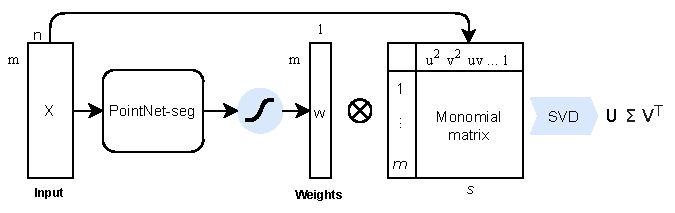
\includegraphics[width=1.0\textwidth]{consensus}
	\caption{}
	\label{fig:consensus}
\end{figure}

Because the fundamental matrix is a constraint expressed by 1 linear equation a basis of only 1  nullspace vector is needed from the singular value decomposition to construct it. But the method can also be used to learn constraints such as a homography or rigid 3D transformation that are constrained by 3 linear equations and therefore require a basis of 3 nullspace vectors. In that case the last 3 singular values from the SVD should be minimized in the loss function.

In the following sections the method used to extract the homography from the basis vectors will be explained. Two points that are related by a homography is expressed as follows. The monomials are grouped by parentheses.

\[
u \times Hv=0 \rightarrow
\]
\[
[u]_{\times} Hv=0 \rightarrow
\]
\[
\begin{pmatrix}
0 & -1 & u_y \\
1 & 0 & -u_x \\
-u_y & u_x & 0 \\
\end{pmatrix}
\begin{pmatrix}
h_{11} & h_{12} & h_{13} \\
h_{21} & h_{22} & h_{23} \\
h_{31} & h_{32} & h_{33} \\
\end{pmatrix}
\begin{pmatrix}
v_x \\
v_y \\
1 \\
\end{pmatrix}
=
\begin{pmatrix}
0 \\
0 \\
0 \\
\end{pmatrix}
\rightarrow
\]
\[
\begin{cases}
-h_{21} (v_x) \ \ \ \ - h_{22} (v_y) \ \ \ \ - h_{23} (1) \ \ \ + h_{31} (v_x u_y) + h_{32} (v_y u_y) + h_{33} (u_y) = 0 \\
\ \ h_{11} (v_x) \ \ \ \ \ + h_{12} (v_y) \ \ \ \ + h_{13} (1) \ \ -h_{31} (v_x u_x) -h_{32} (v_y u_x) - h_{33} (u_x) = 0 \\
-h_{11} (v_x u_y) -h_{12} (v_y u_y) -h_{13} (u_y) + h_{21} (v_x u_x) + h_{22} (v_y u_x) + h_{23} (u_x) = 0 \\
\end{cases}
\]

The monomials are the same as for the fundamental constraint, which means that the same Vandermonde matrix $M$ can be used. But because an homography is constrained by $r=3$ linear equations the last 3 singular values of the SVD should be minimized during training.

Extract 3 basis vectors from the nullspace which will be the 3 rightmost columns of $ V $ in the SVD of $diag(\textbf{w})M$.

\[
B = 
\begin{pmatrix}
\textbf{v}_7 & \textbf{v}_8 & \textbf{v}_9
\end{pmatrix}
\in \mathbb{R}^{9x3}
\]

The 3 linear equations of the homography are tangled which means that the elements of $B$ can not be directly mapped onto the elements in $H$. Notice that the first equation of $H$ does not contain $u_y$ and the second equation of $H$ does not contain $u_x$. We can exploit this fact to perform a change of basis from $B \in \mathbb{R}^{9x3}$ to $B' \in \mathbb{R}^{9x2}$ that should have the following structure.

\begin{center}
\begin{tabular}{ c c c }
	Monomial & Structure of $B'$ & Corresponding element in $H$ \\
	$u_x v_x$ & \multirow{9}{*}{
$\begin{pmatrix}
	0 & . \\
	0 & . \\
	0 & . \\
	. & 0 \\
	. & 0 \\
	. & 0 \\
	. & . \\
	. & . \\
	. & . \\
\end{pmatrix}$
} & \multirow{9}{*}{
$\begin{pmatrix}
 & h_{31} \\
 & h_{32} \\
 & h_{33} \\
h_{31} &   \\
h_{32} &   \\
h_{33} &   \\
h_{21} & h_{11} \\
h_{22} & h_{12} \\
h_{23} & h_{13} \\
\end{pmatrix}$
} \\
	$u_x v_y$ & \\
	$u_x \ \ \ \ $ & \\    
	\hline
	$u_y v_x$ & \\
	$u_y v_y$ & \\
	$u_y \ \ \ \ $ & \\    
	\hline
	$\ \ \ \ v_x$ & \\
	$\ \ \ \ v_y$ & \\
	$\ \ \ \ 1$ & \\
\end{tabular}
\end{center}

To perform the change of basis to get the structure of $B'$ we use the nullspace $\textbf{n}_1 \in \mathbb{R}^{3\times 1}$ of rows 1, 2 and 3 from $B$, and the nullspace $\textbf{n}_2 \in \mathbb{R}^{3x1}$ of row 4, 5, 6 from $B$.

\[
A_1 = 
\begin{pmatrix}
b_{11} & b_{12} & b_{13} \\
b_{21} & b_{22} & b_{23} \\
b_{31} & b_{32} & b_{33} \\
\end{pmatrix},
A_2 = 
\begin{pmatrix}
b_{41} & b_{42} & b_{43} \\
b_{51} & b_{52} & b_{53} \\
b_{61} & b_{62} & b_{63} \\
\end{pmatrix}
\]
\[
\textbf{n}_1 = \textit{"rightmost column of right-singular vectors of A1"}
\]
\[
\textbf{n}_2 = \textit{"rightmost column of right-singular vectors of A2"}
\]
\[
\textbf{b}^{n_1} = B\textbf{n}_1
\]
\[
\textbf{b}^{n_2} = B\textbf{n}_2
\]

Now the $\textbf{b}^{n_1}$ and $\textbf{b}^{n_2}$ basis vectors will have the following structure as desired.

\[
\textbf{b}^{n_1} =
\begin{pmatrix}
0 \\
0 \\
0 \\
. \\
. \\
. \\
. \\
. \\
. \\
\end{pmatrix},
\textbf{b}^{n_2} =
\begin{pmatrix}
. \\
. \\
. \\
0 \\
0 \\
0 \\
. \\
. \\
. \\
\end{pmatrix},
\]

The basis vectors have zeros at the correct place. The next step is to adjust the scale so that row 4, 5 and 6 of $\textbf{b}^{n_1}$ and row 1, 2 and 3 of $\textbf{b}^{n_2}$ have the same norm because they both represent the same elements $h_{31}$, $h_{32}$ and $h_{33}$. We also make sure they have the same sign.

\[
s = \sign(b^{n_2}_1 + b^{n_2}_2 + b^{n_2}_3) \sign(b^{n_1}_4 + b^{n_1}_5 + b^{n_1}_6)
\]

$s$ will be -1 if they have different signs, or 1 if they are the same sign.

\[
B'=
\begin{pmatrix}
\textbf{b}^{n_1} / \norm{(b^{n_1}_4 \ b^{n_1}_5 \ b^{n_1}_6)
} &
\textbf{b}^{n_2} / \norm{(b^{n_2}_1 \ b^{n_2}_2 \ b^{n_2}_3)} s
\end{pmatrix}
\in \mathbb{R}^{9x2}
\]

It is now possible to assign the elements of $H$ by pattern matching.

\[
H=
\begin{pmatrix}
\ \ b'_{72} & \ \ b'_{82} & \ \ b'_{92} \\
\ \ b'_{71} & \ \ b'_{81} & \ \ b'_{91} \\
-b'_{41} & -b'_{51} & -b'_{61} \\
\end{pmatrix}
\]

The method not only works for predicting the fundamental or homographic relationship between points, but can also be used for 3D rigid transformations.

\[
v=Ru+t \rightarrow
\]
\[
Ru+t-v=0 \rightarrow
\]
\[
\begin{pmatrix}
r_{11} & r_{12} & r_{13} \\
r_{21} & r_{22} & r_{23} \\
r_{31} & r_{32} & r_{33} \\
\end{pmatrix}
\begin{pmatrix}
u_x \\
u_y \\
y_z \\
\end{pmatrix}
+
\begin{pmatrix}
t_x \\
t_y \\
t_z \\
\end{pmatrix}
-
\begin{pmatrix}
v_x \\
v_y \\
v_z \\
\end{pmatrix}
=
\begin{pmatrix}
0 \\
0 \\
0 \\
\end{pmatrix}
\rightarrow
\]
\[
\begin{cases}
r_{11} (u_x) + r_{12} (u_y) + r_{13} (u_z) + t_x (1) - (v_y) = 0 \\
r_{21} (u_x) + r_{22} (u_y) + r_{23} (u_z) + t_y (1) - (v_x) = 0 \\
r_{31} (u_x) + r_{32} (u_y) + r_{33} (u_z) + t_z (1) - (v_z) = 0 \\
\end{cases}
\]

The monomials in the parentheses form the following Vandermonde matrix.

\[
M=
\begin{pmatrix}
u_{x,1} & u_{y,1} & u_{z,1} & v_{x,1} & v_{y,1} & v_{z,1} & 1 \\
 & & & \vdots & & & \\
u_{x,m} & u_{y,m} & u_{z,m} & v_{x,m} & v_{y,m} & v_{z,m} & 1 \\
\end{pmatrix}
\]

The constraint of $r=3$ linear equations is satisfied for all inliers if

\[
\diag(\textbf{w})
M
\begin{pmatrix}
r_{11} & r_{21} & r_{31} \\
r_{12} & r_{22} & r_{32} \\
r_{13} & r_{23} & r_{33} \\
-1 & 0 & 0 \\
0 & -1 & 0 \\
0 & 0 & -1 \\
t_x & t_y & t_z \\
\end{pmatrix}
=
\begin{pmatrix}
0 \\
\vdots \\
0 \\
\end{pmatrix}
^{mx1}
\]

Similar to before $R$ and $t$ is extracted from the null vectors of $\diag(\textbf{w})M$. The null vectors are the 3 rightmost singular vectors in the SVD. The 3 null vectors form a basis matrix $B$ on which a change of basis is performed to untangle the components $v_x$, $v_y$ and $v_z$ into a new structure $B'$ where $R$ and $t$ are easy to extract.

\begin{center}
	\begin{tabular}{ c c c }
		Monomial & Structure of $B'$ &  \\
		$u_x$ & \multirow{7}{*}{
			$\begin{pmatrix}
			r_{11} & r_{21} & r_{31} \\
			r_{12} & r_{22} & r_{32} \\
			r_{13} & r_{23} & r_{33} \\
			-1 & 0 & 0 \\
			0 & -1 & 0 \\
			0 & 0 & -1 \\
			t_x & t_y & t_z \\
			\end{pmatrix}$
		} \\
		$u_y$ & \\
		$u_z$ & \\    
		\hline
		$v_x$ & \\
		$v_y$ & \\
		$v_z$ & \\    
		\hline
		$1$ & \\
	\end{tabular}
\end{center}

\[
B'=
-
\begin{pmatrix}
b_{41} & b_{42} & b_{43} \\
b_{51} & b_{52} & b_{53} \\
b_{61} & b_{62} & b_{63} \\
\end{pmatrix}^{-1}
\begin{pmatrix}
b_{11} & b_{12} & b_{13} \\
b_{21} & b_{22} & b_{23} \\
b_{31} & b_{32} & b_{33} \\
b_{41} & b_{42} & b_{43} \\
b_{51} & b_{52} & b_{53} \\
b_{61} & b_{62} & b_{63} \\
b_{71} & b_{72} & b_{73} \\
\end{pmatrix}
=
\begin{pmatrix}
r_{11} & r_{21} & r_{31} \\
r_{12} & r_{22} & r_{32} \\
r_{13} & r_{23} & r_{33} \\
-1 & 0 & 0 \\
0 & -1 & 0 \\
0 & 0 & -1 \\
t_x & t_y & t_z \\
\end{pmatrix}
\]

However this holds for any affine transformation, to enforce the rotation manifold constraint an additional regularizer loss term is added.

\[
\mathcal{L}_r=\log(1 + || RR^T - I_{3\times3} ||)
\]

\subsection{Improving training convergence}

After some initial attempts at training the consensus maximization network for hagiographies on the output of the keypoint network, it was clear that it was next to impossible to get the training to converge on a good solution. Applying some additional techniques not described in the original paper resolved the issue.

Firstly the points should be transformed into a different basis before they are fed into the consensus maximization network. The change of basis ensures that the coordinates are scaled so that their maximum magnitude is 1, and the origin is centered in the middle of the image and not in the top left corner.

\[
G=
\begin{pmatrix}
W & 0 & W/2 \\
0 & W & H/2 \\
0 & 0 & 1 \\
\end{pmatrix}
\]
\[
p' = G^{-1} p
\]
Where $p$ is the output point from the keypoint network, $W$ and $H$ is the width and height of the image respectively, and $p'$ is the new altered point used as input. The homography $H$ predicted by the consensus maximization network will be in this new basis $G$ and needs to be altered in order to use it in our standard pixel coordinate basis as follows.

\[
H' = G H G^{-1}
\]

The second method to improve convergence during training is to normalize the rows of the Vandermonde matrix as follows.

\[
M_n' = \frac{M_n}{||M_n||}
\]

For all $n$ rows of the Vandermonde matrix $M$.







\iffalse

\subsection{CNN architectures}

In order to predict depth and motion from monocular images two different CNN architectures will be implemented.

\paragraph{SfMLearner} This is the architecture from \cite{sfmlearner}. The authors use a DispNet\cite{dispnet} architecture to predict depth maps at four different scales, and a ResNet18\cite{resnet} architecture with modified decoder to predict pose updates in an euler angle axis representation.

\paragraph{Monodepth2} This is the architecture from \cite{monodepth2}. The authors use a ResNet18 architecture instead of a DispNet architecture to predict depth estimates. They make this choice because its a smaller and faster architecture. Similarly they use a ResNet18 architecture with modified decoder to predict the pose updates in an euler angle axis representation.

\subsection{Differentiable depth image warping}
\label{sec:diffwarp}

Central to all previous methods in the related work section is the differentiable depth image warp operation in the loss function of the CNN networks. Given the intrinsic camera matrix:

\[
K = 
\begin{pmatrix}
f_x & s & x_0 \\
0 & f_y & y_0 \\
0 & 0   & 1
\end{pmatrix}
\]

And the predicted depth $ D_t(p_t) $ of pixel $ p_t $ of the target (current) frame. And the transform $ T_{t \rightarrow s} $ from the target to source (next/previous) frame:

\[
T_{t \rightarrow s} =
\begin{pmatrix}
\textbf{R} & \textbf{t} \\
0 & 1
\end{pmatrix}
\]

The position of the target pixel $ p_t $ in the source image $ p_s $ can be calculated in homogeneous coordinates as:

\[
p_s \sim K T_{t \rightarrow s} D_t(p_t) K^{-1} p_t 
\]

The pixel position $ p_s $ is however continuous and in order to sample the discrete source image $ I_s $ a differentiable bilinear sampling method is used. The method is described in \textit{spatial transformer networks}\cite{spatialtransformernetworks} and works by interpolating the neighbouring 4 pixels values (top-left, bottom-right) by the distance to the the continuous sampling point $ p_t $.

\subsection{Loss functions}
\label{sec:loss}

\paragraph{Photometric loss} Is defined as $ \mathcal{L}_p(I_t, \hat{I}_s)=|I_t - \hat{I}_s| $.

\paragraph{SSIM loss} Is defined as $ \mathcal{L}_{ssim}(I_t, \hat{I}_s)=\dfrac{1-\textrm{SSIM}(I_t, \hat{I}_s)}{2} $.

\paragraph{Combined loss} The photometric and SSIM loss is often combined and balanced using $ \mathcal{L}_{ps}(I_t, \hat{I}_s) = \alpha \mathcal{L}_{ssim} + (1-\alpha) \mathcal{L}_p $

\paragraph{Depth smooth loss} Is defined as $ \mathcal{L}_{smooth}(D_t)=|\delta_x^2 D_t|+|\delta_y^2 D_t| $. Not ideal because it can cause very fussy edges as seen in SfMLearner.

\paragraph{Edge aware depth smooth loss} Is defined as $ \mathcal{L}_{edge}(D_t)=|\delta_x D_t|e^{-|\delta_x I_t|} + |\delta_y D_t|e^{-|\delta_y I_t|} $. Applied in Monodepth2 giving sharper edges because the smoothness term is weighted to mostly affect areas with small photometric derivitive.

\paragraph{Velocity supervision loss} When a velocity measurement exists in the dataset a term to enforce scale accurate estimates can be added like $ \mathcal{L}_{v} = \bigr{|} \| \textbf{t}_{t \rightarrow s} \| - |v|\Delta t \bigr{|} $, as proposed in packnet\cite{packnet}.

\subsection{Handling occlusions}
\label{sec:occlusion}

\paragraph{Disparity loss} To encourage background depths (low disparities) in shadows of the depth map where occlusion has occurred a penalty on the disparity can be added $ \mathcal{L}_{o} =|d_t|. $

\paragraph{Minimum loss across frames} In SfMLearner the photometric loss is calculated for the previous and next frames compared to the current in the sequence. The pixel wise average across the frames are then used. This causes problems if a pixel is for example occluded in the previous frame, but visible in the current and next frame. In this situation the average loss will be pretty high even though a correct depth and transformation has been predicted, because of the occluded pixel. Instead Monodepth2 suggests to pick the minimum per pixel error over the frames which creates a more telling loss. 

\subsection{Handling model limitations}
\label{sec:modellimit}

In order to optimize using the photometric reprojecton error as the loss function two assumptions must hold. Firstly the scene must be static, meaning all objects in the scene must be still except the moving camera. Movement by cars and humans in the scene that is not due to the camera movement will cause problems. Secondly there must be photometric consistency between frames for the photometric error to make sense. This means that non lambertian surfaces, change in lighting, and change in exposure between frames will cause problems.

\paragraph{Explainability mask} The authors of \cite{sfmlearner} tackle this problem by having a CNN predict what pixels are valid to use in the photometric loss function. It shares the encoder of the pose predicting network but branches of into a different encoder which estimates a mask of the valid/explainable pixels. The loss function for the mask is the cross entropy loss compared to a mask filled with ones. The photometric loss function is augmented to include the explainability mask removing pixels that cannot be explained by the predicted depth and transformation. This encourages the mask to be filled with ones, but allows some slack due to pixels that can not be explained by the photometric loss.

\paragraph{Stationary pixels mask} The authors of \cite{monodepth2} introduced a mask to remove stationary pixels from the set of previous, current and next frame. This is done by creating a mask where the photometric error is smaller before applying the projection than after. This works because stationary pixels that have not moved in relation to the camera will of course have a small photometric loss without reprojection. This will remove pixels from the car dashboard and also nearby vehicles that are traveling at the same speed.

\subsection{Multi-scale estimation}

In the depth decoder 4 different scales of the depth map is created. In SfMLearner downsamples the target image to the size of the depth map when calculating the loss. The authors of Monodepth2 noticed that this creates holes in the depth prediction on some surfaces because it creates ambiguities for the pixels removed during downsampling. Their approach is instead to resize the depth map to the target image size using interpolation, which turns out to work better.

\fi